% \documentclass[12pt,a4paper,twoside,openright]{report}
\documentclass[12pt,a4paper,oneside,openright]{report}

\let\openright=\cleardoublepage



%%% Choose a language %%%

\newif\ifEN
\ENtrue   % uncomment this for english
%\ENfalse   % uncomment this for czech

%%% Configuration of the title page %%%

\newif\ifMFF
\MFFtrue % comment this out for the version with a big UK university logo
\def\UKName{Charles University in Prague} %this is only used in UK-logo-version
\def\UKFaculty{Faculty of Mathematics and Physics}

% Thesis type names, as used in several places in the title
%\def\ThesisTypeTitle{\ifEN BACHELOR THESIS \else BAKALÁŘSKÁ PRÁCE \fi}
\def\ThesisTypeTitle{\ifEN MASTER THESIS \else DIPLOMOVÁ PRÁCE \fi}
%\def\ThesisTypeTitle{\ifEN RIGOROUS THESIS \else RIGORÓZNÍ PRÁCE \fi}
%\def\ThesisTypeTitle{\ifEN DOCTORAL THESIS \else DISERTAČNÍ PRÁCE \fi}
%\def\ThesisGenitive{\ifEN bachelor \else bakalářské \fi}
\def\ThesisGenitive{\ifEN master \else diplomové \fi}
%\def\ThesisGenitive{\ifEN rigorous \else rigorózní \fi}
%\def\ThesisGenitive{\ifEN doctoral \else disertační \fi}
%\def\ThesisAccusative{\ifEN bachelor \else bakalářskou \fi}
\def\ThesisAccusative{\ifEN master \else diplomovou \fi}
%\def\ThesisAccusative{\ifEN rigorous \else rigorózní \fi}
%\def\ThesisAccusative{\ifEN doctoral \else disertační \fi}



%%% Fill in your details %%%

% (Note: \xxx is a "ToDo label" which makes the unfilled visible. Remove it.)
\def\ThesisTitle{Integration of the Embree Raycasting Library into a CSG Renderer}
\def\ThesisAuthor{Bc. Sebastian Schimper}
\def\YearSubmitted{2021}

% department assigned to the thesis
\def\Department{Department of Software and Computer Science Education}
% Is it a department (katedra), or an institute (ústav)?
\def\DeptType{Department}

\def\Supervisor{doc. Alexander Wilkie, Dr.}
\def\SupervisorsDepartment{Department of Software and Computer
	Science Education}

% Study programme and specialization
\def\StudyProgramme{Computer Science}
\def\StudyBranch{Computer Graphics and Game Development}

\def\Dedication{%
I owe a significant depth of gratitude to my supervisor, Prof. Alexander Wilkie, for the possibility to contribute to the development of a groundbreaking rendering system and for his help, support, and trust in me. I would also like to express sincere thankfulness towards Alban Fichet. His help and feedback were of crucial importance to my work. Additionally, I would like to thank various members of the Computer Graphics Group in Prague for numerous reviews and discussions, and the "Computer Graphics Stack Exchange" users Peter and Simon F, two strangers on the internet, for offering help when no help was available, thus preventing me from going completely nuts. I am grateful to my brother for helping me resolving various issues concerning Latex. Another person I wish to thank is Solange Petracchi, my contact person at Charles University, for getting me out of trouble multiple times during my years of study and for her moral support.
Finally, I would like to thank my family, friends, and Monika for their love and support during difficult times.
}

\def\AbstractEN{%
Modern High-Performance Ray Casting toolkits, such as the Intel Embree library, a de facto industry standard, are a cornerstone of the high-performance levels seen in current CPU rendering. The purpose of Embree is its integration into professional image synthesis environments to accelerate rendering scenes with complex geometry, usually being composed of a large number of primitives. Unfortunately, Embree does not offer support for rendering constructive solid geometry (CSG), solids composed of a manageable amount of primitive solids by using set operations. This is a significant drawback since CSG are an intuitive and powerful option for describing complex geometry.
In this thesis, we describe the integration of Embree into the predictive rendering system ART and propose a method for rendering CSG by combining the traversal of Embree's and Art's internal ray acceleration data structures. The tests we conducted with virtual scenes containing CSG showed that our method is competitive with the original ART renderer and often even faster.
% ABSTRACT IS NOT A COPY OF YOUR THESIS ASSIGNMENT!
}

\def\AbstractCS{%
\xxx{You will need to submit both Czech and English abstract to the SIS, no matter what language you use in the thesis. If writing in English, translate the contents of \texttt{\textbackslash{}AbstractEN} into this field. In case you do not speak czech, your supervisor should be able to help you with the translation.}
}

% 3 to 5 keywords (recommended), each enclosed in curly braces.
% Keywords are useful for indexing and searching for the theses by topic.
\def\Keywords{{Raycasting,} {CSG}, {Embree}}


% If your abstracts are long and do not fit in the infopage, you can make the
% fonts a bit smaller by this setting. (Also, you should try to compress your abstract more.)
% Alternatively, consider increasing the size of the page by uncommenting the
% geometry modification in thesis.tex.
\def\InfoPageFont{}
%\def\InfoPageFont{\small}  %uncomment to decrease font size

\ifEN\relax\else
% If you are writing a czech thesis, you additionally need to fill in the
% english translation of the metadata here!
\def\ThesisTitleEN{\xxx{Thesis title in English}}
\def\DepartmentEN{\xxx{Name of the department in English}}
\def\DeptTypeEN{\xxx{Department}}
\def\SupervisorsDepartmentEN{\xxx{Superdepartment}}
\def\StudyProgrammeEN{\xxx{study programme}}
\def\StudyBranchEN{\xxx{study branch}}
\def\KeywordsEN{%
\xxx{{key} {words}}
}
\fi


\usepackage[a-2u]{pdfx}

\ifEN\else\usepackage[czech,shorthands=off]{babel}\fi
\usepackage[utf8]{inputenc}
\usepackage[T1]{fontenc}

% See https://en.wikipedia.org/wiki/Canons_of_page_construction before
% modifying the size of printable area. LaTeX defaults are great.
% If you feel it would help anything, you can enlarge the printable area a bit:
%\usepackage[textwidth=390pt,textheight=630pt]{geometry}
% The official recommendation expands the area quite a bit (looks pretty harsh):
%\usepackage[textwidth=145mm,textheight=247mm]{geometry}

%%% FONTS %%%
\usepackage{lmodern} % TeX "original" (this sets up the latin mono)

% Optionally choose an override for the main font for typesetting
\usepackage[mono=false]{libertinus} % popular for comp-sci (ACM uses this)
%\usepackage{tgschola} % Schoolbook-like (gives a bit of historic feel)
%\usepackage[scale=0.96]{tgpagella} % Palladio-like (popular in formal logic).

% Optionally choose a custom sans-serif fonts (e.g. for figures and tables).
% Default sans-serif font is usually Latin Modern Sans. Some font packages
% (e.g. libertinus) replace that with a better matching sans-serif font.
%\usepackage{tgheros} % recommended and very readable (Helvetica-like)
%\usepackage{FiraSans} % looks great
% DO NOT typeset the main text in sans-serif font!
% The serifs make the text easily readable on the paper.

% IMPORTANT FONT NOTE: Some fonts require additional PDF/A conversion using
% the pdfa.sh script. These currently include only 'tgpagella'; but various
% other fonts from the texlive distribution need that too (mainly the Droid
% font family).


% some useful packages
\usepackage{amsmath,amsfonts,amsthm,bm}
\usepackage{graphicx}
\usepackage{subfig}
\usepackage{xcolor}
\usepackage{booktabs}
\usepackage{caption}
\usepackage{floatrow}

% listings
\usepackage{enumitem}

% load bibliography tools
% \usepackage[backend=bibtex,natbib,style=numeric,sorting=none]{biblatex}

% alternative with alphanumeric citations (more informative than numbers):
%\usepackage[backend=bibtex,natbib, style=ACM-Reference-Format, citestyle=authoryear]{biblatex}

%\usepackage[backend=bibtex,natbib, style=ACM-Reference-Format, citestyle=authoryear]{biblatex}


\usepackage[backend=bibtex,natbib, style=ACM-Reference-Format, citestyle=authoryear-icomp, maxcitenames=1]{biblatex}

\let\oldcite\cite
\renewcommand*\cite[1]{[\oldcite{#1}]}

%
% alternatives that conform to iso690
% (iso690 is not formally required on MFF, but may help elsewhere):
%\usepackage[backend=bibtex,natbib,style=iso-numeric,sorting=none]{biblatex}
 %\usepackage[backend=bibtex,natbib,style=iso-alphabetic]{biblatex}
%
% additional option choices:
%  - add `giveninits=true` to typeset "E. A. Poe" instead of full Edgar Allan
%  - `terseinits=true` additionaly shortens it to nature-like "Poe EA"
%  - add `maxnames=10` to limit (or loosen) the maximum number of authors in
%    bibliography entry before shortening to `et al.` (useful when referring to
%    book collections that may have hundreds of authors)
%  - for additional flexibility (e.g. multiple reference sections, etc.),
%    remove `backend=bibtex` and compile with `biber` instead of `bibtex` (see
%    Makefile)
%  - `sorting=none` causes the bibliography list to be ordered by the order of
%    citation as they appear in the text, which is usually the desired behavior
%    with numeric citations. Additionally you can use a style like
%    `numeric-comp` that compresses the long lists of citations such as
%    [1,2,3,4,5,6,7,8] to simpler [1--8]. This is especially useful if you plan
%    to add tremendous amounts of citations, as usual in life sciences and
%    bioinformatics.
%  - if you don't like the "In:" appearing in the bibliography, use the
%    extended style (`ext-numeric` or `ext-alphabetic`), and add option
%    `articlein=false`.
%
% possibly reverse the names of the authors with the default styles:
%\DeclareNameAlias{default}{family-given}

% load the file with bibliography entries
\addbibresource{bibliography/thesis_bibliography}


% remove this if you won't use fancy verbatim environments
\usepackage{fancyvrb}

% remove this if you won't typeset TikZ graphics
\usepackage{tikz}
\usetikzlibrary{positioning} %add libraries as needed (shapes, decorations, ...)

% remove this if you won't typeset any pseudocode
\usepackage{algpseudocode}
\usepackage{algorithm}

% remove this if you won't list any source code
\usepackage{listings}

% for clickable links in appendix
\usepackage{hyperref}

\hypersetup{unicode}
\hypersetup{breaklinks=true}

\usepackage[noabbrev]{cleveref}


% various forms of TODOs (you should remove this before submitting)
\usepackage[textsize=tiny, backgroundcolor=yellow!25, linecolor=black!25]{todonotes}
\newcommand{\xxx}[1]{\textcolor{red!}{#1}}

 % remove this before compiling the final version


% use this for typesetting a chapter without a number, e.g. intro and outro
\def\chapwithtoc#1{
\chapter*{#1}
\addcontentsline{toc}{chapter}{#1}
}

% If there is a line/figure overflowing into page margin, this will make the
% problem evident by drawing a thick black line at the overflowing spot. You
% should not disable this.
\overfullrule=3mm

% The maximum stretching of a space. Increasing this makes the text a bit more
% sloppy, but may prevent the overflows by moving words to next line.
\emergencystretch=1em

\ifEN
\theoremstyle{plain}
\newtheorem{thm}{Theorem}
\newtheorem{lemma}[thm]{Lemma}
\newtheorem{claim}[thm]{Claim}
\newtheorem{defn}{Definition}
\theoremstyle{remark}
\newtheorem*{cor}{Corollary}
\else
\theoremstyle{plain}
\newtheorem{thm}{Věta}
\newtheorem{lemma}{Lemma}
\newtheorem{claim}{Tvrzení}
\newtheorem{defn}{Definice}
\theoremstyle{remark}
\newtheorem*{cor}{Důsledek}
\fi

\newenvironment{myproof}{
  \par\medskip\noindent
  \textit{\ifEN Proof \else Důkaz \fi}.
}{
\newline
\rightline{$\qedsymbol$}
}

% real/natural numbers
\newcommand{\R}{\mathbb{R}}
\newcommand{\N}{\mathbb{N}}

% asymptotic complexity
\newcommand{\asy}[1]{\mathcal{O}(#1)}

% listings and default lstlisting config (remove if unused)
\DeclareNewFloatType{listing}{}
\floatsetup[listing]{style=ruled}

\DeclareCaptionStyle{thesis}{style=base,font={small,sf},labelfont=bf,labelsep=quad}
\captionsetup{style=thesis}
\captionsetup[algorithm]{style=thesis,singlelinecheck=off}
\captionsetup[listing]{style=thesis,singlelinecheck=off}

\ifEN\floatname{listing}{Listing}
\else\floatname{listing}{Výpis kódu}\fi
\lstset{%
  language=C++,
  tabsize=2,
  showstringspaces=false,
  basicstyle=\footnotesize\tt\color{black!75},
  identifierstyle=\bfseries\color{black},
  commentstyle=\color{green!50!black},
  stringstyle=\color{red!50!black},
  keywordstyle=\color{blue!75!black}}

% Czech versions of the used cleveref references (It's not as convenient as in
% English because of declension, cleveref is limited to sg/pl nominative. Use
% plain \ref to dodge that.)
\ifEN\relax\else
\crefname{chapter}{kapitola}{kapitoly}
\Crefname{chapter}{Kapitola}{Kapitoly}
\crefname{section}{sekce}{sekce}
\Crefname{section}{Sekce}{Sekce}
\crefname{subsection}{sekce}{sekce}
\Crefname{subsection}{Sekce}{Sekce}
\crefname{subsubsection}{sekce}{sekce}
\Crefname{subsubsection}{Sekce}{Sekce}
\crefname{figure}{obrázek}{obrázky}
\Crefname{figure}{Obrázek}{Obrázky}
\crefname{table}{tabulka}{tabulky}
\Crefname{table}{Tabulka}{Tabulky}
\crefname{listing}{výpis}{výpisy}
\Crefname{listing}{Výpis}{Výpisy}
\floatname{algorithm}{Algoritmus}
\crefname{algorithm}{algoritmus}{algoritmy}
\Crefname{algorithm}{Algoritmus}{Algoritmy}
\newcommand{\crefpairconjunction}{ a~}
\newcommand{\crefrangeconjunction}{ a~}
\fi
 % use this file for various custom definitions


\begin{document}

% the layout is mandatory, edit only in dire circumstances

\pagestyle{empty}
\hypersetup{pageanchor=false}
\begin{center}

\ifMFF
\ifEN
\centerline{\mbox{
\includegraphics[width=166mm]{img/logo-en.pdf}}}
\else
\centerline{\mbox{
\includegraphics[width=166mm]{img/logo-cs.pdf}}}
\fi
\vspace{-8mm}
\else
{\large\noindent\UKName\par\medskip\par\UKFaculty }
\fi
\vfill

{\bf\Large\ThesisTypeTitle}

\vfill

\ifMFF\relax\else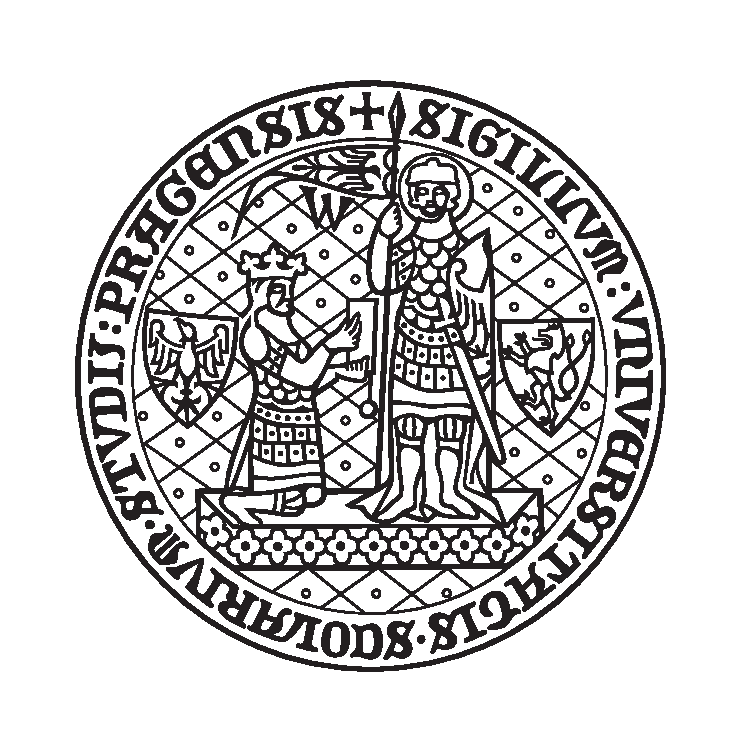
\includegraphics[width=70mm]{img/uklogo.pdf}

\vfill\fi

{\LARGE\ThesisAuthor}

\vspace{15mm}

{\LARGE\bfseries\ThesisTitle}

\vfill

\Department

\vfill

{
\centerline{\vbox{\halign{\hbox to 0.45\hsize{\hfil #}&\hskip 0.5em\parbox[t]{0.45\hsize}{\raggedright #}\cr
\ifEN Supervisor of the \ThesisGenitive thesis:
\else Vedoucí \ThesisGenitive práce: \fi
& \Supervisor \cr
\noalign{\vspace{2mm}}
\ifEN Study programme: \else Studijní program: \fi
& \StudyProgramme \cr
\noalign{\vspace{2mm}}
\ifEN Study branch: \else Studijní obor: \fi
& \StudyBranch \cr
}}}}

\vfill

\ifEN Prague \else Praha \fi
\YearSubmitted

\end{center}

\newpage

% remember to sign this!
\openright
\hypersetup{pageanchor=true}
\pagestyle{plain}
\pagenumbering{roman}
\vglue 0pt plus 1fill

\ifEN
\noindent
I declare that I carried out this \ThesisAccusative thesis independently, and only with the cited
sources, literature and other professional sources. It has not been used to obtain another
or the same degree.
\else
\noindent
Prohlašuji, že jsem tuto \ThesisAccusative práci vypracoval(a) samostatně a výhradně
s~použitím citovaných pramenů, literatury a dalších odborných zdrojů.
Tato práce nebyla využita k získání jiného nebo stejného titulu.
\fi

\ifEN
\medskip\noindent
I understand that my work relates to the rights and obligations under the Act No.~121/2000 Sb.,
the Copyright Act, as amended, in particular the fact that the Charles
University has the right to conclude a license agreement on the use of this
work as a school work pursuant to Section 60 subsection 1 of the Copyright~Act.
\else
\medskip\noindent
Beru na~vědomí, že se na moji práci vztahují práva a povinnosti vyplývající
ze zákona č. 121/2000 Sb., autorského zákona v~platném znění, zejména skutečnost,
že Univerzita Karlova má právo na~uzavření licenční smlouvy o~užití této
práce jako školního díla podle §60 odst. 1 autorského zákona.
\fi

\vspace{10mm}


\ifEN
\hbox{\hbox to 0.5\hsize{%
In \hbox to 6em{\dotfill} date \hbox to 6em{\dotfill}
\hss}\hbox to 0.5\hsize{\dotfill\quad}}
\smallskip
\hbox{\hbox to 0.5\hsize{}\hbox to 0.5\hsize{\hfil Author's signature\hfil}}
\else
\hbox{\hbox to 0.5\hsize{%
V \hbox to 6em{\dotfill} dne \hbox to 6em{\dotfill}
\hss}\hbox to 0.5\hsize{\dotfill\quad}}
\smallskip
\hbox{\hbox to 0.5\hsize{}\hbox to 0.5\hsize{\hfil Podpis autora\hfil}}
\fi

\vspace{20mm}
\newpage

% dedication

\openright

\noindent
\Dedication

\newpage

% mandatory information page

\openright

\vbox to 0.49\vsize{\InfoPageFont
\setlength\parindent{0mm}
\setlength\parskip{5mm}

\ifEN Title: \else Název práce: \fi
\ThesisTitle

\ifEN Author: \else Autor: \fi
\ThesisAuthor

\DeptType:
\Department

\ifEN Supervisor: \else Vedoucí bakalářské práce: \fi
\Supervisor, \SupervisorsDepartment

\ifEN Abstract: \AbstractEN \else Abstrakt: \AbstractCS \fi

\ifEN Keywords: \else Klíčová slova: \fi
\Keywords

\vss}\ifEN\relax\else\nobreak\vbox to 0.49\vsize{\InfoPageFont
\setlength\parindent{0mm}
\setlength\parskip{5mm}

Title:
\ThesisTitleEN

Author:
\ThesisAuthor

\DeptTypeEN:
\DepartmentEN

Supervisor:
\Supervisor, \SupervisorsDepartmentEN

Abstract:
\AbstractEN

Keywords:
\KeywordsEN

\vss}
\fi

\newpage

\openright
\pagestyle{plain}
\pagenumbering{arabic}
\setcounter{page}{1}


\tableofcontents

\chapwithtoc{Introduction}
\label{chap:intro}

Ray tracing is a powerful image synthesis technique used in 3D computer graphics, capable of simulating optical effects, such as reflection, refraction, and scattering, with a high degree of visual realism. For this reason, it offers a variety of applications: It is used in the entertainment industry, for product design, visual prototyping, and for creating visualizations in scientific research \cite [91-128]{peddie2019ray}. Reasons for the popularity of ray tracing algorithms are the physical plausibility of its generated images as well as their simplicity and "elegance". 

The origins of ray tracing can be traced back as far as 1968. At that time, a method was invented to shade wire-framed solids by shooting random light rays from virtual light sources to the scene geometry and, if an intersection would be found, placing a symbol at the intersection point \cite{appel1968some}. If enough rays were generated, there would be a high concentration of these symbols at regions with high light intensity, which would approximate physical realism. A decade later, an elaboration of this idea to a shading model that takes global information into account for calculating light intensities  \cite{whitted1979improved}, would revolutionize the computer graphics field.

\begin{figure} \label{fig:whitted_result}
	\centering
	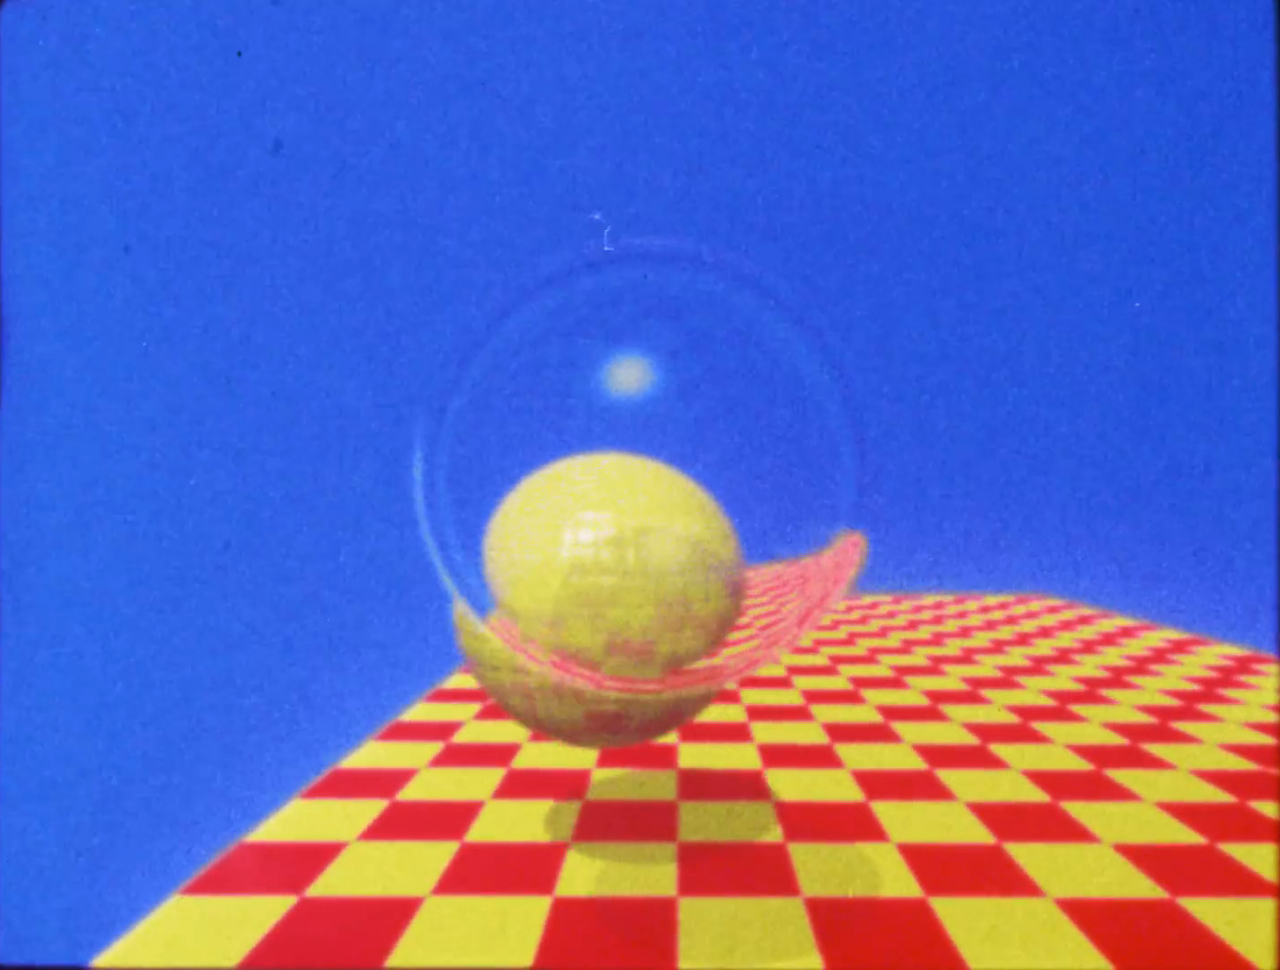
\includegraphics[width=.7\linewidth]{img/0 introduction/whitted_}
	\caption{A frame of an animation \cite{raytracingvideo} form \cite {whitted1979improved}, demonstrating recursive ray tracing, featuring a glass sphere circulating a second defuse sphere. Both are casting shadows on a diffuse checkerboard-like ground.}
	\label{fig:g}
\end{figure}

The calculation of intersection points between cast rays and scene geometry is a crucial part of ray tracing. How these points are calculated depends on the representation of geometric primitives in the scene. Primitives can be represented analytically or approximated by polygon meshes. Another possibility is the representation of a shape as a \emph{Constructive Solid Geometry (CSG)}. CSG is a hierarchical ordering of a set of primitive shapes to which Boolean set operations have been applied to. This form of representation enjoys popularity in e.g. Computer-aided geometric design.

Over the years, novel ray tracing algorithms were developed to increase the physical correctness of rendered images. However, ray tracing remains to this day a computationally demanding task. Much research was (and still is) devoted to accelerating the ray tracing procedure to compensate for its computational expense. Therefore, a wide range of researches focus on accelerating ray tracing algorithms to get better performances. Additionally, ray tracing is by nature is "embarrassingly parallel", meaning it is well suited for parallel processing by automatic vectorization. As Moore’s law predicted, the computational power in CPUs gradually increased. Nowadays, modern computers admit an integrated circuit with multiple cores on which the workload of ray tracing algorithms can be distributed. While ray tracing was considered impractical when it was pioneered, it has now become more accessible thanks to the increase of CPU power and specialized hardware.

Despite this, exploiting the computational power of modern processors to their full potential for ray tracing remains challenging. This particular reason served as the motivation for developing the award-winning (\cite{embreeAward}), open-source framework \emph{Embree} \cite{wald2014embree}. Embree offers a set of ray tracing kernels that maximize the compute capabilities of modern x86 CPU architectures.

One of the design goals behind Embree is to provide an easy integration of the framework into existing professional ray tracing environments to achieve high performance when ray tracing virtual scenes with high geometrical complexity.


\section*{Thesis subject and motivation}
The goal of this thesis is a successful integration of the Embree framework into the predictive rendering framework \emph{The Advanced Rendering Toolkit}, to facilitate the acceleration of ray tracing for constructive solid geometry.
The Advanced Rendering Toolkit will be referred to with its abbreviation \emph{ART} throughout this thesis. 

ART offers innovative features, such as efficient spectral rendering (by implementing the "Hero Wavelength Spectral Sampling" technique \cite{wilkie2014hero}), proper handling of bi-spectral materials (e.g., fluorescent surfaces) \cite{mojzik2018handling} and a physically plausible sky dome lighting model \cite{wilkie2013predicting}. Until the release of Mitsuba 2 \cite{nimier2019mitsuba}, ART was, to our best knowledge, the only rendering system that would support rendering polarization effects, and remains the sole open source rendering system to support bi-spectral reflectances. These features make ART an interesting environment for computer graphics researchers interested in the field of Predictive Rendering.

To ensure this features, ART relies on its proprietary internal data structures that diverge to a significant degree from those present in other popular rendering systems (e.g., pbrt \cite{pharr2016physically} or Mitsuba 2). Therefore, Embree's integration into ART is a non-trivial task, although Embree was developed with the intention of it being "used in existing renderers with minimal programmer effort" \cite[1]{wald2014embree}. Furthermore, Embree unfortunately does not directly support rendering CSG.

If a successful integration of Embree into ART could be achieved, a complex image synthesis system with unique predictive rendering features would be adapted to the industry standard of ray tracing. 

\section*{Thesis outline}

This thesis is structured as follows:

\begin{itemize}
	\setlength\itemsep{0.05em}
	
	\item \textbf{Chapter \ref{chap:fundamentals}} will provide fundamental background information, including a brief introduction to the ray tracing technique, explanations of the most common ray acceleration structures, and a brief overview of the functionality of the Embree framework.
	
	\item In \textbf{Chapter \ref{chap:technical_overview}} provides a description of Embree can be used for ray tracing and a brief introduction to ART, in which Embree will be integrated into.
	
	\item \textbf{Chapter \ref{chap:integration}} is dedicated to the description of our approach on the integration of Embree into ART, as well as the implementation of the CSG operations with Embree.
	
	\item Results obtained by testing our implementation on various virtual scenes are presented and evaluated in \textbf{Chapter \ref{chap:results}}.
	
	\item Lastly, \textbf{Appendix \ref{sec:embree_app}} provides a user guide for compiling ART with Embree support.
	
\end{itemize}

\chapter{Fundamentals}
\label{chap:fundamentals}

Under the term \emph{ray tracing} we understand the utilization of algorithms that involve the casting of virtual light rays for generating images. The purpose of these light rays is to archive high visual realism by the simulation of natural behavior in real life. 

The reason we are able to perceive nearby objects or persons is due to the fact that light, which is being emitted from light sources, either natural or artificial, is interacting with these objects or persons. It is being reflected off their surfaces towards our vision sensory organs after possibly being reflected a multiple times before from other surfaces.

The purpose of ray tracing algorithms is to imitate this behavior, usually by tracing these light rays in reverse order from the sensory organs (or a virtual camera or an "eye point") back to the emitting light source.

\begin{figure}[h]
	\centering
	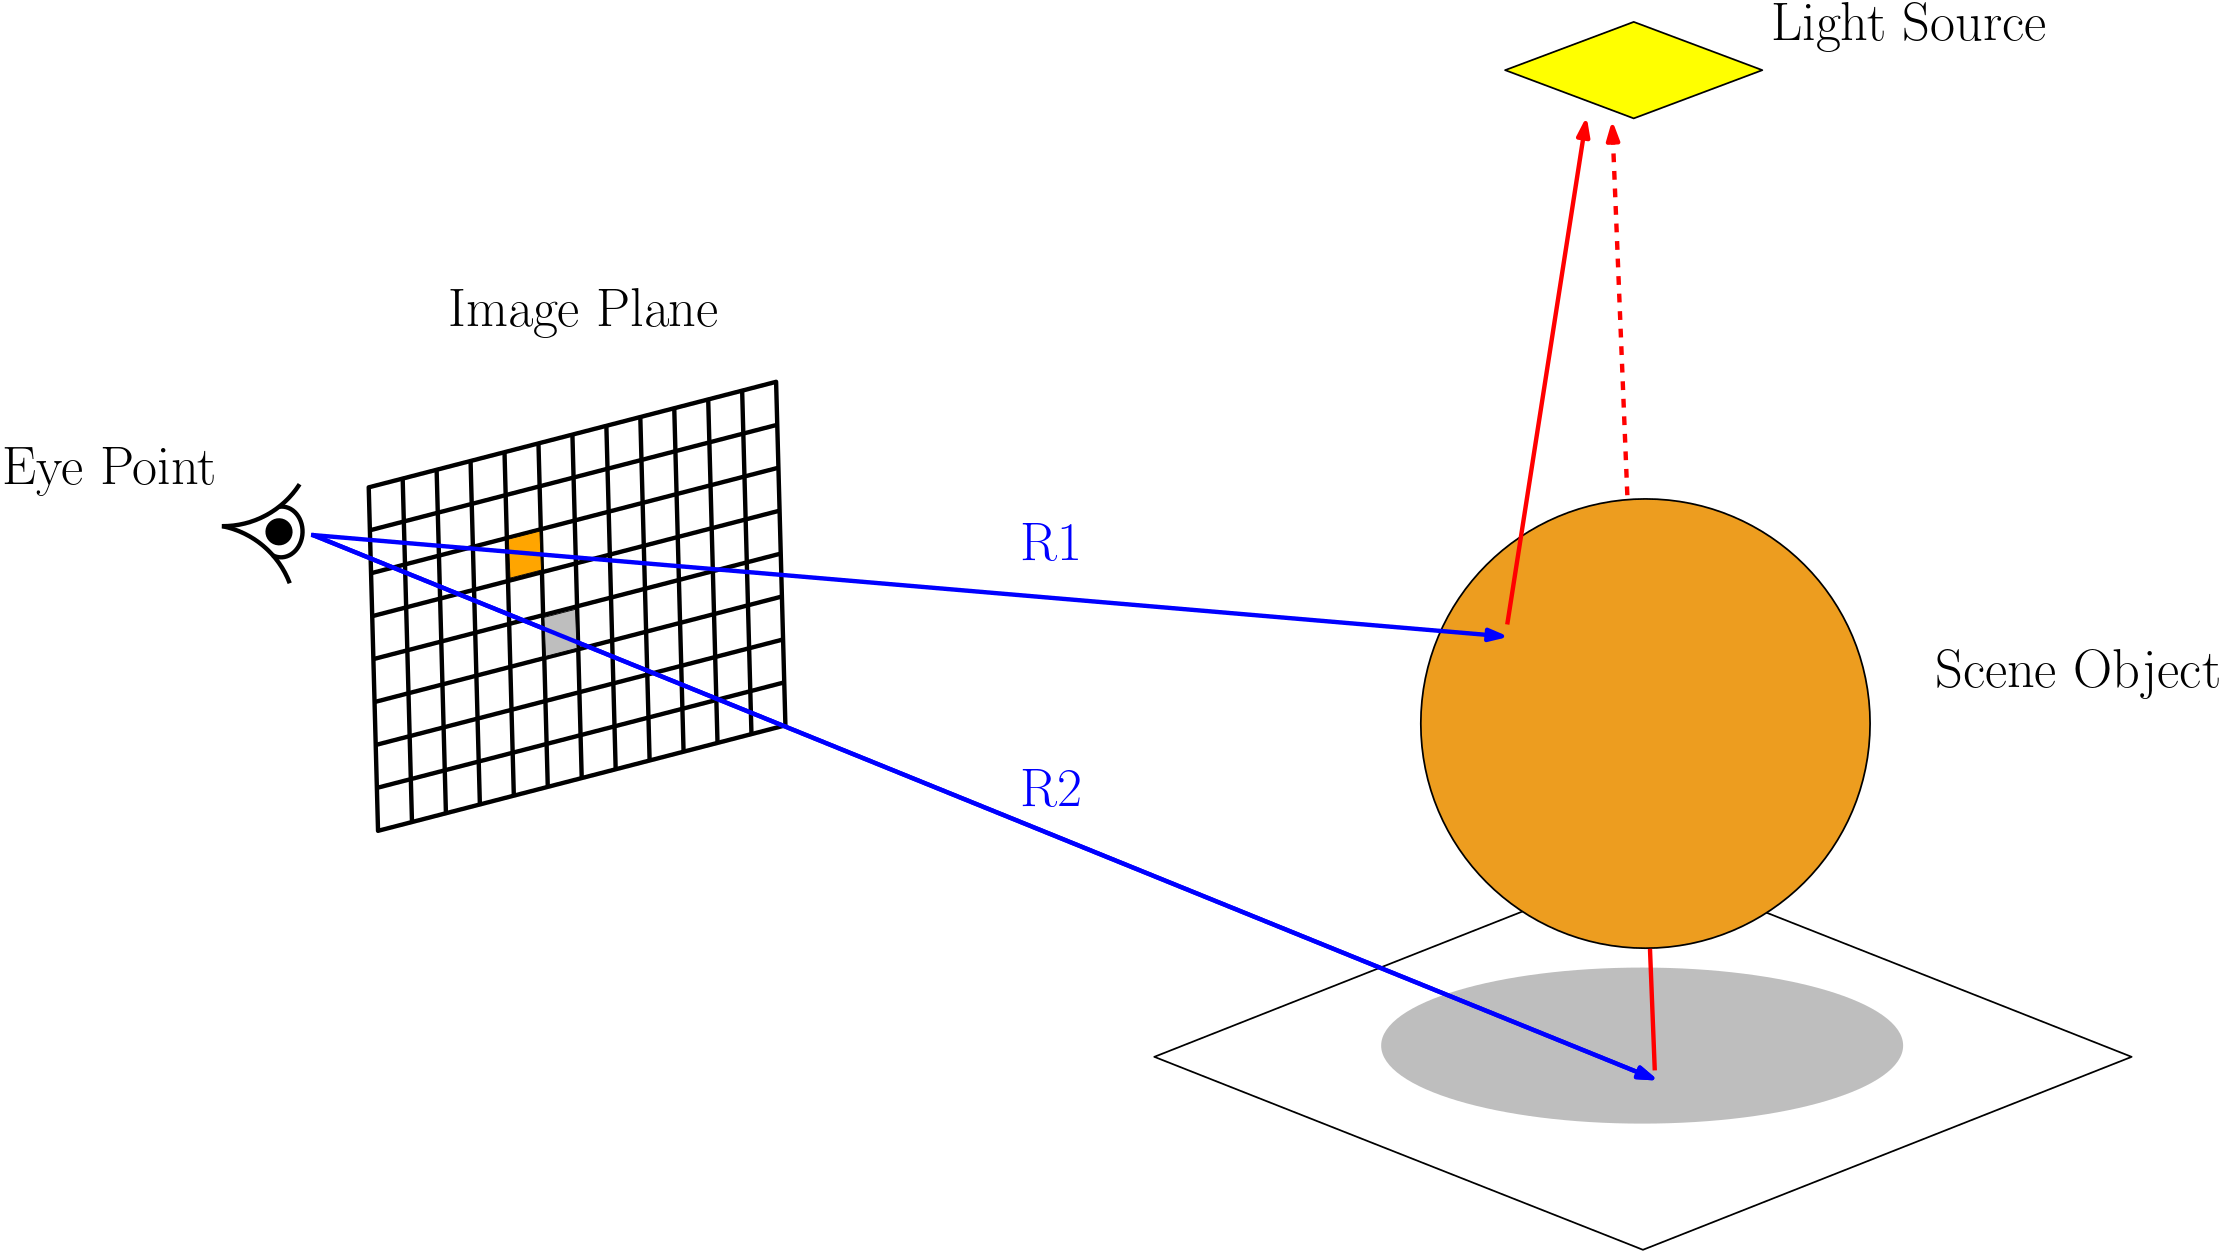
\includegraphics[width=.9\linewidth]{img/1 fundamentals/ray_tracing.png}
	\caption{Ray tracing procedure for calculating global illuminate.}
	\label{fig:raytracer_general}
\end{figure}

An advantage of these ray tracing algorithms is that the core procedure is straightforward when viewed from a theoretical point of view. Figure \ref{fig:raytracer_general} shows an example of a virtual scene. It is composed of an orange sphere, a white ground plane, and a light source. Furthermore, there exists an image plane on which the 2D image of the 3D scene will be projected. A ray is consisting of two components, an origin point and a direction vector. The "Eye Point" in \ref{fig:raytracer_general} will serve as the origin of the cast rays (sometimes, the Eye Point is referred to as camera or virtual camera). In the figure, the image plane is composed of multiple quadratic "cells" that represent the actual pixels of the resulting image. Through each of these cells, a ray is cast into the scene from the eye point. The subsequent step is to determine, whether that ray hit a particular geometry by performing intersection tests on all geometries in the scene \footnote{Testing all geometries present in a complex scene for intersection is a naive approach and not practical. Section \ref{sec:acceleration} introduces some common ray acceleration data structures to compensate for this.}. In case a geometry is hit, a secondary ray is generated with its origin at the intersection point and its direction toward the light source. In case this secondary light ray does not intersect any other geometry between its origin and the light source, this means that the first intersection point is exposed to light and the material color at that point is used for the corresponding pixel (see R1 in figure \ref{fig:raytracer_general}). Otherwise, the intersection point must be in shadow (see R2). This procedure generates an image with local illumination.

The following chapter is dedicated to providing background information on ray tracing, shape representation in rendering systems, and ray acceleration data structures. Furthermore, the Embree framework is introduced.

\section{Ray Tracing Algorithms}

The following section outlines the development of various ray tracing techniques. The pioneering work of \cite{appel1968some} and \cite{whitted1979improved} will be discussed, and the derivation to the rendering equation \cite{kajiya1986rendering}, whose solving via Monte Carlo integration is the aim of modern rendering environments, will be presented.

\subsection{Origins of Ray Tracing}
As briefly mentioned in the Introduction, ray tracing was pioneered in 1968 by \cite{appel1968some}. The aim of his work was to provide basic shading for wire framed solids, yielding a better communication of spatial relation and depth of objects in the rendered image.

In order to achieve this shading, virtual light rays are shot from a scene light source in random directions. Whenever one such ray intersects a geometry, a character or symbol (e.g. a small "plus"-symbol or square) is placed at that intersection point. If enough such rays would be cast, areas on the solid that are exposed to light would be shaded by these symbols.
The result would then come to be by inverting the shaded and non-shaded areas of the geometry.

The intensity of light $I$ incident to the light source is described by the following equation:

\begin{equation}
I = S\frac{\cos{\theta}}{{D}^2}
\end{equation}

\noindent where
\begin{itemize}
	\setlength\itemsep{0.05em}
	\item  $S$ is the intensity of the light source,
	\item  $\cos\theta$ is the angle between the ray and the surface normal at the intersection point, and
	\item  $D$ is the distance between intersection point and light source.
\end{itemize}

\begin{figure}[h]
	\centering
	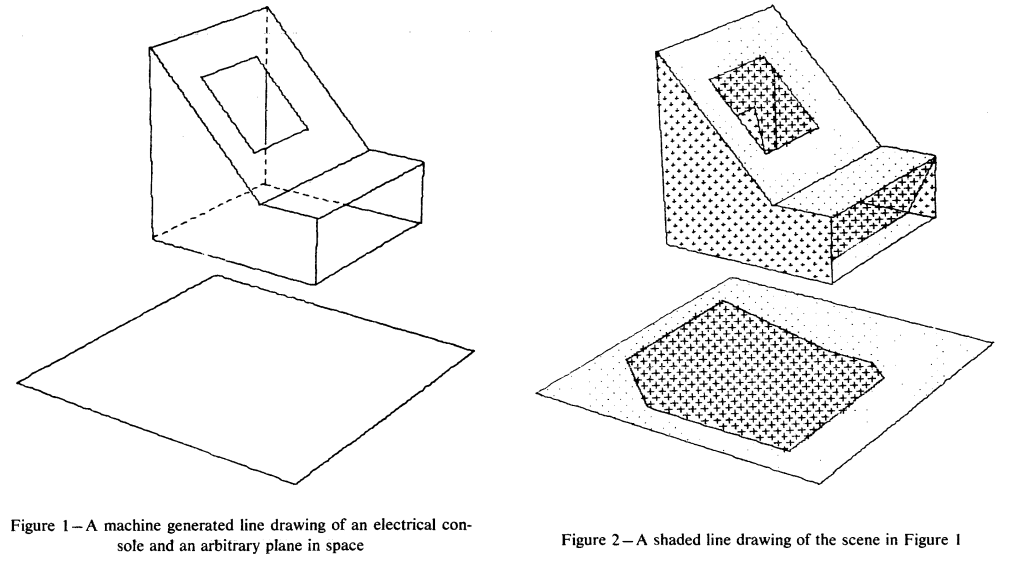
\includegraphics[width=1\linewidth]{img/1 fundamentals/appel_comp}
	\caption{Original figures from \cite{appel1968some}. The left figure shows plain solid geometry and the right figure shows the same solid with shading applied to it.}
	\label{fig:appel}
\end{figure}

Figure \ref{fig:appel} shows the result. Without the additional shading information, it would be difficult for the observer to perceive the position of the upper geometry relative to the plane.

In order to achieve convincing results, a high number of rays had to be generated ("Even for about 1000 light rays results were splotchy." \cite[p 3]{appel1968some}). At the time of publication, computational power of hardware could hardly be used for this approach.

The idea of casting rays later became a key utilization for a shading model that aimed for higher realism by taking the "global setting" of geometries into account \cite{whitted1979improved}. A variety of shading models existed at that time, which were able to convincingly display optical effects. However, these models usually worked only in special cases and not well with each other, as noted by Andrew Glassner in the preface of his book \citetitle{glassner1989introduction} \cite{glassner1989introduction}. Some models existed that were good at calculating reflection effects, but could not handle refraction effects well. And vice versa. 

\cite{whitted1979improved} introduced a shading model that would truthfully simulate reflection, shadows and refraction as well as the effects of other conventional shading models at that time.  

The model is partially derived from an empirical reflection model developed by \cite{phong1975illumination}, which assumes that light, which is reflected from a surface, is composed by three types of reflection: ambient reflection, diffuse reflection and specular reflection. The following equation describes this model:

\begin{equation} \label{eq:phong}
I = k_{a} + k_{d}\sum_{j}(n*L_{j}) + k_{s}\sum_{j}(n*L_{j}\prime)^{\alpha}
\end{equation}

\noindent where
\begin{itemize}
	\setlength\itemsep{0.05em}
	\item  $I$ is the reflected intensity,
	\item  $I_{a}$ is the ambient reflection coefficient,
	\item  $k_{d}$ is the diffuse reflection coefficient,
	\item  $k_{s}$ is the specular reflection coefficient,
	\item  $n$ is the unit surface normal at an intersection point,
	\item  $L_{j}$ is a vector in the direction of the $j$th light source,
	\item  $L_{j}\prime$ is a half vector between the eye point and the $j$th light source, and
	\item  $\alpha$ is the glossiness coefficient.
\end{itemize}

This model even nowadays finds popularity among real time graphics due to its low computational cost and convincing (although not physically plausible) results.
The model assumes furthermore that light sources are located at an infinite distance from the scene geometry, and thus, it does not account for objects within the scene acting as light sources. It was noted in \cite{newell1977progression}, that this assumption can critically affect the specular reflection component of Equation \ref{eq:phong}.

\begin{figure}[h]
	\centering
	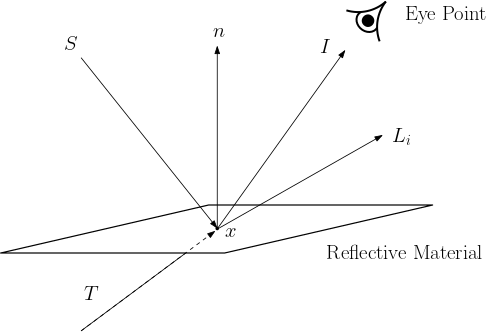
\includegraphics[width=.7\linewidth]{img/1 fundamentals/whitted.png}
	\caption{Light intensity propagated towards an observer being composed of a specular reflection component $S$ and a transmissive reflection component $T$.}
	\label{fig:whitted_model}
\end{figure}

As opposed to the Phong shading model, Whitted's model assumes that the light intensity $I$ arriving at the $Eye Point$ from the intersection point $x$ along the outgoing direction $\omega_{o}$ is conglomerated by a specular reflection component $S$, being propagated along direction $\omega_{s}$ and a transmission component $T$, being propagated along direction $\omega_{t}$. This is shown in Figure \ref{fig:whitted_model}.
The model is given by the equation:
\begin{equation} \label{eq:whitted}
I = k_{a} + k_{d}\sum_{j}(n*L_{j}) + k_{s}S + k_{t}T
\end{equation}

\noindent where
\begin{itemize}
	\setlength\itemsep{0.05em}
	\item  $S$ is the light intensity of the specular reflection
	\item  $T$ is the light intensity of the transmission, and
	\item  $k_{s}$ is the transmission coefficient
\end{itemize}
The ambient and diffuse term are maintained from Equation \ref{eq:phong}. 

The model is capable of generating images with a high degree of realism, preconditioned that the coefficients of equation \ref{eq:whitted} are reasonably chosen. Whitted noted in his paper that "for the best
accuracy they [the coefficients] should be functions that incorporate an
approximation of the Fresnel reflection". 
Generally, Equation \ref{eq:whitted} approximates the reflection of light towards an observer (or camera, or "Eye Point") from a single surface. However, in nature, light that is propagated towards a viewer from a surface most certainly has interacted with other surfaces before. If true realism of computer generated images is desired, these previous interactions have to be taken into consideration, even for virtual scenes with moderately complex geometry. An example of such an event can be seen in Figure \ref{fig:whitted_rays}.

\begin{figure}[h]
	\centering
	\subfloat[Light is being reflected from other surfaces before reaching the Eye Point.]{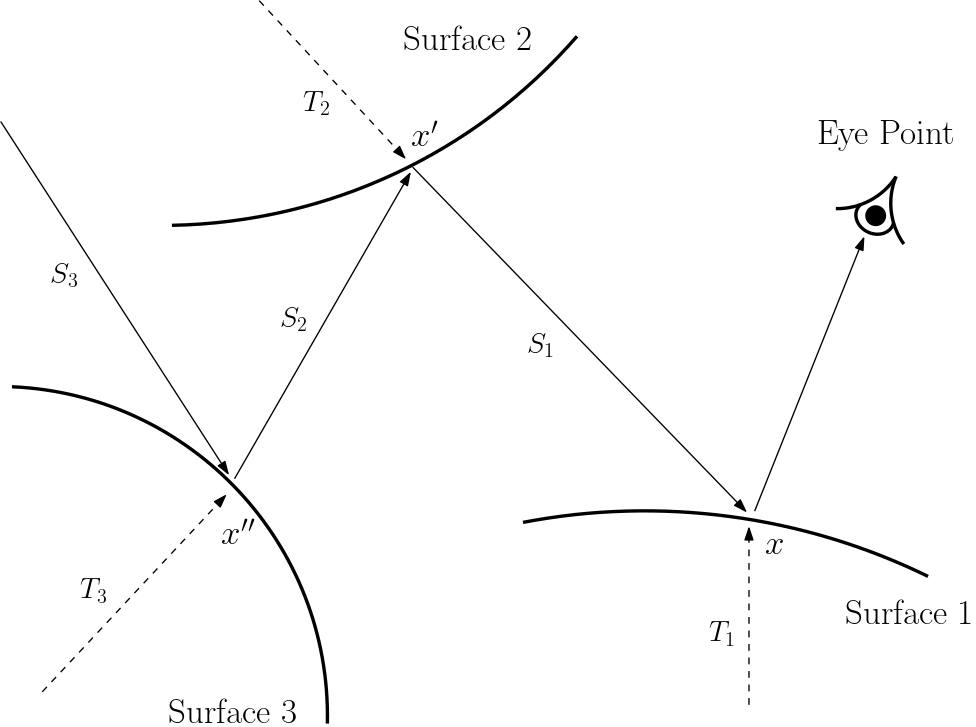
\includegraphics[width=.6\textwidth]{img/1 fundamentals/whitted_rays.png}\label{fig:whitted_rays}}
	\hfill
	\subfloat[Tree structure storing the individual reflection and transmission components.]{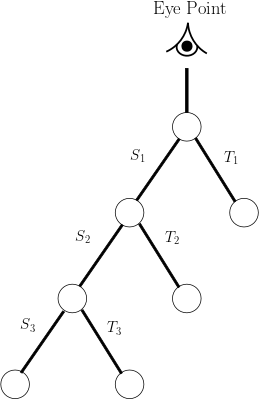
\includegraphics[width=.3\textwidth]{img/1 fundamentals/whitted_tree.png}\label{fig:whitted_tree}}
	\caption{Figures based on the original figures from the paper \citetitle{whitted1979improved} \cite{whitted1979improved}}
\end{figure}

This natural behavior is implemented in the following way. From the $Eye Point$, a ray is cast towards the virtual scene and a possible intersection point $x$ with the scene geometry is calculated. 
The transmission and specular component rays at that intersection point are then recursively calculated by Equation \ref{eq:whitted} and stored in a tree structure which is shown in Figure \ref{fig:whitted_tree}. 
Each node in this tree represents an intersection point and is furthermore associated with rays pointing towards each light source in the scene, which are correlated to the $L_{j}$ terms in Equation \ref{eq:whitted}. If one of these light rays $L_{j}$ intersect scene geometry before it reaches light source $j$, the intersection point corresponding to the tree node in question is not illuminated by that particular light source and consequentially the contribution of it to the reflection is not taken into consideration. To prevent a branch of the tree from growing infinitely large, it is truncated as soon as an attempt is made to access more storage than was previously made available for it. After such a tree is created, it is traversed recursively in order to calculate the light intensity at each node with Equation \ref{eq:whitted}, finally resulting in the calculation of the total light intensity that is reflected towards the $Eye Point$. Between two nodes, the intensity is attenuated according to a distance function between the intersection points, associated with the node and the node's parent node. 
Such trees are created and traversed for every pixel of the image plane. This procedure allows for the convincing display of a variety of optical effects with the help of a single model.

\subsection{The Rendering Equation}

In 1986, an integral equation was developed by Kajiya \cite{kajiya1986rendering}, that would describe the total reflected radiance towards an observer as the "sum" (or integral) of all light contributions over a hemisphere at a point on the surface. This mathematical model achieves high realism by taking direct illumination (light from light sources) and indirect illumination (light being reflected off other surfaces in the scene) into account.
The so-called \emph{rendering equation} is given by

\begin{equation}\label{eq:renderingeq}
L(x, \omega_{o}) = L_{e}(x, \omega_{o}) \int_{H(x)} L(x, \omega_{i})f_{r}(\omega_{i} \rightarrow \omega_{o})\cos\theta\partial\omega_{i}
\end{equation}

\noindent where
\begin{itemize}
	\setlength\itemsep{0.05em}
	\item  $L(x, \omega_{o})$ is the total reflected light intensity from a surface point $x$ towards the observer along the outgoing direction $\omega_{o}$,
	\item  $L_{e}(\omega_{o})$ is the radiance emitted at the surface point $x$ and propagated along $\omega_{o}$,
	\item  $H(x)$ is the hemisphere over surface point $x$,
	\item 	$L(x, \omega_{i})$ is the light intensity incident to $x$ along direction$\omega_{i}$, 
	\item  $f_{r}(\omega_{i} \rightarrow \omega_{o})$ is the bidirectional reflectance distribution function (BRDF), and 
	\item  $\cos\theta$ is a term, compensating for Lambert's cosine law.
\end{itemize}

For a better understanding of the individual terms of the rendering equation, a definition of radiance and a brief explanation of the \emph{bidirectional reflectance distribution function} and the local reflection equation is provided in the following subsections.
The information provided by these subsections are collated from the lecture notes of the course \citetitle{cg3} held at Charles University in Prague, Czech Republic \cite{cg3}, from the book \citetitle{pharr2016physically} \cite{pharr2016physically} and from the book \citetitle{hughesDamEtAl13} \cite{hughesDamEtAl13}.

\subsubsection{Definition of Radiance}

We define the \emph{radiance} of a source, sometimes informally referred to as "brightness", as the power per unit area $\partial A$ perpendicular to the ray in the direction $\omega_{o}$ and per unit solid angle that is propagated along it (see Figure \ref{fig:radiance}). This is described by the following equation:

\begin{equation}
L(\omega_{o}) = \frac{\partial^2\phi}{\partial\omega_{o}\partial A\cos\theta}
\end{equation}

\noindent where
\begin{itemize}
	\setlength\itemsep{0.05em}
	\item  $\omega_{o}$ is the outgoing direction
	\item  $\phi$ is flux or radiance per unit time
	\item  $A$ is the surface area, and
	\item  $\cos\theta$ a term for compensating Lambert's cosine law
\end{itemize}

\begin{figure}[h]
	\centering
	\subfloat[Radiance is defined as the radiant flux emitted, received or reflected per solid angle $\partial\omega_{o}$ per unit projected area $\partial A$.]{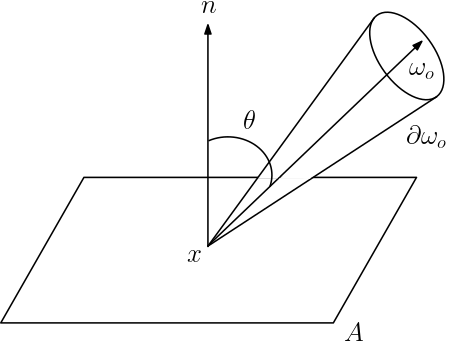
\includegraphics[width=.4\textwidth]{img/1 fundamentals/radiance.png}\label{fig:radiance}}
	\hfill
	\subfloat[The BRDF is a function defining how much light from the incoming direction$\omega_{i}$ is reflected towards the viewer along the outgoing direction $\omega_{o}$.]{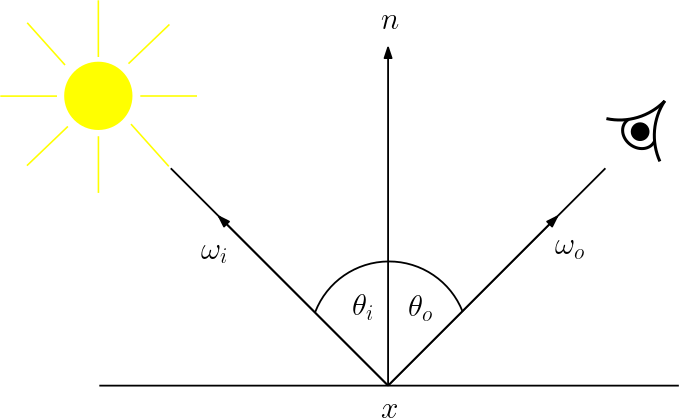
\includegraphics[width=.5\textwidth]{img/1 fundamentals/brdf.png}\label{fig:brdf}}
	\caption{Diagrams visualizing radiance (Figure \ref{fig:radiance}) and the BRDF (Figure \ref{fig:brdf}).}
\end{figure}

From this definition we can derive the bidirectional reflectance distribution function.

\subsubsection{Bidirectional Reflectance Distrubution Function (BRDF)}
The bidirectional reflectance distribution function (BRDF) is a mathematical model describing the reflection properties of a given surface. To be precise, it describes the probability of light energy, arriving at a point $x$ on a surface from direction $\omega_{i}$, being reflected along the reflection $\omega_{o}$. 
The BRDF model is defined by:

\begin{equation} \label{eq:brdf}
f_{r}(\omega_{i} \rightarrow \omega_{o}) = \frac{\partial L_{r}(\omega_{o})}{L_{i}(\omega_{i})\cos\theta\partial\omega_{i}}
\end{equation}

\noindent where
\begin{itemize}
	\setlength\itemsep{0.05em}
	\item  $L_{r}(\omega_{o})$ is the reflected light energy, and
	\item  $L_{i}(\omega_{i})$ is the incident light energy
\end{itemize}

Properties of BRDFs are the conservation of energy and the Helmholtz reciprocity, stating that the incident light and reflected light in Equation \ref{eq:brdf} can be switched without affecting the result. There exist different types of BRDFs: empirical BRDFs, physically based BRDFs and BRDFs being an approximation of measured data.
BRDFs are a crucial component when calculating direct illumination with the \emph{local reflection equation}.

\subsubsection{Local Reflection Equation}

The local reflection equation describes how much total light is reflected towards a given direction $\omega_{o}$. It is given by:

\begin{equation}\label{eq:local}
L_{r}(x, \omega_{o}) = \int_{H(x)} L_{i}(x, \omega_{i})f_{r}(\omega_{i} \rightarrow \omega_{o})\cos\theta\partial\omega_{i}
\end{equation}

\noindent where
\begin{itemize}
	\setlength\itemsep{0.05em}
	\item  $H(x)$ is a hemisphere over the interaction point $x$.
\end{itemize}

The total amount of reflected energy is calculated by the integration of all contributions of incident radiance over the hemisphere $H(x)$. The BRDF serves as a weight in this equation because only the energy reflected along $\omega_{o}$ is considered.
Figure \ref{fig:cb_local} shows the Cornell Box, where for each pixel Equation \ref{eq:local} was evaluated. The appearance of the scene is the result of shooting a ray into the scene, calculating a possible intersection point and then generating a second ray in the direction of the light source. However, the appearance of the Cornell Box is not physically realistic because the ceiling is not illuminated. This is due to the fact that with this approach no light rays that interact with surface points on the ceiling can directly reach the missive area of the light source. And this is where the rendering equation comes into play. \todo{definetely rephrase}
 
\subsubsection{The Rendering Equation Revisited}

The rendering equation, which for reasons of convenience is shown again in Equation \ref{eq:renderingeq2} is an extension of the local reflection equation which additionally takes global illumination information into account. 

\begin{equation}\label{eq:renderingeq2}
L(x, \omega_{o}) = L_{e}(x, \omega_{o}) \int_{H(x)} L(x, \omega_{i})f_{r}(\omega_{i} \rightarrow \omega_{o})\cos\theta\partial\omega_{i}
\end{equation}

Essentially, it describes the total reflection of energy towards direction $\omega_{o}$ from a surface point $x$ as the "sum" or integral of all the light intensity, incident to all directions over a hemisphere over the point $x$, together with the intensity emitted from point $x$, if $x$ is located on an emissive material. The unknown variable $L$ is present on both sides of this equation.

This function is a higher order integral which is difficult to calculate. The most common approach on solving this equation is the approximation via Monte Carlo methods. Monte Carlo methods numerically approximate a given integral by drawing random samples. The convergence speed of this procedure is independent of the dimension of the integral. Most of today's image synthesis algorithms utilize Monte Carlo methods to numerically approximate the solution of the rendering equation.


\begin{figure}
	\centering
	\subfloat[]{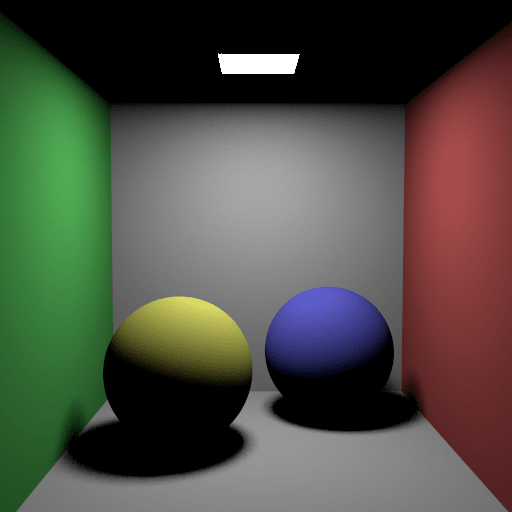
\includegraphics[width=.4\textwidth]{img/1 fundamentals/cb_direct.png}\label{fig:cb_local}}
	\hfill
	\subfloat[]{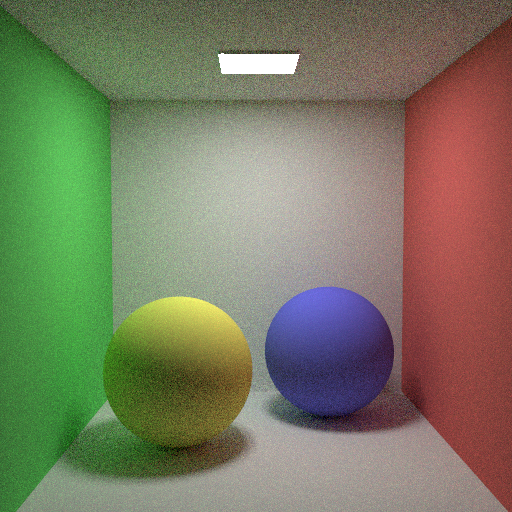
\includegraphics[width=.4\textwidth]{img/1 fundamentals/cb_global.png}\label{fig:cb_global}}
	\caption{The Cornell Box scene with local illumination (Figure \ref{fig:cb_local}) and global illumination (Figure \ref{fig:cb_global}).}
\end{figure}



\subsubsection{Path Tracing}

Multiple approaches for solving the rendering equation exists, for example the \emph{radiosity} method \cite{goral1984modeling}, aiming at solving it via the application of the finite element method. However, the most commonly used methods for solving the rendering equation are Monte Carlo methods. One particular Monte Carlo method is \emph{path tracing}, which is the subject of this section.

\begin{figure}
	\centering
	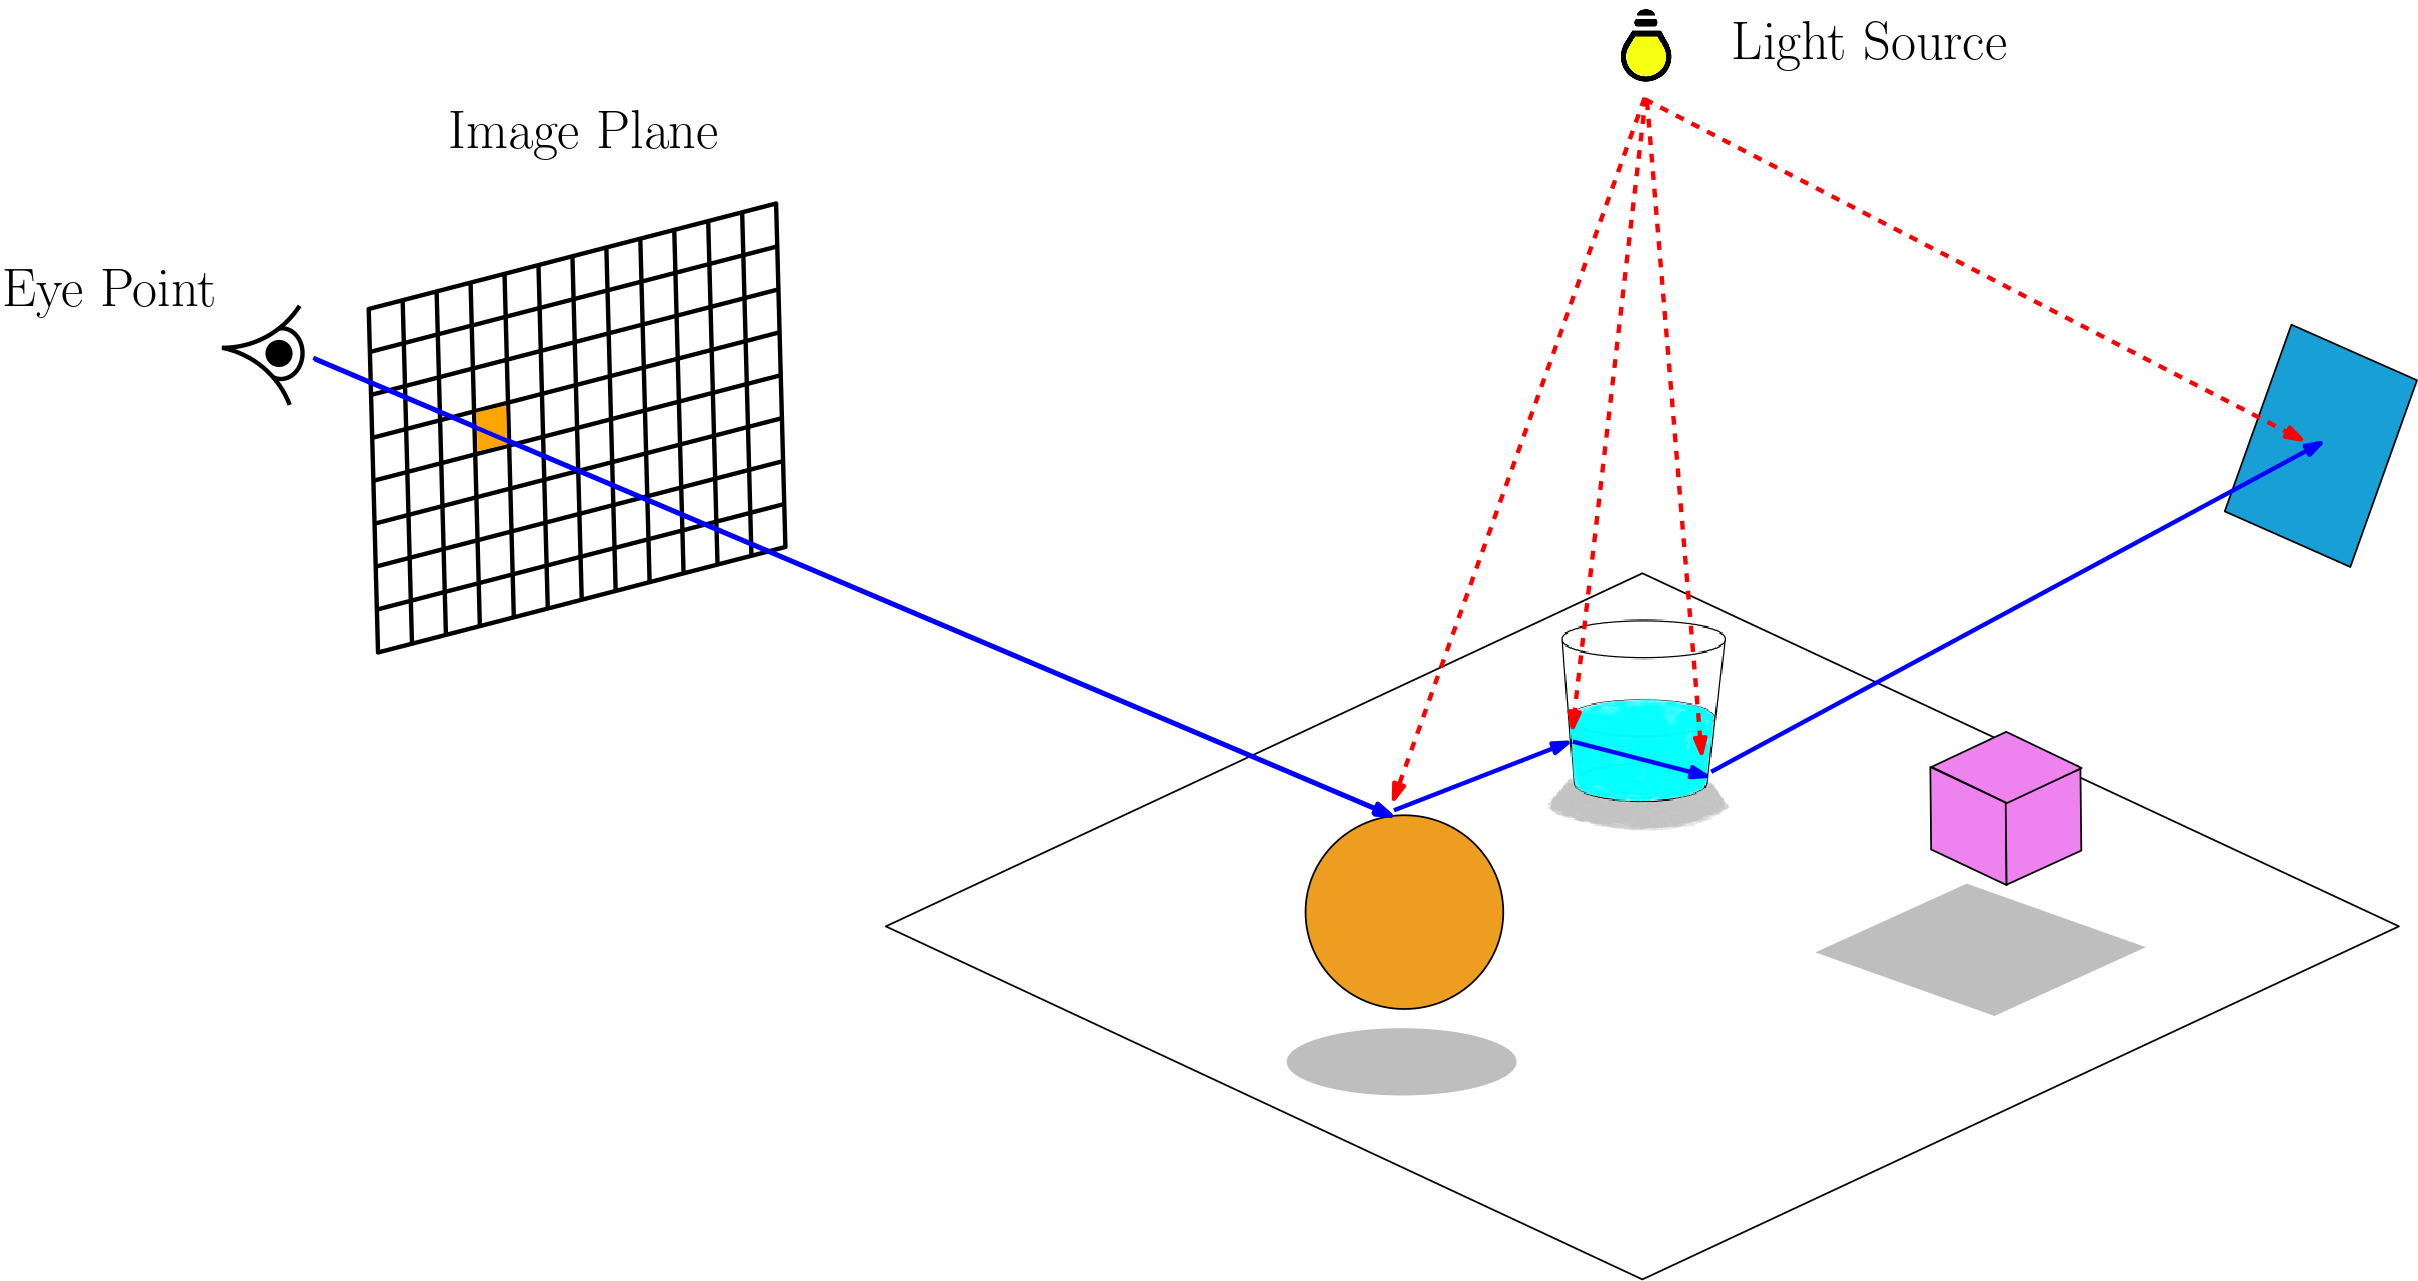
\includegraphics[width=1\linewidth]{img/1 fundamentals/path_tracing.png}
	\caption{Tracing a path for calculating global illumination.}
	\label{fig:pathtracing}
\end{figure}

Path tracing generates "paths" of light rays, starting at the $Eye Point$ and ending at a light source. An example of such path is visualized in Figure \ref{fig:pathtracing}. At each intersection point along the path, the intersected geometries are tested for occlusion and, if the shape is not occluded by another geometry, the direct contribution of the light source(s) are accumulated. 
To prevent the calculations of unprofitable paths, a path is continued according to a so-called "survival probability". This probability can e.g. be formulated as the reflectivity of the surface which is intersected by a ray. If this surface for example reflects only ten percent of light energy, the path is continued with a probability of then percent.
To approximate the integral part of the rendering equation, numerous paths are generated at the intersection point $x$. To generate the final color of the image pixels, the results calculated by the paths are averaged.

\begin{figure}
	\centering
	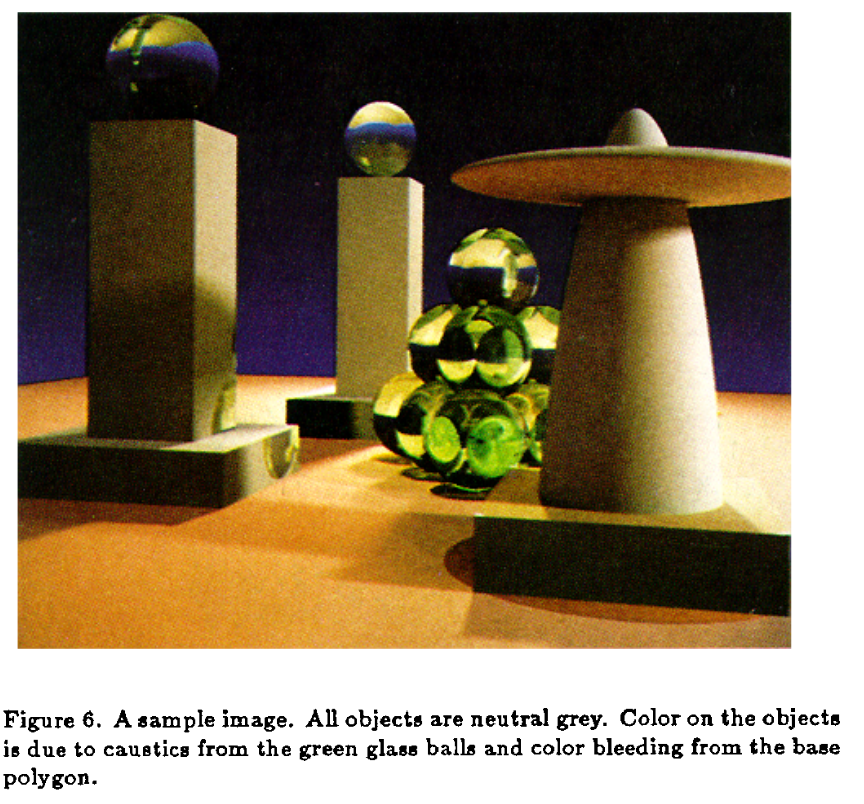
\includegraphics[width=.7\linewidth]{img/1 fundamentals/rendering_eq_figure.png}
	\caption{Original figure from the paper \citetitle{kajiya1986rendering} by Kajiya \cite{kajiya1986rendering}.}
	\label{fig:kajiya_figure}
\end{figure}

With regard to path tracing, we can re-write the rendering equation shown in \ref{eq:renderingeq} in the following way:
\begin{equation}\label{eq:renderingeq_update}
L(x, \omega_{o}) = L_{e}(x, \omega_{o}) \int_{H(x)} L(ray(x, \omega_{i}), -\omega_{i})f_{r}(\omega_{i} \rightarrow \omega_{o})\cos\theta\partial\omega_{i}
\end{equation}

The function $ray(x, \omega_{i})$ recursively calculates the incoming radiance for all directions around the point $x$. A visual result of evaluating this function for each pixel in an image can be seen in Figure \ref{fig:cb_global}.

In comparison of the ray tracing method of \cite{whitted1979improved}, path tracing is capable of simulating advanced optical effects such as soft shadows and diffuse interreflection.

\section{Solid Representations in 3D Space}

A crucial part of ray tracing algorithms is the calculation of intersection points between rays with scene geometry.
The representation of solid objects in the Euclidean space varies, thus does testing them for intersections with given rays. The following section illustrates three types of solid representations in image synthesis environments, such as ART: Analytic surfaces, polygon meshes and constructive solid geometry.

\subsection{Analytical Surfaces}
\label{sec:quadrics}
Analytical surfaces are surfaces in three dimensional Euclidean space, defined by analytic functions. Common analytical surfaces are quadric shapes (or quadrics). Examples of this type of surface representation are spheres, cones, cylinders and paraboloids. The equations describing these shapes can be in implicit form, which has the pleasant property, that testing whether a point $p$ is located at the boundary of such a surface is easy. Generally speaking, implicit equations are relations of the form  $f(x_{0}, x_{1}, ..., x_{n}) = 0$ where $f$ is a function of multiple variables. Consider such a variable as a point $p$ in three dimensional space and evaluated by function $f$. An evaluation of $f$ will result in two possible outcomes: either $f(p) = 0$, which means $p$ is located on the surface of the shape, or  $f(p) \ne 0$, which means the opposite.
Due to this evaluation, quadrics are well suited for intersection testing during ray tracing.
In the following we will provide an example of an intersection calculation between a given unit sphere $S$ with radius $1$ and a given ray $R$. 

\begin{figure}[h]
	\centering
	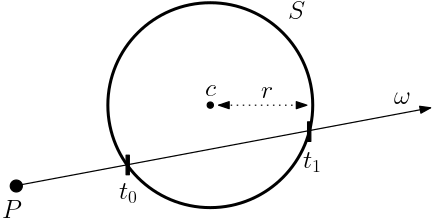
\includegraphics[width=.5\linewidth]{img/1 fundamentals/sphere_isect.png}
	\caption{Intersection between a sphere $S$ with its center point $c$ and radius $r$, and a ray with origin $P$ and direction $\omega$. We attempt to solve a quadradic equation in oder to obtain points $t_{0}$ and $t_{1}$. For reasons of simplicity, visualized in two dimensional space.} 
	\label{fig:sphere_isect}
\end{figure}

The sphere $S$ is implicitly defined by: 
\begin{equation} \label{eq:sphere}
S(x,y,z) = x^{2}+y^{2}+z^{2}-1 = 0
\end{equation}
The ray $R$ in its parametric form is defined by:
\begin{equation}\label{eq:ray}
R(t) = P + t\omega
\end{equation}

\noindent where
\begin{itemize}
	\setlength\itemsep{0.05em}
	\item  $P$ is the origin of ray $R$, a point in Euclidean space,
	\item  $t$ a scalar, and
	\item  $\omega$ the direction vector of $R$.
\end{itemize}

To obtain the two intersection points, the parametric equation defining $R$ is substituted into the implicit equation defining $S$
\begin{equation}\label{eq:substitution}
(P_{x}+t\omega_{x})^{2}+(P_{y}+t\omega_{y})^{2}+(P_{z}+t\omega_{z})^{2}-1 = 0
\end{equation}
and then, since all variables with the exception of $t$ are known, solved for $t$.
Once the two resulting values $t_{0}$ and $t_{1}$ are obtained, the two intersection points $I_{0}$ and $I_{1}$ can be expressed as $I_{0} = P + t_{0}\omega$, and respectively $I_{1} = P + t_{1}\omega$.

\subsection{Polygon Meshes}

Polygon meshes represent shapes as a composition of multiple smaller polygons that are connected with each other via shared edges. The higher the number of such polygons the mesh exhibits, the higher the accuracy of the approximation of the represented shape. The most common types of polygons used are triangles and quadrangles. An example of a representation of a shape with a triangle mesh can be seen in Figure \ref{fig:poly_mesh}. These polygons are composed of a list of vertices, a list of edges connecting these vertices and a face, the area bounded by the vertices and edges. This information is sufficient to describe a polygon in 3D space. A reason why triangles are the most commonly used polygon for meshes is the efficient storage in memory and the property that the vertices of a triangle can never be not co-planar.

\begin{figure}
	\centering
	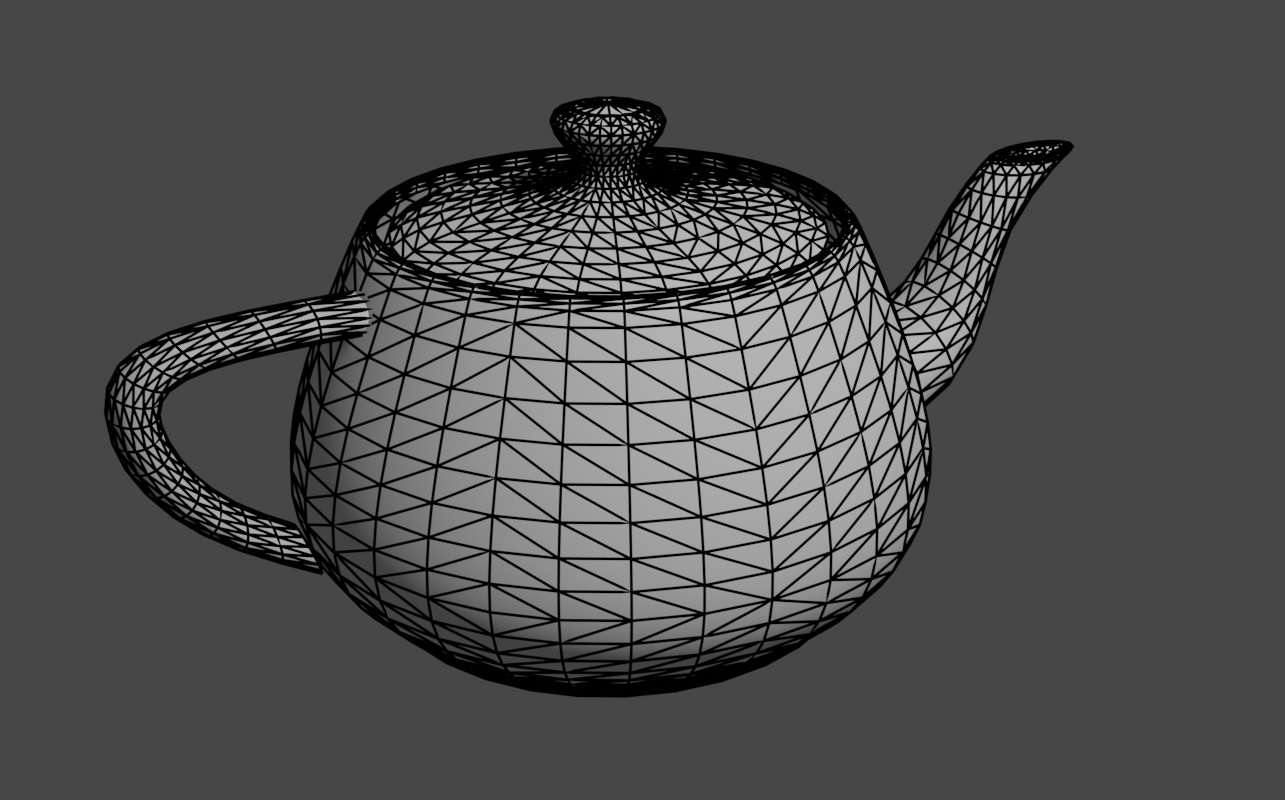
\includegraphics[width=.8\linewidth]{img/1 fundamentals/poly_mesh.png}
	\caption{Polygon mesh of the famous Utah Teapot, rendered with Blender \cite{blender2018}}
	\label{fig:poly_mesh}
\end{figure}

Various ray primitive intersection algorithms exist, for example the Möller– Trumbore intersection algorithm \cite{moller1997fast} for intersecting triangles. In order to test a given ray for intersection with a polygon mesh, theoretically all polygons contained in the mesh in question must be tested for intersection. This is of course a naive approach, since the number of intersection tests that need to be performed is linear in the number of polygons. As such polygon meshes are often composed of several thousand polygons, and testing them all for intersection has a decisive influence on the performance of the rendering process. Section \ref{sec:acceleration} introduces acceleration data structures, aiming at the minimization of those intersection tests.

\subsection{Constructive Solid Geometry (CSG)}

The idea behind constructive solid geometry (CSG) modeling is the application of boolean set operations to geometry primitives in order to create more complex geometries. The boolean set operators are union (logical \texttt{OR}), intersection (logical \texttt{AND}) and difference (denoted as \texttt{SUB}-operator). 
Primitives are usually quadric surfaces such as spheres, cones and cylinders, however, polygon meshes can be regarded as CSG primitives, too. Figure \ref{fig:csg} shows the application of each boolean operator to two sphere primitives. Multiple of such set operations can be hierarchically ordered with the help of a binary tree structure, called the CSG-tree.   

\begin{figure} 
	\centering
	\subfloat[Union of two spheres (\texttt{OR} operator).]{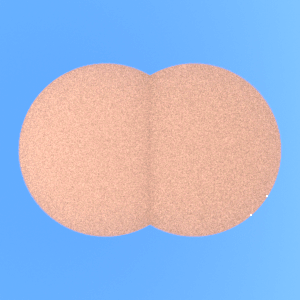
\includegraphics[width=.3\textwidth]{img/1 fundamentals/or.png}\label{fig:csg_or}}
	\hfill
	\subfloat[Intersection of two spheres (\texttt{AND} operator).]{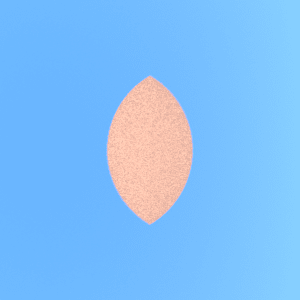
\includegraphics[width=.3\textwidth]{img/1 fundamentals/and.png}\label{fig:csg_and}}
	\hfill
	\subfloat[Left sphere with the right sphere "subtracted" from it (\texttt{SUB} operator).]{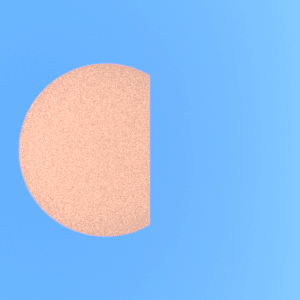
\includegraphics[width=.3\textwidth]{img/1 fundamentals/sub.png}\label{fig:csg_sub}}
	\caption{Boolean operators Union (\ref{fig:csg_or}), Intersection (\ref{fig:csg_and}) and Difference (\ref{fig:csg_sub}) applied to two sphere objects.}
	\label{fig:csg}
\end{figure}

One example of such CSG tree is provided in Figure \ref{fig:csg_tree}. Its leafs are associated with the geometry primitives, the nodes with the set operations. Due to the possibility that two primitives can be translated, rotated or scaled before a boolean operator is applied to them, edges of the tree are associated with transformation information (this is denoted in the figure with the matrix icon). The transformation corresponding to an edge between a node and a node's parent can be "empty", meaning that it has no effect on the primitive represented by that node.  

\begin{figure}
	\centering
	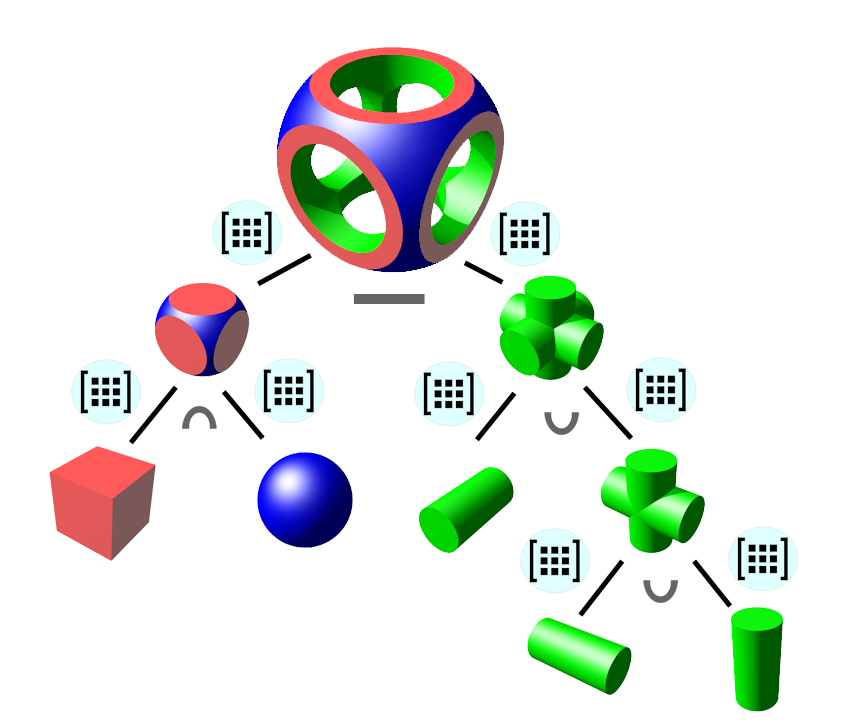
\includegraphics[width=.9\linewidth]{img/1 fundamentals/csg_tree.png}
	\caption{Visualization of a CSG tree hierarchy, originally created by \cite{csgtree} and updated
	with a matrix icon symbolizing affine transformations of geometries.}
	\label{fig:csg_tree}
\end{figure}

\subsubsection{Ray Tracing with CSG}

The ray tracing of CSG was pioneered by \cite{roth1982ray}. In the algorithm, described in the paper \citetitle{roth1982ray}, the intersection calculation for a given ray during the ray tracing process is straightforward: 
All the primitives associated with the leaves of the CSG tree are tested for intersection. If an intersection test with a quadric shape for instance has a positive result, usually two intersection points are calculated: one point when the ray enters the primitive and one point when it exits it (there is the edge case that there exists infinitely many intersection points between a ray and a primitive when the ray is tangent to the primitive, however, this is seldom the case and can be safely ignored). \todo{fucking fix this sentence}Then the CSG tree is traversed bottom up, and each time an interior node, representing a boolean set operator, is encountered, the intersection points of the ray with the primitives associated with the child nodes are evaluated and re-arranged. For example, when considering the \texttt{OR} operator in Figure \ref{fig:csg_or}, and given that a single ray would intersect both spheres, there would be four intersection points: One entering the first sphere, followed by one entering the second sphere, then one exiting the first sphere, and finally one intersection point exiting the second sphere. The \texttt{OR} operator would treat the two spheres as one single object and therefore discard the interior intersection points. Similarly, the \texttt{AND} operator in Figure \ref{fig:csg_and} would discard the two intersections at the exterior of the spheres and keep the two intersections contained in both spheres.
And finally, the \texttt{SUB} operator in Figure \ref{fig:csg_sub} discards every intersection point on the sphere (exterior or interior) that is "subtracted" from the sphere on the left.
\todo{fucking fix this explanation}

The representation of CSG offers one significant advantage: Complex geometry can be expressed via the composition of a manageable amount of primitive shapes, as opposed to large numbers of polygons in a polygon mesh. Because testing whether a point lies inside or outside a primitive is easy, as noted in Section \ref{sec:quadrics}, and since the number of primitives of a composed CSG is usually lower than the amount of polygons in a polygon mesh, the number of intersection tests in each render pass is comparatively low.

Although the CSG modeling technique is several years old, it is still used in practice today, e.g. for computer-aided design.


\section{Spacial Acceleration Data Structures} \label{sec:acceleration}
The computational cost associated with ray tracing and path tracing algorithms has always been regarded as a "necessary evil" one has to face when desiring highly realistic images. An often cited fact is Whitted's observation, that, for complex scenes, 95 percent of the time used by his algorithm is spend on intersection calculations \cite[p 349]{whitted1979improved}. To give an example, the image displayed in Figure \ref{fig:kajiya_figure} was rendered via path tracing on an IBM 3081 machine during 1221 minutes \cite[p 149]{kajiya1986rendering}. The image had a resolution of 512 by 512 pixels and was rendered with 40 paths per pixel.

It was only a logical consequence, that over time, new ideas were introduced for accelerating the ray tracing process. Attempts can be the minimization of the number of rays that are cast into the scene, the development of faster intersection testing algorithms or the minimization of ray-primitive intersection tests. The upcoming of ray acceleration data structures intended to address the later problem. By utilizing these structures, one essentially trades a decrease of the time needed to perform intersection testing for an increase of storage space. The following section focuses on two popular acceleration data structures commonly used: Bounding volume hierarchies and KD trees.

\subsection{Bounding Volume Hierarchy}

Bounding volume hierarchies (BVHs), being introduced by \cite{rubin19803}, are a hierarchical structures of so called \emph{bounding volumes}, aiming at the reduction of unnecessary intersection tests. The idea behind bounding volumes is the enclosure of geometry with an analytical shape, such as a sphere, a cylinder or a box. As previously discussed in Section \ref{sec:quadrics}, testing for an intersection between a given ray and one such analytical shape is easy. If no intersection with such volume is found, this concludes that an intersection between the ray and the enclosed geometry is not possible. Therefore, the intersection calculation between the ray and the enclosed geometry can be safely disregarded. 

\begin{figure}
	\centering
	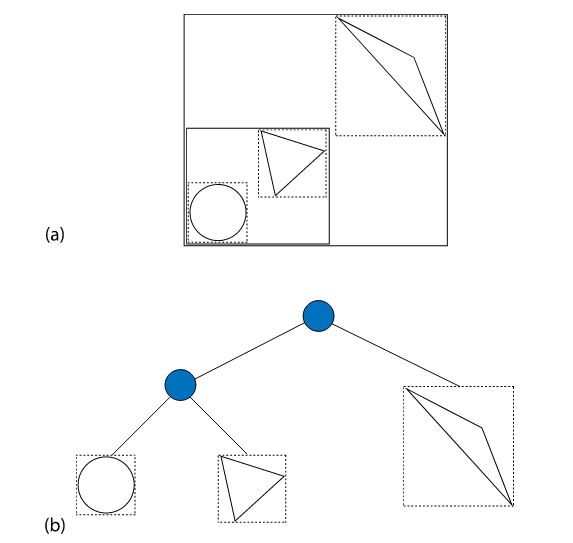
\includegraphics[width=.7\linewidth]{img/1 fundamentals/bvh.png}
	\caption{2D example of a bounding volume hierarchy, taken from \cite{pharr2016physically}. (a) represents the scene, consiting of simple shapes and their axis aligned bounding boxes and (b) the BVH tree structure associated with the scene from (a).}
	\label{fig:bvh}
\end{figure}

Bounding volumes should ideally be chosen, such that they fit the underlying geometry as close as possible in order to further reduce the number of unnecessary intersection test. However, a most commonly used volume is an \emph{axis aligned bounding box}, a hyperrectangle whose sides are parallel to the axis of the coordinate system. Such boxes might not enclose the geometry as tightly as possible, on the other side, testing for intersection becomes computationally cheap and not much memory is needed to store them.

These bounding volumes again can be enclosed in a bounding volume, and thus, complex hierarchies of bounding volumes can be formed.
A BVH then is a hierarchy of multiple of such bounding volumes, stored in a tree structure (commonly in binary trees). In the tree, the leafs represent the bounding boxes of the geometry primitives and the interior nodes are associated with bounding volumes enclosing the node's children. An example of such a tree structure is given by Figure \ref{fig:bvh}. The root of a BVH is typically a bounding box, enclosing the entire virtual scene.

Binary BVHs exhibit some convenient properties: \todo{fucking, check this dude! could be plain wrong} Every geometrical primitive is present in exactly one bounding box, and these bounding boxes do not overlap with each other. Thus, no primitive is possibly tested for intersection twice (unlike with KD trees, which are the subject of the next section). Furthermore, the amount of memory needed for storing a binary BVH is bounded. A BVH that is build over $n$ primitives obtains $2n-1$ total nodes, $n$ leave nodes and $n-1$ interior nodes \cite{pharr2016physically}. 

During ray tracing, the BVH is traversed and a cast ray is tested for intersection between a bounding box that is associated with the current tree node. If an intersection is found, the traversal continues in the node's children, otherwise traversing the sub tree rooted at that node is disregarded.

When compared to KD trees, BVHs usually require more time to be built, however, the ray-primitive-intersection testing is slightly faster. 

\subsection{KD Trees}

\begin{figure}
	\centering
	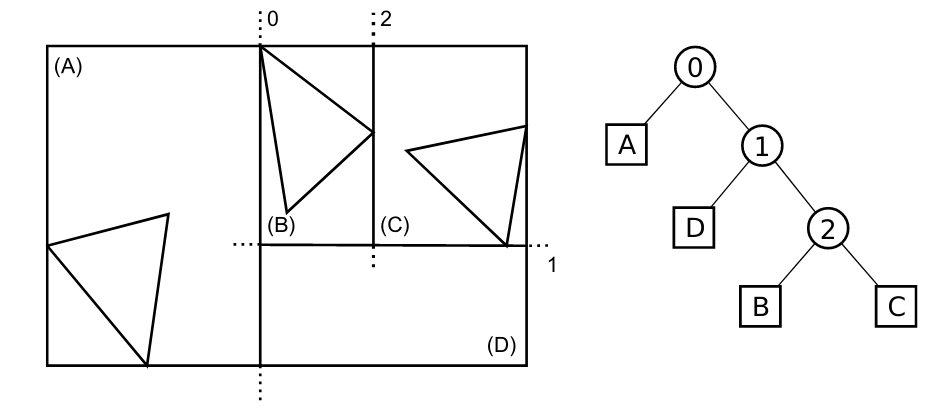
\includegraphics[width=1\linewidth]{img/1 fundamentals/kd_tree.png}
	\caption{Partition of a 2D scene in sub spaces A, B, C, and D with planes 0, 1, and 2. This figure is taken from \cite{hapala2011kd}.}
	\label{fig:kdtree}
\end{figure}

\emph{K-dimensional trees} (or KD trees), which were introduced by \cite{bentley1975multidimensional}, belong to the group of binary space partitioning trees (BSP trees). BSP trees recursively subdivide $k$ dimensional space with $k-1$ dimensional hyperplanes. One subdivision of space takes place when the number of geometric primitives contained in it are greater than a specified threshold. When one such subdivision happens, the space is divided into two smaller half-spaces for which this procedure is repeated until the number of primitives contained in a subdivided area is smaller or equal than the threshold. The hyperplanes that partition space are stored in a binary tree structure. The root of the tree is associated with the hyperplane splitting the bounding volume of the entire scene. Its children to the left are the hyperlanes and primitives in one half-plane that particular plane, and the children to the right are the planes and primitives that are located on the other one. The leaf nodes resemble a list of primitives being located in the area defined by their parent node's hyperplanes.

KD trees are a specialized case where the split-planes are perpendicular to one of the coordinate axis. During the recursive splitting, the axis to which the current plane is perpendicular to, is alternated. This allows for KD trees being efficiently constructed. However, \todo{check this too!} unlike with BVHs, primitives can be located in overlapping sub spaces, therefore intersection points may be calculated twice during ray tracing. 

When being compared to BVHs, the construction is faster (construction methods taking $O(n\log n)$ time exists \cite{wald2001interactive}.)

\section{Intel\textregistered's Embree Framework}
In spite the affect of various ray acceleration data structures and hardware optimizations, exploiting the full capabilities of modern CPUs, which exhibit different architectures and instruction sets and support different algorithms and data structures, remains challenging for ray tracing applications. 

Embree is a high performance rendering framework written in \texttt{C99} which addresses this problem. It offers a collection of vectorized kernels, being optimized for the communication with CPUs that support SSE, AVX, AVX2, AVX-512 and instruction sets. The provided kernels offer a variety of components, e.g. different types of BVHs, traversal algorithms and intersection algorithms, Figure \ref{fig:embree} provides an overview.
During a rendering process, Embree will decide on which components to use for building the acceleration structure and traversing it based information provided by the user and on the target CPU architecture. The later is performed by the "Ray Tracing Kernel Selection" layer of the hierarchy shown in Figure \ref{fig:embree}.

Interesting features of Embree are:
\begin{itemize}
	\setlength\itemsep{0.05em}
	\item 	Finding of the closest hit point, or alternatively any hit point,
	\item 	support for the cast of single rays, ray packets containing 4, 8 or 16 rays, and so-called ray streams of any desired number of rays,
	\item 	high-quality BVH builders,
	\item 	support for the Intel SPMD Program Compiler (ISPC) and the Intel Threading Building Blocks (TBB), and
	\item 	independence from any other graphics API such as OpenGL or DirectX
\end{itemize}

An API for the integration into existing rendering systems is provided and described in a detailed documentation \cite{embree2021Doc}. This documentation furthermore offers tutorial for the familiarization of the framework to new users. The name of the functions belonging to this API are preceded by the abbreviation \texttt{rtc} ("ray tracing kernels"), data types have the abbreviation \texttt{RTC} predeceasing their name. For example the variable \texttt{RTCScene} stores the virtual scene for Embree, and the function \texttt{rtcIntersect1()} performs the intersection testing with a single ray.

\begin{figure}
	\centering
	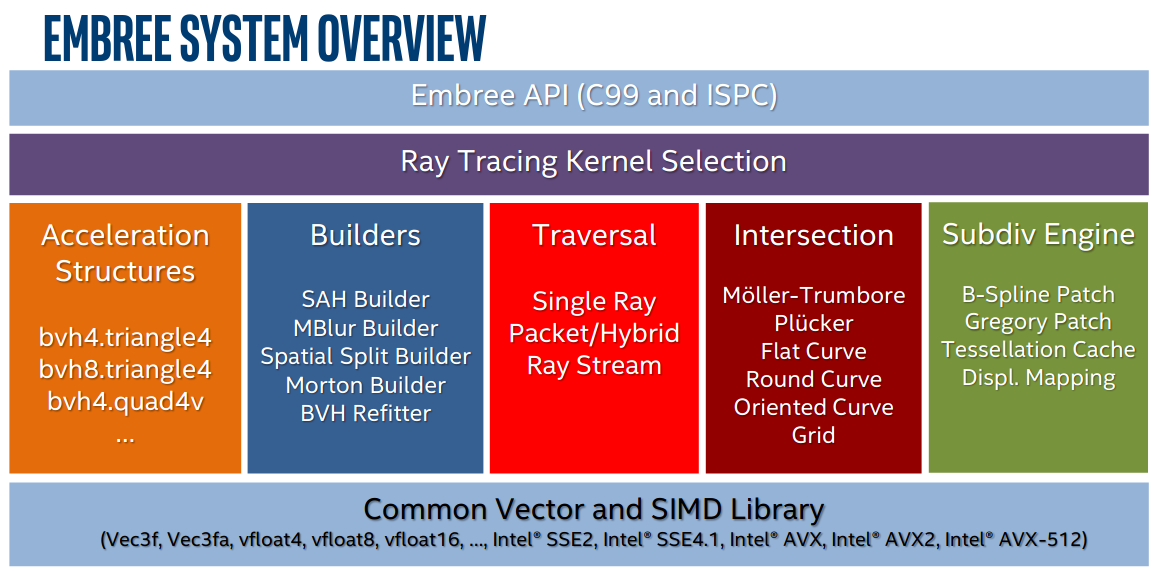
\includegraphics[width=1\linewidth]{img/1 fundamentals/embree_overview.png}
	\caption{System overview of Embree, taken from the SIGGRAPH presentation \citetitle{embreeSlides} \cite{embreeSlides}.}
	\label{fig:embree}
\end{figure}

Embree supports a variety of geometric shapes such as triangles, quads, and certain types of curves, such as Bézier curves, B-Splines and Catmull-Rom-Splines.
Another notable feature of Embree is the support of custom geometries. These will be referred to as \emph{User defined geometries}. 

Embree is open source, and therefore publicly available. Supported platforms are (32-bit and 64-bit), Linux (64-bit), and macOS (64-bit). The latest version of Embree at the time of writing this thesis is 3.13.0. 

\subsubsection{Ray Tracing in Embree}
Embree follows a device concept, allowing for the use of the Embree API by different components of the image synthesis application without interfering each other. An \texttt{RTCDevice} can be created with the function \texttt{rtcNewDevice} and released via the function \texttt{rtcReleaseDevice}. Such device types are used by Embree to create further components, such as virtual scenes which serve as the container for various scene geometry. A scene in Embree, represented by the data type \texttt{RTCScene}, can be created via the function \texttt{rtcNewScene}, to which the \texttt{RTCDevice} is passed to as an argument, and released via the function \texttt{rtcReleaseScene}. Different geometries can be attached or detached by the functions \texttt{rtcAttachGeometry}, which will furthermore assign a unique ID to the geometry, and \texttt{rtcDetachGeometry}. Once an \texttt{RTCGeometry} is attached to the \texttt{RTCScene}, it can be released via the call of the function \texttt{rtcReleaseGeometry}.
After the attachment of the complete scene geometry, the scene can be committed by calling the function \texttt{rtcCommitScene} in order to trigger the creation of Embree's internal acceleration structures. After the invocation of this function, the individual geometries cannot be edited or manipulated.

Geometries in Embree are represented by a \texttt{RTCGeometry} data type. These types can be created with the function \texttt{rtcNewGeometry} which takes the \texttt{RTCDevice} and an enum specifying the geometry type (e.g. triangle, quad, user defined geometry) as input parameters. In case the geometry being a triangle, quadrangle or a type of curve, so-called \emph{geometry buffers} can be created and linked to the \texttt{RTCGeometry} by invoking the function \texttt{rtcSetNewGeometryBuffer}. These buffers will store information such as vertices, indices and surface normals of the geometry.  

In order to initialize a user defined geometry, one has to provide a function for calculating the bounding box for the geometry, a function for intersection testing and another function for occlusion testings. These functions are passed to Embree as callback functions. Furthermore, the number of geometric primitives, which together compose the geometry, has to be set, and a so-called \emph{User data pointer} associated with the geometry. A user data pointer points to the representation of the geometry by the rendering application in memory. In the interior of the callback function for calculating the intersection with the user defined geometry, the original representation of the geometry can be easily retrieved via this pointer. The passing of the various callback functions to Embree is done via invocation of the functions \texttt{rtcSetGeometryUserPrimitiveCount}, \texttt{rtcSetGeometryUserData}, \texttt{rtcSetGeometryBoundsFunction}, \texttt{rtcSetGeometryIntersectFunction}, \newline and \texttt{rtcSetGeometryOccludedFunction}.

Once the \texttt{RTCDevice} and the \texttt{RTCScene} are set up, the scene geometry is attached to the \texttt{RTCScene}, and the internal acceleration data structures have been built, nothing stands in the way of performing the actual ray tracing with Embree. 

In the following example, only ray tracing with single rays as opposed to packet ray tracing is considered. We will furthermore not consider instancing, due to the reason that this feature does not find use in the work of this thesis.

In order to ray trace a virtual scene, a per ray query intersection context, \texttt{RTCIntersectContext}, has to be set up via the function \texttt{rtcInitIntersectContext}. This structure is used for the configuration of intersection flags, among other things. 
Subsequently, a \texttt{RTCRayHit} struct is declared. This struct is composed of an \texttt{RTCRay} struct, abstracting the ray that is used by Embree to preform the intersection testing, and an \texttt{RTCHit} struct, in which information concerning the intersection point, such as the surface normal, the barycentric UV coordinates of the point, and the geometry ID associated with the intersected geometry are stored.
The \texttt{RTCRay} struct stores the ray orientation and direction, so-called \texttt{tnear} and \texttt{tfar} values, indicating the boundaries of a range of possible hit distances, and other information such as an id for the ray, a ray mask and a \texttt{time} value useful when motion blur is desired.
When the target ray tracing application is generating a ray, the values of the \texttt{RTCRay} struct are updated with the ray orientation and direction. The \texttt{tnear} value is usually set to zero and the \texttt{tfar} value is set to infinity. The geometry ID of the \texttt{RTCHit} struct is initialized with the macro \texttt{RTC\_INVALID\_GEOMETRY\_ID}.

After the \texttt{RTCIntersectContext} and the \texttt{RTCRayHit} structs have been successfully initialized and updated, the ray-primitive intersection testing is performed via invocation of the function \texttt{rtcIntersect1} to which the \texttt{RTCScene}, a reference to both the \texttt{RTCIntersectContext} and the \texttt{RTCRayHit} are passed as arguments. In case of a found intersection, this function will update the \texttt{tfar} value of the \texttt{RTCRay} with the closest hit distance and the geometry ID of the \texttt{RTCHit} with the geometry ID associated to the intersected geometry.

In case of performing intersection testing between a user defined geometry and a ray, these values have to be updated manually inside the intersection function that was passed to Embree as a callback function.

When the intersecting testing procedure has finished, the geometry ID of the \texttt{RTCHit} will give insight on whether an intersection was found or not. If the value of this variable remains \texttt{RTC\_INVALID\_GEOMETRY\_ID}, one can conclude that no intersection was found. Otherwise, an intersection was found and the \texttt{RTCRay} and \texttt{RTCHit} components of the \texttt{RTCRayHit} will provide the hit distance, the coordinates of the surface normal at the intersection point and the UV coordinates of the intersection point.
\chapter{Technical details regarding Embree and ART (WT)}

Some introduction stuff.¸ \todo{do}

\section{A brief introduction to ART}
\label{chap:art}

The Advanced Rendering Toolkit (ART), serves as the environment in which Embree shall be integrated into. Therefore, this chapter provides a brief introduction to ART to familiarize the reader with its core mechanics. Apart from a short description of the general workflow of ART, only its aspects that are relevant for the integration of Embree are considered in this chapter. For a more detailed description of ART and the scene description language, we would like to refer the reader to the ART Handbook \cite{arthandbook} and the ARM File Reference Manual \cite{artreferencemanual}.\footnote{It should be mentioned here that at the time of writing this thesis, both documents are still work in progress, and therefore incomplete. However, they will be expanded in the future.}

The latest version of ART at the time of writing this thesis is Version 2.0.3.


\subsection{Purpose and features}

As indicated in the introduction, ART considers its target audience computer graphics researchers who are interested in the field of predictive rendering. Predictive rendering is a branch of the computer graphics field that is dedicated to the research of light transport simulation, with which one can accurately predict the appearance of tan object or a virtual scene under different viewing conditions (compare \cite{wilkie2009predictive}.) \todo{use Alban's example} While the purpose of "conventional rendering" (to which we count the rendering procedures encountered in Chapter \ref{chap:fundamentals}) lies in the creation of "believable" imagery to create a certain impression to an observer, predictive rendering is concerned with the synthesis of radiometrically correct images, which serve as matters of conducting actual research as opposed to communicating a visual impression on an observer.

ART offers a variety of important features for predictive rendering that are currently non-standard in other "mainstream" rendering systems, such as polarization visualization support, the physically plausible handling of fluorescent materials \cite{mojzik2018handling}, and the enabling of spectral rendering. For the later, ART implements the "Hero wavelength spectral sampling" technique \cite{wilkie2014hero} and utilizes its own spectral image file format. Additionally, various research projects belonging to the "Sky Dome Appearance Project" are implemented in ART \cite{hosek2012analytic, hovsek2013adding, wilkie2013predicting}.


\subsection{Overview}
ART	is composed of a number of UNIX-like-command line applications (therefore the name Advanced Rendering \emph{Toolkit}). The applications are written in \texttt{C} and \texttt{Objective-C}. 

In the following, we provide an overview over the individual applications contained in the toolkit:
\begin{description}
	% \setlength\itemsep{0.05em}
	\item[\emph{artist}] \hfil \\ This is the actual command-line application renderer, taking an ARM scene file as input and storing the raw information gathered by path tracing process in an intermediate file described in a proprietary file format. This file is not an image file one can display in an image viewing application.
	\item[\emph{tonemap}] \hfil \\ This tool can be used for tone-mapping the (possibly spectral) information stored in the file being created by \texttt{artist} in order to obtain viewable results.
	\item[\emph{bugblatter}] \hfil \\ This application creates difference images of two provided, same-sized images. These difference images can be useful when debugging computer graphics applications.
	\item[\emph{polvis}] \hfil \\ Since ART supports rendering polarization effects by storing the amount of polarized light per pixel in each pixel of a spectral image, these polarization effects can be visualized by the use of this tool.
	\item[\emph{impresario}] \hfil \\ With this application it is possible to store and display intermediate rendering results from currently running rendering jobs. This application is similar to a software daemon.
\end{description}

For our integration of Embree, the only relevant application is \texttt{artist}. 

In order to successfully render an image with \texttt{artist}, in the ARM scene file, one has to at least provide a virtual camera, the scene geometry, and an action sequence. An action sequence is a user defined procedure, telling ART how to render the provided scene. Functionality of other applications like \texttt{tonemap} or \texttt{polvis} can be included in an action sequence.
In order to execute the individual steps  defined by an action sequence (which are referred to as \emph{actions}), ART makes use of a single stack data structure. During the execution of one such action, one or multiple data objects are taken off the stack, manipulated according to the action in question, and placed back on the stack. One example of such an action would be the creation of axis aligned bounding boxes for each object present in the scene. Here, the scene graph object is popped from the stack, bounding boxed are calculated for each geometry, then these boxes are inserted into the scene graph. Further bounding boxes, enclosing these for the geometries are calculated and inserted into the scene graph, too. Finally, the manipulated scene graph is pushed back to the stack.

Another noteworthy detail to mention is the ability of ART to utilize multiple available processor cores to perform a rendering job. By default, ART determines the number of available cores before the path tracing, however, a number of a desired amount of cores to perform the rendering job can be provided by invoking

\begin{Verbatim}
artist foo.arm -j<n>
\end{Verbatim}

where \texttt{<n>} is the number of preferable cores.

To achieve lock free parallelism between the individual threads, the scene graph is copied and one such copy is assigned to each thread. 
 

\subsection{Scene graph infrastructure}
Some popular rendering systems (among them Mitsuba 2 and pbrt) describe a virtual scene in the following way: A virtual scene, abstracted by a \texttt{Scene} class object, obtains a collection of geometric shapes. These shapes are represented by a \texttt{Shape} base class, which offers functions for calculating its bounding box and performing intersection tests with a given ray. Various shape types can be represented as a child classes of this \texttt{Shape} class. This is an ideal design for Embree since these shapes can be initialized as User Defined Geometries. Once Embree finds an intersection with a bounding box of a particular shape, its representation in memory can be retrieved via the User pointer \todo{explain} and an instance function of the \texttt{Shape} class for ray-intersection testing can be called. 

\begin{figure}
	\centering
	
	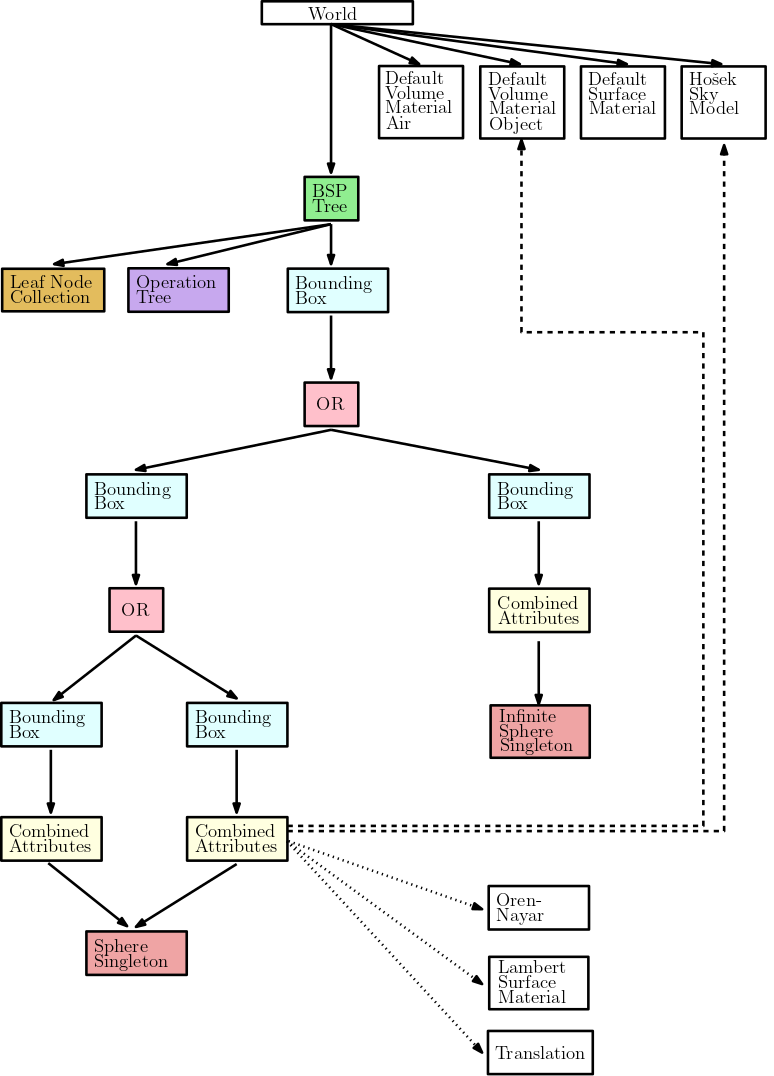
\includegraphics[width=1\linewidth]{img/2 art/scene_graph.png}
	\caption{Scene graph used to render Figure \ref{fig:csg_or}. In this graph, bounding boxes have already been inserted and a KD tree was built over the scene.} 
	\label{fig:scene_graph}
\end{figure}

\begin{table}
  \centering
  {\footnotesize
    \begin{tabular}{m{3cm}m{8cm}}
      \toprule
      Scene graph node & Function  \\
      \midrule
      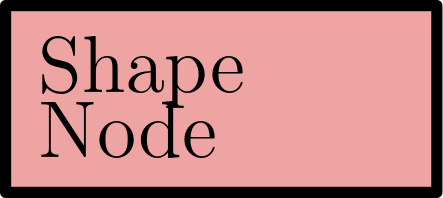
\includegraphics[scale=0.5]{img/2 art/shape_node.png} & This node belongs
                                                              to the category of
                                                              "shape nodes" that
                                                              are associated
                                                              with the
                                                              representation of
                                                              a geometry by
                                                              ART. Nodes of this
                                                              type are always
                                                              leafs.\\
      \midrule
      
\includegraphics[scale=0.5]{img/2 art/comb_attr_node.png} & This node is
      \\
      \midrule
    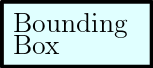
\includegraphics[scale=0.5]{img/2 art/bounding_box.png} & This node
                                                                       represents
                                                                       a
                                                                       bounding
                                                                       box,
                                                                       enclosing
                                                                       the
                                                                       components
                                                                       of the
                                                                       sub tree
                                                                       rooted at
                                                                       the
                                                                       node. \\
      \midrule
     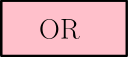
\includegraphics[scale=0.5]{img/2 art/or.png} & Nodes with two
                                                              children,
                                                              representing the
                                                              primitives to
                                                              which this CSG
                                                              operation is
                                                              applied to (in
                                                              this example, it
                                                              the two nodes are
                                                              representing the
                                                              union
                                                              operation). \\
      \midrule
     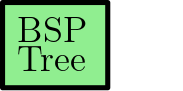
\includegraphics[scale=0.5]{img/2 art/bsp_node.png} & Represents
                                                                    the KD tree
                                                                    that is
                                                                    build over
                                                                    the
                                                                    scene. Its
                                                                    children are
                                                                    the entire
                                                                    scene
                                                                    geometry, a
      \\
      \bottomrule
    \end{tabular}}
  \caption{Nodes in the scene graph displayed in Figure \ref{fig:scene_graph} and their functionality.}
  \label{tab:nodes}
\end{table}


The scene graph being utilized by ART diverges from this design. This section provides an overview over different nodes in the scene graph and their functionality on the basis of a provided example scene graph. This scene graph, which was used by ART to render the image displayed in Figure \ref{fig:csg_or}, is shown in Figure \ref{fig:scene_graph}. Table \ref{tab:nodes} displays its nodes and a brief description of their functionality and relation to other nodes. However, we will only list nodes for which the comprehension of their functionality is important to follow the implementation description in the next chapter.
On particularity of the scene graph is that it can be utilized by every application mentioned in the previous section, with the exception of \emph{impresario}.

\subsection{Ray Tracing with ART}
\label{sec:art_raytracing}
The functionality redarding ray tracing in ART is abstracted in the \texttt{ArnRayCaster} class. This class is inherited from the \texttt{ArnGraphTraversal} class. 

\todo{talk this over with Alban}

\todo{talk about org scene graph rendering}

\begin{figure}[!tbp]
	\centering
	\subfloat[Image rendered by traversing the KD Tree.]{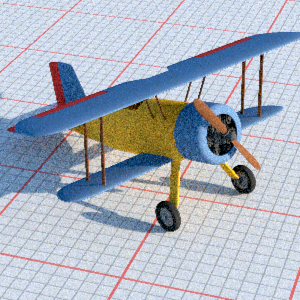
\includegraphics[width=.4\textwidth]{img/2 art/plane.png}}
	\hfill
	\subfloat[Image renderd by traversing the original scene graph.]{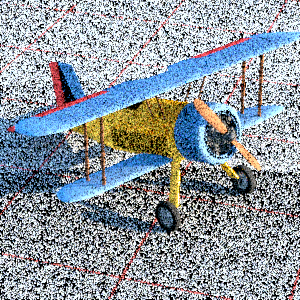
\includegraphics[width=.4\textwidth]{img/2 art/planeArtifacts.png}}
	\caption{Comparison of rendered images by traversing ART's internal KD tree and traversing the original scene graph.}
	\label{fig:org_scenegraph}
\end{figure}

\todo{talk about intersection list}

\section{Ray Tracing with Embree}
\label{sec:embree_raytracing}
Embree follows a device concept, allowing for the use of the Embree API by different components of the image synthesis application without interfering each other. An \texttt{RTCDevice} can be created with the function \texttt{rtcNewDevice} and released via the function \texttt{rtcReleaseDevice}. Such device types are used by Embree to create further components, such as virtual scenes which serve as the container for various scene geometry. A scene in Embree, represented by the data type \texttt{RTCScene}, can be created via the function \texttt{rtcNewScene}, to which the \texttt{RTCDevice} is passed to as an argument, and released via the function \texttt{rtcReleaseScene}. Different geometries can be attached or detached by the functions \texttt{rtcAttachGeometry}, which will furthermore assign a unique ID to the geometry, and \texttt{rtcDetachGeometry}. Once an \texttt{RTCGeometry} is attached to the \texttt{RTCScene}, it can be released via the call of the function \texttt{rtcReleaseGeometry}.
After the attachment of the complete scene geometry, the scene can be committed by calling the function \texttt{rtcCommitScene} in order to trigger the creation of Embree's internal acceleration structures. After the invocation of this function, the individual geometries cannot be edited or manipulated.

Geometries in Embree are represented by a \texttt{RTCGeometry} data type. These types can be created with the function \texttt{rtcNewGeometry} which takes the \texttt{RTCDevice} and an enum specifying the geometry type (e.g. triangle, quad, user defined geometry) as input parameters. In case the geometry being a triangle, quadrangle or a type of curve, so-called \emph{geometry buffers} can be created and linked to the \texttt{RTCGeometry} by invoking the function \texttt{rtcSetNewGeometryBuffer}. These buffers will store information such as vertices, indices and surface normals of the geometry.  

In order to initialize a user defined geometry, one has to provide a function for calculating the bounding box for the geometry, a function for intersection testing and another function for occlusion testings. These functions are passed to Embree as callback functions. Furthermore, the number of geometric primitives, which together compose the geometry, has to be set, and a so-called \emph{User data pointer} associated with the geometry. A user data pointer points to the representation of the geometry by the rendering application in memory. This user data pointer can be associated with geometry types other than user defined geometry.
In the interior of the callback function for calculating the intersection with the user defined geometry, the original representation of the geometry can be easily retrieved via this pointer. The passing of the various callback functions to Embree is done via invocation of the functions \texttt{rtcSetGeometryUserPrimitiveCount}, \texttt{rtcSetGeometryUserData}, \texttt{rtcSetGeometryBoundsFunction}, \texttt{rtcSetGeometryIntersectFunction}, \newline and \texttt{rtcSetGeometryOccludedFunction}.

Once the \texttt{RTCDevice} and the \texttt{RTCScene} are set up, the scene geometry is attached to the \texttt{RTCScene}, and the internal acceleration data structures have been built, nothing stands in the way of performing the actual ray tracing with Embree. 

In the following example, only ray tracing with single rays as opposed to packet ray tracing is considered. We will furthermore not consider instancing, due to the reason that this feature does not find use in the work of this thesis.

In order to ray trace a virtual scene, a per ray query intersection context, \texttt{RTCIntersectContext}, has to be set up via the function \texttt{rtcInitIntersectContext}. This structure is used for the configuration of intersection flags, among other things. 
Subsequently, a \texttt{RTCRayHit} struct is declared. This struct is composed of an \texttt{RTCRay} struct, abstracting the ray that is used by Embree to preform the intersection testing, and an \texttt{RTCHit} struct, in which information concerning the intersection point, such as the surface normal, the barycentric UV coordinates of the point, and the geometry ID associated with the intersected geometry are stored.
The \texttt{RTCRay} struct stores the ray orientation and direction, so-called \texttt{tnear} and \texttt{tfar} values, indicating the boundaries of a range of possible hit distances, and other information such as an id for the ray, a ray mask and a \texttt{time} value useful when motion blur is desired.
When the target ray tracing application is generating a ray, the values of the \texttt{RTCRay} struct are updated with the ray orientation and direction. The \texttt{tnear} value is usually set to zero and the \texttt{tfar} value is set to infinity. The geometry ID of the \texttt{RTCHit} struct is initialized with the macro \texttt{RTC\_INVALID\_GEOMETRY\_ID}.

After the \texttt{RTCIntersectContext} and the \texttt{RTCRayHit} structs have been successfully initialized and updated, the ray-primitive intersection testing is performed via invocation of the function \texttt{rtcIntersect1} to which the \texttt{RTCScene}, a reference to both the \texttt{RTCIntersectContext} and the \texttt{RTCRayHit} are passed as arguments. In case of a found intersection, this function will update the \texttt{tfar} value of the \texttt{RTCRay} with the closest hit distance and the geometry ID of the \texttt{RTCHit} with the geometry ID associated to the intersected geometry.

In case of performing intersection testing between a user defined geometry and a ray, these values have to be updated manually inside the intersection function that was passed to Embree as a callback function.

When the intersecting testing procedure has finished, the geometry ID of the \texttt{RTCHit} will give insight on whether an intersection was found or not. If the value of this variable remains \texttt{RTC\_INVALID\_GEOMETRY\_ID}, one can conclude that no intersection was found. Otherwise, an intersection was found and the \texttt{RTCRay} and \texttt{RTCHit} components of the \texttt{RTCRayHit} will provide the hit distance, the coordinates of the surface normal at the intersection point and the UV coordinates of the intersection point.


% !TeX spellcheck = en_US
\chapter{Integration of Embree into ART}
\label{chap:integration}

The following section outlines our approach to the integration of Embree into ART. The language in which the individual procedures are formulated is Objective-C since the higher-level functionality of ART has been written in this language. The Embree library itself is written in C and intended for the integration into image synthesis environments written in C/C++, which is the industry standard. However, due to Objective-C being a strict superset of C, these two languages can be intermixed seamlessly. Therefore, no issues concerning the cross-linking of C and Objective-C were discovered during the development.

\section{Design choices}

One important design choice was to abstract functionality regarding Embree in a single class, which we gave the name \texttt{ArnEmbree}, conform to the naming convention of Objective-C classes in ART. Classes of type "\texttt{Arn<name>}" belong to the category of so-called "Scene graph classes", to which, according to our own opinion, the \texttt{ArnEmbree} class belongs the closest to.

The main tasks of this class are the creation and deletion of an \texttt{RTCDevice} and an \texttt{RTCScene}, the adding of different scene geometry to the \texttt{RTCScene}, and performing the intersection calculations with Embree. This class will act as a singleton object. To quote from the ART handbook: "Apart from this struct, [the \texttt{art\_gv} global variable]\footnote{The \texttt{art\_gv} is a struct containing information that is globally accessible to the different class objects in ART. For more information on this, we refer to the ART Handbook.} there are no genuine global variables in ART, only global constants" \cite[Chapter 4.1.2]{arthandbook}. The singleton object obviously contradicts this statement. The main reason for this design is to keep the functionality regarding Embree separate from the functionality of what we will from now on referring to as \emph{Native ART}, the original Advanced Rendering Toolkit without Embree integration.

At an early stage of the development of our approach, it was not obvious whether Embree could be integrated into ART at all. If our work on the integration were unsuccessful, this separation would at least ease reverse engineering ART to its original form.
In spite of this separation, an inclusion of the \texttt{ArnEmbree} singleton class to the \texttt{art\_gv} variable is a solvable problem.

Another design decision was to enable support from Embree only when the user provided the parameter flag \texttt{-e} or \texttt{--embree} when invoking \texttt{artist}, like this:

\begin{Verbatim}
$ artist foo_scene.arm -e
\end{Verbatim}

Initially, the provision of a parameter flag was intended for easily switching Embree support on and off to draw comparisons between the performances of ART with and without the help of Embree. However, we kept this functionality because there is one case (revolving around the rendering of CSG composed of triangle meshes) where ray tracing with Embree is inefficient. We will turn to this circumstance in more depth when discussing the results in Chapter \ref{chap:results}. 

Once the command line arguments of \texttt{artist} are evaluated, the \texttt{ArnEmbree} singleton class object, which we gave the name "\texttt{embreeManager}", is initialized and set up, if the parameter flag was set. Otherwise, \texttt{embreeManager} is set to \texttt{NULL}. From this point on, the \text{ArnEmbree} singleton can be retireved from anywhere in the code and at any point of the action sequence by the instruction, shown in Listing \ref{lst:embree_manager}.

\begin{listing} 
	\begin{lstlisting}[caption={Retrieval the \texttt{ArnEmbree} singleton object.}, label={lst:embree_manager}]
	ArnEmbree * embree = [ArnEmbree embreeManager];
	\end{lstlisting}
\end{listing}


\begin{listing}
	\begin{lstlisting}[caption={Verifying if Embree support was enables by the user.}, label={lst:check_embree}]
	 if( [ArnEmbree embreeEnabled] ) 
	 {
	 		// ...
	 }
	\end{lstlisting}
\end{listing}

Furthermore, if the singleton was initialized and set up, another global Boolean variable, indicating whether Embree is enabled or not, is set to \texttt{true}. The value of this Boolean can be retrieved by calling the class method called \texttt{embreeEnabled}. An example of this is given in Listing \ref{lst:check_embree}.

\section{The \texttt{ArnEmbree} class and extension of the \texttt{ArnRayCaster} class}

The \texttt{ArnEmbree} class is constructed the following way: Instance variables are provided to store a single \texttt{RTCDevice} and a single \texttt{RTCScene} for Embree. Although the instantiation of multiple scenes on a single device is possible with Embree, we consider only single scenes containing all scene geometry since ART does not support the instantiation of multiple scenes.

Furthermore, class methods are defined for the initialization of different geometry types for Embree, their attachment to the \texttt{RTCScene}, and finally for committing the \texttt{RTCScene}, which will trigger the build of Embree's internal spatial acceleration data structures. Due to these data structures, the creation of ART's internal KD tree is not necessary and can be discarded.

In order to perform the actual ray-primitive intersection testing with Embree, an instance method was added to the \texttt{ArnRayCaster} class, which we gave the name \texttt{getIntersectionListWithEmbree}. If Embree support is enabled, instead of traversing ART's KD tree, this method is called. In this function, a given ray is converted to an \texttt{RTCRay} and Embree's internal function for intersection testing, \texttt{rtcIntersect1}, is invoked. Since ART only supports the cast of single rays, as opposed to ray packets, functionality for casting ray packets with Embree is not considered. After the intersection testing is performed, the \texttt{tfar} value is updated with the hit distance (which will remain being set to \texttt{INFINITY} if no intersection was found). The UV coordinates, the surface normal at the hit point, and the shape associated with the hit geometry are stored in an intersection list. From this point, the ray tracing process continues as usual until the next ray is cast into the scene.

\section{Initializing shapes for Embree}

ART supports a variety of different geometrical shapes. An overview of these shapes can be found in the ART Scene File Reference Manual. The supported shapes are divided by ART into two categories: \emph{Analytic shapes} and \emph{Simple indexed shapes}. Analytic shapes are represented by ART as outlined in Section \ref{sec:quadrics}. Simple indexed shapes, on the other hand, are described by an array of vertices and indices associated with the shape in question (similar to the triangle primitives in \emph{OpenGL}). In ART, two shapes, namely triangles and quadrangles, are considered simple indexed shapes. Figure \ref{fig:shape_types} shows example shapes belonging to the two categories. 
This section describes the initialization of these shape types for Embree.


\begin{figure}[!tbp]
	\centering
	\subfloat[An example of a simple indexed shape: a triangle.]{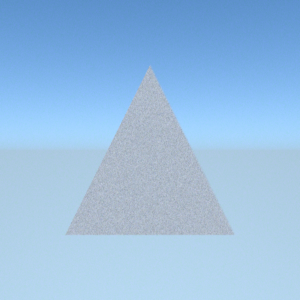
\includegraphics[width=.3\textwidth]{img/3 approach/triangle.png}\label{fig:art_triangle}}
	\hfil
	\subfloat[An example of an alytical shape: a torus aligned on Y-axis.]{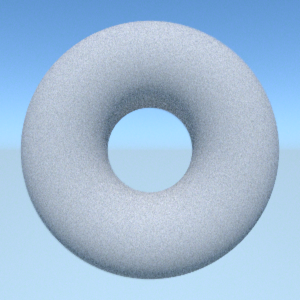
\includegraphics[width=.3\textwidth]{img/3 approach/torus.png}\label{fig:art_torus}}
	\caption{Shape types in ART.}
	\label{fig:shape_types}
\end{figure}

Although it would be convenient to initialize all shapes in ART as user defined geometries for Embree, we make the distinction between \emph{user-defined geometry} and \emph{non-user-defined geometry}.

Into the first category will fall the analytically described shapes. Triangles and quadrangles will be regarded as non user defined geometry and represented by Embree's own primitive types \texttt{RTC\_GEOMETRY\_TYPE\_TRIANGLE} and \texttt{RTC\_GEOMETRY\_TYPE\_QUAD}. This division makes sense since the rendering of these primitive types with Embree is more efficient than the rendering user defined geometries. Furthermore, all the information needed to set up these primitive types is the vertices and indices associated with the shape. They can be easily transferred from ART to Embree. 

\begin{figure} 
	\centering
	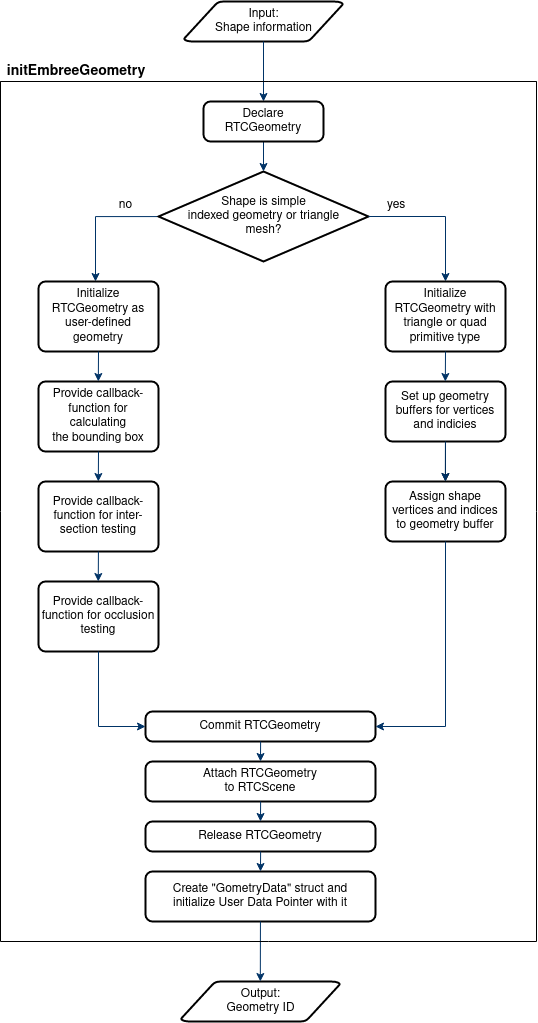
\includegraphics[width=.75\linewidth]{img/3 approach/shape_init_diagram.png}
	\caption{Flowchart describing the workflow of the \texttt{initEmbreeGeometry} function.}
	\label{fig:init_chart}
\end{figure}

The initialization of geometries for Embree takes place during the assembly of the scene graph from the information that has been parsed from the ARM scene file. To be precise, a particular shape is initialized for Embree when the Combined Attributes nodes and Shape nodes associated with it are created and inserted into the scene graph. After this insertion, an instance method of the \texttt{ArnEmbree} class, \texttt{initEmbreeGeometry}, is called. The shape object itself, together with the \texttt{Combined Attributes} object, and the transformation matrix, are passed as function arguments. 
\\

The \texttt{initEmbreeGeometry} function does the following:

\begin{itemize}
	\setlength\itemsep{0.05em}
	
	\item \textbf{Initialization of an \texttt{RTCGeometry}}
	\item[] To initialize a geometry for Embree, an \texttt{RTCGeometry} needs to be created. After initializing a geometry for Embree, it is committed via the function \texttt{rtcCommitGeometry}, attached to the \texttt{RTCScene} by invocation of the function \texttt{rtcAttachGeometry}, and released by calling the function \texttt{rtcReleaseGeometry}. When a particular geometry is successfully attached to the \texttt{RTCScene}, a unique identifier is assigned to it. This identifier, an unsigned integer value, is referred to as the \emph{geometry ID}. The geometry ID is stored in an instance variable of the \texttt{Shape} or \texttt{Simple Indexed Shape} class. It allows for the retrieval of the \texttt{RTCGeometry} from Embree for alteration. However, the retrieving of \texttt{RTCGeometry} variables is only possible before committing the \texttt{RTCScene}. 
	\\
	
	\item \textbf{Initialization of \texttt{GeometryData} struct and setting up the user data pointer for Embree}
	\item[] Once a shape is successfully attached to the \texttt{RTCScene}, a C struct associated with the shape is dynamically allocated and initialized. Subsequently, a user data pointer pointing to this struct is set up for Embree via the function \texttt{rtcSetGeometryUserData}. This struct, which we call \texttt{GeometryData}, stores information that is needed for calculating the intersections between a ray and a user-defined geometry in ART. It is shown in Listing \ref{lst:geometry_data}.
	\\
	
\end{itemize}

\texttt{GeometryData} structs store the geometry ID associated with the shape and issued by Embree, ART's representation of the shape in memory, a struct called  \texttt{ArTraversalState}, storing information such as the surface material of the shape, a \texttt{Combined Attributes} object, and a Boolean variable indicating if the shape is user-defined or not.

As mentioned before, user data pointer are intended to retrieve shapes in the interior of a specified callback function for ray tracing user-defined geometry with Embree. We, on the other hand, associate every shape present in a scene with such a \texttt{GeometryData} struct, even for non-user-defined geometries, solely to differentiate between these two types of shapes.

Subsequently, this struct is stored in a linked list, whose head is an instance variable of the \texttt{ArnEmbree} class. \texttt{GeometryData} structs can be extracted from this list by linear search.
 

\begin{listing} 
	\begin{lstlisting}[caption={\texttt{C} struct associated with each initialized geometry.}, label={lst:geometry_data}]
	// each geometry in the scene is associated with
	// this stuct, it is needed for embree to
	// perform user defined geometry intersection
	// calculations
	typedef struct GeometryData 
	{
		unsigned int _embreeGeomID; // geometry id of the shape
		ArNode * _shape; // ART's shape representation in memory
		ArTraversalState _traversalState; // C struct storing, e.g., surface material
		
		ArNode<ArpRayCasting> * combinedAttributes; // node used for ray casting
		BOOL _isUserGeometry; // determines if geometry is User-defined or Non-user-defined
	}
	GeometryData;
	\end{lstlisting}
\end{listing} 

\subsection{Initialization of non-user-defined geometry}
Simple index geometries and triangle meshes are initialized the following way: Inside the \texttt{initEmbreeGeometry} function, another class method with the name \texttt{initEmbreeSimpleIndexedGeometry} is called, with the shape object, the vertex set containing the vertices that describe the shape, and the transformation matrix being passed as arguments. 
\\
\\

\begin{listing} 
	\begin{lstlisting}[caption={Setting up geometry buffers for the vertices and indices of a triangle shape.}, label={lst:geometry_buffer}]
	RTCGeometry newGeometry = NULL;
	float * vertices;
	unsigned * indices;
	
	// if the shape is a triangle, 
	// create a new geometry buffer with type
	// RTC_GEOMETRY_TYPE_TRIANGLE
	if([shape isKindOfClass: [ArnTriangle class]]) 
	{
	
		newGeometry = rtcNewGeometry(device, RTC_GEOMETRY_TYPE_TRIANGLE);
		
		vertices = (float *) rtcSetNewGeometryBuffer(
													newGeometry,
													RTC_BUFFER_TYPE_VERTEX,
													0,
													RTC_FORMAT_FLOAT3,
													3*sizeof(float),
													3
													);
		
		indices = (unsigned *) rtcSetNewGeometryBuffer(
		                        newGeometry,
		                        RTC_BUFFER_TYPE_INDEX,
		                        0,
		                        RTC_FORMAT_UINT3,
		                        3*sizeof(unsigned),
		                        1
		                        );
	
	}
	\end{lstlisting}
\end{listing}


In the interior of this function, the following steps are executed:

\begin{itemize}
	\setlength\itemsep{0.05em}
	
	\item \textbf{Initialization of the \texttt{RTCGeometry}}
	\item[] Depending on whether the shape passed to it is a triangle or quadrangle, the new  variable is initialized either with the geometry type \texttt{RTC\_GEOMETRY\_TYPE\_TRIANGLE} or \texttt{RTC\_GEOMETRY\_TYPE\_QUAD}.
	\\
	
	\item \textbf{Creation of \emph{geometry buffers}}
	\item[] After this initialization is the creation and assignment of two so-called geometry buffers, one for storing the vertices and one for storing its indices that are both associated with the shape. Listing \ref{lst:geometry_buffer} shows how the function \texttt{rtcSetNewGeometryBuffer} is used to achieve that for a triangle shape.
	
	As input parameters, this function takes the \texttt{RTCGeometry} to which the geometry buffer will be linked, the buffer type, a buffer slot number, the specified format for the buffer (\texttt{RTC\_FORMAT\_FLOAT3} and \texttt{RTC\_FORMAT\_UINT3} in Listing \ref{lst:geometry_buffer}), a byte stride argument and the number of items that are about to be stored in the buffer. 
	
	The setup for the geometry buffers for quadrangles is almost identical. The only exception is that the \texttt{RTCGeometry} is initialized with the geometry type \texttt{RTC\_GEOMETRY\_TYPE\_QUAD} and that the byte stride of the vertex buffer is four instead of three.
	
	Once the geometry buffers are initialized, the vertices stored in the vertex set and indices associated with the shape are transferred to the vertex and index geometry buffers.
	\\
	
	\item \textbf{Transformation of the vertices according to the transformation matrix}
	\item[] In case the transformation matrix that was passed to the function is not \texttt{NULL}, the vertices, one by one, are transformed according to it before being transferred to the vertex buffer. Embree allows instancing of geometry, meaning that geometry in Embree can be translated, scaled, and rotated by referring to an instance stored in memory and applying this transformation to it. However, we decided to perform the transformation calculation for each vertex before transferring to the vertex geometry buffer because this is more intuitive and easier to perform.
	
\end{itemize}

The initialization of a triangle mesh, being parsed from a PLY file with the help of the "RPly" library \cite{rply2016}, follows the same outline described for triangles and quadrangles, although triangle meshes do not fall into the category of simple indexed shapes. The only difference is that the size of Embree's geometry buffers is set according to the number of total triangles in the mesh. ART originally creates internal KD trees for triangle meshes. Their creation can be omitted when initializing a triangle mesh for Embree. For large triangle meshes, this omission will drastically reduce the time needed to prepare the ray tracing procedure.

After the setup of the geometry buffers, the newly created RTCGeometry is returned from this function and assigned to the RTCGeometry, created in the \texttt{initEmbreeGeometry} function, followed by the allocation of a \texttt{GeometryData} struct and the setup of its variables. The \texttt{isUserGeometry} boolean variable is set to \texttt{false}.

\subsection{Initialization of user-defined geometry}
\label{sec:init_user}
Under this category fall any shape of ART other than triangles, quadrangles, and triangle meshes. One particular geometry that is supported by ART is a cube, which one can create by the \texttt{CUBE} macro in the ARM scene file. Although this cube geometry can be described by six quadrangles or twelve triangles, for simplicity, we treat such a cube as a user-defined geometry as well. 
\\

For initializing this kind of geometry type for Embree, we do the following:

\begin{itemize}
	\setlength\itemsep{0.05em}
	
	\item \textbf{Initialization of the \texttt{RTCGeometry}}
	\item[] For user-defined geometries, the corresponding \texttt{RTCGeometry} will be initialized with Embree's primitive type \texttt{RTC\_GEOMETRY\_TYPE\_USER}.
	\\
	
	\item \textbf{Provision of a callback function for calculating the bounding box of the shape}
	\item[] We created a function called \texttt{embree\_bbox}, which Embree will call before building its internal BVHs over the scene. In the function, we calculate the bounding box of the user-defined geometry and pass it to Embree. This callback function is passed to Embree via invocation of the function \texttt{rtcSetGeometryBoundsFunction}.
	\\
	
	\item \textbf{Provision of a callback function for performing the intersection testing between a user-defined geometry and an \texttt{RTCRay}}
	\item[] For this purpose we created a function called \texttt{embree\_intersect}. We will describe this function in more detail in Section \ref{sec:embree_raycasting}. This callback function is passed to Embree via the function \texttt{rtcSetGeometryIntersectFunction}.
	\\
	
	\item \textbf{Provision of a callback function for performing the occlusion testing for a user-defined geometry}
	\item[] For ray tracing purposes, only one function for intersection calculation and occlusion testing would be necessary since both operations are performed by ray casting. However, Embree strictly expects two separate functions, each with predetermined arguments. To compensate for this, we use a strategy which was inspired by the source code of Mitsuba 2: We refractor the ray tracing functionality into a fourth function called \texttt{embree\_intersect\_geometry}, which is called from both the \texttt{embree\_intersect} and \texttt{embree\_occluded} function. 
	
\end{itemize}

Once an intersection with a bounding box enclosing a user-defined geometry is found during ray tracing, Embree will call the \texttt{embree\_intersect} function, which performs the intersection testing between the ray and the shape that is associated with that bounding box.




\section{Ray tracing with Embree in ART}
\label{sec:embree_raycasting}

Once the geometries contained in a virtual scene are initialized for Embree and Embree's internal BVH has been created, the scene can be ray cast with the help of Embree. If Embree support is enabled by provision of the \texttt{-e} flag, an instance function of the \texttt{ArnRayCaster} class with the name \texttt{getIntersectionListWithEmbree} is called, which takes an empty \texttt{ArIntersectionList} struct as an argument.

\begin{figure} 
	\centering
	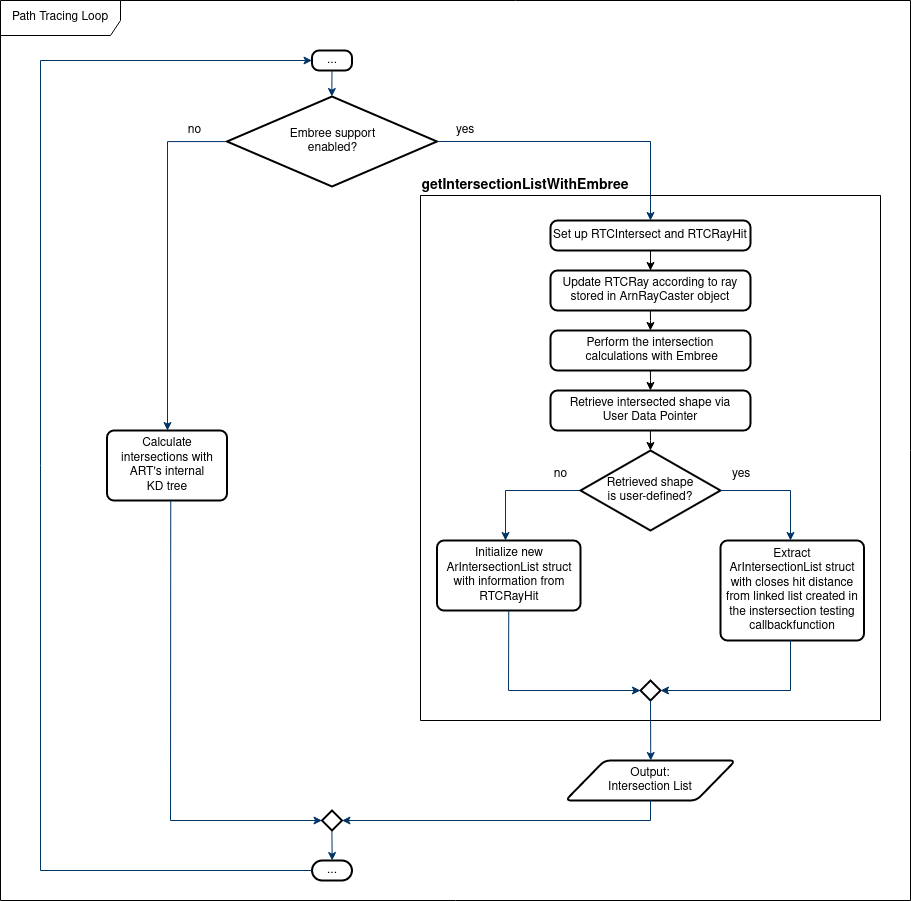
\includegraphics[width=1\linewidth]{img/3 approach/getIntersectionListWithEmbree.png}
	\caption{Flowchart the workflow of ray tracing with Embree in ART. The nodes with the three dots depict the internal procedures of ART.}
	\label{fig:raytracing_chart}
\end{figure}

In the body of this function, an \texttt{RTCIntersectContext} is set up and a \texttt{RTCRayHit} struct is declared and updated according to the state of the \texttt{ArnRayCaster} object: The information with which the \texttt{RTCRayHit} stuct is being updated contains the orientation and direction of the ray that is stored as an instance variable of the \texttt{ArnRayCaster} object, and the ID associated to the ray. The \texttt{tfar} value of is initialized with Objective-C's \texttt{INFINITY} macro and the \texttt{geomID} field of the \texttt{RTCHit} struct is initialized with the macro \texttt{RTC\_INVALID\_GEOMETRY\_ID}. 

Embree utilizes single-precision floating-point numbers for its internal calculations, whereas ART uses double-precision floating-point numbers. To compensate for visual artifacts in the final image, we do not initialize the \texttt{tnear} value of the \texttt{RTCRay} with zero. Instead, we give it a little offset to prevent calculating an intersection between a secondary ray and the same shape that was already hit. We found the value $1\cdot 10^{-3}$ to be reliable. A comparison of an image rendered with and without this offset is given by Figure \ref{fig:offset}.

\begin{figure}[!tbp]
	\centering
	\subfloat[Result of rendering a simple scene when the \texttt{tnear} value of the \texttt{RTCRay} is set to zero.]{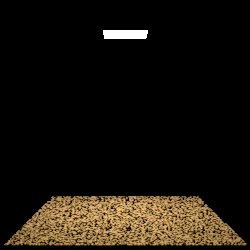
\includegraphics[width=.4\textwidth]{img/3 approach/artifact_2.png}}
	\hfil
	\subfloat[Result of rendering a simple scene when the \texttt{tnear} of the \texttt{RTCRay} is given an offset of $1\cdot 10^{-3}$.]{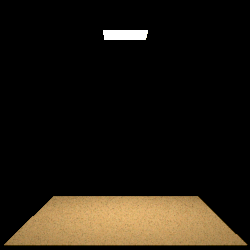
\includegraphics[width=.4\textwidth]{img/3 approach/artifact.png}}
	\caption{Artifact caused by the conversion of the hit distance of the ray from a double-precision floating-point number to a single-precision floating-point number. Due to an imprecise calculation of the intersection point, a secondary ray might intersect the same shape again.}
	\label{fig:offset}
\end{figure}

After the update of the \texttt{RTCRayHit} struct, the actual ray tracing is performed by the invocation of the \texttt{rtcIntersect1} function. Depending on whether a bounding box of a user-defined geometry or non-user-defined geometry in Embree's internal BVH was intersected by the \texttt{RTCRay}, either our custom callback function \texttt{embree\_intersect\_geometry} is called by Embree, or Embree performs the intersection testing with its built-in functionality.

Once the overall rendering job successfully completed, a "clean-up" is performed. The \texttt{GeometryData} structs associated with the scene are released, followed by the release of the \texttt{RTCScene} via the function \texttt{rtcReleaseScene} and the release of the \texttt{RTCDevice} via \texttt{rtcReleaseDevice}. As a final step, the \texttt{ArnEmbree} object \texttt{embreeManager} itself is released.


\subsection{Intersecting user-defined geometry}
\label{subsec:instersect}

In case a bounding box of a user-defined geometry is intersected with an \texttt{RTCRay}, the callback function \texttt{embree\_intersect\_geometry} is invoked by Embree. In this function, the \texttt{Geometry Data} struct associated with the geometry in question is retrieved via the geometry user data pointer. 

\begin{figure} 
	\centering
	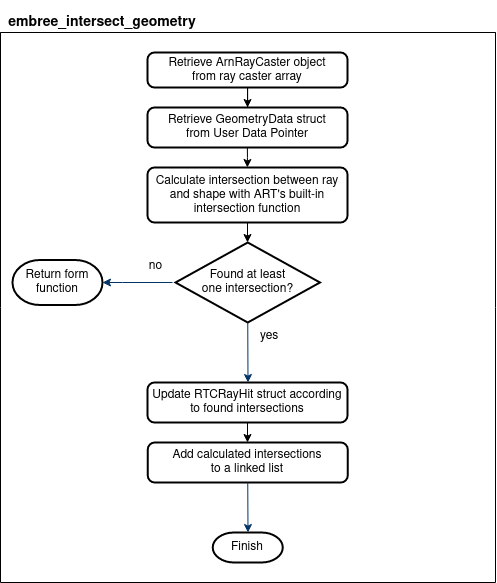
\includegraphics[width=.8\linewidth]{img/3 approach/inetsect_flowchart.png}
	\caption{Workflow of the custom \texttt{embree\_intersect\_geometry} callback function.}
	\label{fig:intersecting_chart}
\end{figure}

Subsequently, an empty \texttt{ArIntersectionList} struct is declared and the intersection between ART's representation of the ray and the shape is calculated via calling the \texttt{getIntersectionList} function of the \texttt{Combined Attributes} object, which takes a reference to the empty \texttt{ArIntersectionList}, as well a reference to the \texttt{ArnRayCaster} object as input.
This function will calculate the intersection points on the shape and update the \texttt{ArIntersectionList} struct accordingly. The reason why the \texttt{getIntersectionList} instance method of the \texttt{Combined Attributes} object is called, rather than the \texttt{getIntersectionList} instance method of the shape object, is that by doing so, the transformation information of the shape will be taken into account.

If no intersection was found, we return immediately from the \texttt{embree\_intersect\_geometry} function. Otherwise, we will update the \texttt{tfar} value of the \texttt{RTCRay} with the hit distance and the geometry ID of the \texttt{RTCHit} struct with the geometry ID associated with the intersected shape.
The resulting \texttt{ArIntersectionList} is then stored in a linked list.

After the invocation of the \texttt{rtcIntersect1} function in the body of the  \texttt{getIntersectionListWithEmbree} function, the geometry ID of the \texttt{RTCHit} is evaluated. If the value of this variable remains \texttt{RTC\_INVALID\_GEOMETRY\_ID}, we conclude that no intersection was found and we return an empty \texttt{ArIntersectionList}. Otherwise, we retrieve the \texttt{RTCGeometry} that has been intersected with the geometry ID.

This \texttt{RTCGeometry} is used for the retrieval of the associated \texttt{GeometryData} struct via the user data pointer. Based on the Boolean variable \texttt{\_isUserGeometry}, we check whether the intersected shape is a user-defined geometry or a simple indexed geometry.

For the latter, we initialize the empty \texttt{ArIntersectionList}, that was passed to the \texttt{getIntersectionListWithEmbree} function "from scratch" with the updated \texttt{tfar} value of the \texttt{RTCRay}, the shape object of the \texttt{GeometryData} struct, and the \texttt{ArnRayCaster} object itself. This newly initialized \texttt{ArIntersectionList} is then returned from the \texttt{getIntersectionListWithEmbree}.

In case the intersected geometry is a user-defined geometry, the linked list, in which the calculated \texttt{ArIntersectionList}s where placed during the intersection testing, must contain at least one \texttt{ArIntersectionList} struct. We locate the \texttt{ArIntersectionList}, whose head has the minimal hit distance, by linear search. When this \texttt{ArIntersectionList} is located, we extract it from the linked list and release all other \texttt{ArIntersectionList}s stored in it. The extracted list is then assigned to the initially empty \texttt{ArIntersectionList} that was passed to the \texttt{getIntersectionListWithEmbree} function, and ART proceeds as usual until the next ray is cast.


\subsection{Resolving of encountered issues}
\label{sec:issues_user}
The following subsection outlines two major issues encountered with the approach described in the last sections. We furthermore describe how these issues can be resolved.

\subsubsection{Multi-threaded intersection testing for user-defined geometry}
As briefly mentioned in Chapter \ref{chap:art}, ART supports ray tracing with multiple threads.
Before the ray tracing procedure is initiated by ART, copies of the \texttt{ArnRayCaster} object are created for each thread. A copy of the scene graph and the KD tree is assigned to each copy of the \texttt{ArnRayCaster} object to ensure lock-free parallelism.

However, the implementation of the \texttt{embree\_intersect\_geometry} callback function for intersecting user-defined geometry is not thread safe. This is due to the \texttt{ArnRayCaster} object that needs to be passed as an argument to the \texttt{getIntersectionList} function of the \texttt{Combined Attributes} object inside the \texttt{embree\_intersect\_geometry} function.

For a simple retrieval of the \texttt{ArnRayCaster} inside our custom intersection callback function, a static reference to it was originally initialized. This works fine when performing rendering jobs with only a single thread. If multiple threads are involved in the intersection computations, the procedure outlined in Subsection \ref{subsec:instersect} is prone to errors since multiple \texttt{ArnRayCaster} objects are traversing and altering a single copy of the scene graph.

To archive lock-free parallelism, we need to retrieve the "right" \texttt{ArnRayCaster} copy associated with the current thread in the interior of the intersection callback function. However, we cannot utilize the user data pointer for this since the user data pointer is associated with the scene geometry, which can be intersected by multiple rays belonging to different \texttt{ArnRayCaster} objects on different threads at the same time.

For the placement of an \texttt{ArnRayCaster} into and for the retrieval of an \texttt{ArnRayCaster} from the ray caster array, we use an identifier of the thread associated with it. We obtain the thread ID via invocation of the \texttt{gettid} function, provided with the \texttt{unistd} header file, for accessing the POSIX operating system API. The reason we chose the function \texttt{gettid} over the function \texttt{pthread\_self}, is that for $n$ cores involved for rendering, \texttt{gettid}, called from $n$ different threads, will return $n$ strictly consecutive integer values. With the help of these values we can write a fairly simple "hash" function for placing \texttt{ArnRayCaster} pointers in the ray caster array and for retrieving them from it in our intersection callback function: The index of the particualar \texttt{ArnRayCaster} pointer will be the thread ID received by the \texttt{gettid} function taken modulo with the counter variable.

During the beginning of the ray tracing procedure, a reference to the  \texttt{ArnRayCaster} object associated with the current thread is added to the ray caster array, if not already been done, retrieved in the interior of the intersection callback function in constant time, and passed to the \texttt{getIntersectionList} function of the \texttt{Combined Attributes} object. 

The head of the linked list, in which the collected intersection lists are stored, is made an instance variable of the \texttt{ArnRayCaster} class, which allows for a simple retrieval of these intersection lists outside the intersect callback function. 

\subsubsection{Intersecting infinite spheres}

A specific type of geometry supported by ART is a sphere with a huge radius. These \emph{infinite spheres} are used in a virtual scene for environment lighting.
Due to its radius, the length of the bounding box edges enclosing the infinite sphere is twice the infinite sphere's radius. 
Generally speaking, axis-aligned bounding boxes can be described by two vertices in Euclidean space, connected via the bounding box's body diagonal. In this subsection, we will refer to these vertices as \emph{upper point} and \emph{lower point}. 

In ART, all three coordinates of the upper point are set to a huge value, represented by the double value \texttt{MATH\_HUGE\_DOUBLE}, and respectively, all three coordinates of the lower point are set to the negative of that value, \texttt{- MATH\_HUGE\_DOUBLE}.

\begin{listing} 
	\begin{lstlisting}[caption={Casting of a double precision floating point number to a single precision floating point number by explicit conversion.}, label={lst:casting}]
	struct RTCBounds * bounds_o = args->bounds_o;
	
	bounds_o->lower_x = (float) boundingBox.min.c.x[0];
	bounds_o->lower_y = (float) boundingBox.min.c.x[1];
	bounds_o->lower_z = (float) boundingBox.min.c.x[2];
	
	// ...
	\end{lstlisting}
\end{listing}

As mentioned in Subsection \ref{sec:embree_raytracing}, Embree uses single-precision floating-point numbers for its internal calculations. ART, on the other hand, uses double-precision floating-point numbers. Therefore, after calculating the double values describing the bounding box, we cast them to float values via the explicit conversion operator in \texttt{C/C++} before passing them to Embree, as shown in Listing \ref{lst:casting}.  
When, during ray tracing, the \texttt{tfar} value of the \texttt{RTCRay} is set to the single-precision representation of infinity by Objective-C, the bounding box is never intersected. This is due to intersection testing being only performed in the interval $[1\cdot 10^{-3},\infty]$ and Objective-C's representation of infinity is "smaller" than the value \texttt{MATH\_HUGE\_DOUBLE}. The bounding box enclosing the infinite sphere is never intersected by an \texttt{RTCRay}.

Fortunately, ART provides a representation for infinity as a single-precision number as well, \texttt{MATH\_HUGE\_FLOAT}. Therefore, we can resolve this issue by checking in the \texttt{embree\_bbox} callback function whether the two vertices of the calculated bounding box have the coordinates \texttt{MATH\_HUGE\_DOUBLE} (and resp. \texttt{-MATH\_HUGE\_DOUBLE}) and updating them with the value \texttt{MATH\_HUGE\_FLOAT} (and resp. \texttt{-MATH\_HUGE\_FLOAT}). By doing so, Embree can detect intersections between an \texttt{RTCRay} and the bounding box of the infinite sphere, and the intersection with the sphere itself can be calculated.

However, we decided to exclude Embree functionality from intersection testing with this type of shape. The reason for this lies in the further reduction of the number of unnecessary intersection calculations. If an intersection point on the infinite sphere is occluded by other scene geometry, we can ignore it. Therefore we only calculate the intersection between a ray and the infinite sphere if the ray did not intersect other scene geometry.

\subsubsection{Consecutive intersection of user-defined and non-user-defined geometry}

With the approach described in Section \ref{subsec:instersect}, an issue arises when ray tracing virtual scenes which contain both user-defined and non-user-defined geometry. In such scenes, a cast ray could consecutively intersect a non-user-defined geometry and a user-defined geometry. To give an example, this is the case for the virtual scene displayed in \ref{fig:no_bunny}. This scene is composed of a quadrangle serving as the ground plane, the Stanford Bunny triangle mesh, which was provided by the Stanford 3D Scanning Repository \cite{plyRepo}, and an infinite sphere for environment lighting.

Given a ray that first intersects the PLY mesh and subsequently the infinite sphere, we noticed that through the invocation of the \texttt{rtcIntersect1} function, Embree internally calculates the intersections between the ray and the triangle mesh first and then calls the \texttt{embree\_intersect} callback function to calculate the intersection point with the infinite sphere.


\begin{figure}[!tbp]
	\centering
	\subfloat[Scene rendered with Native ART.]{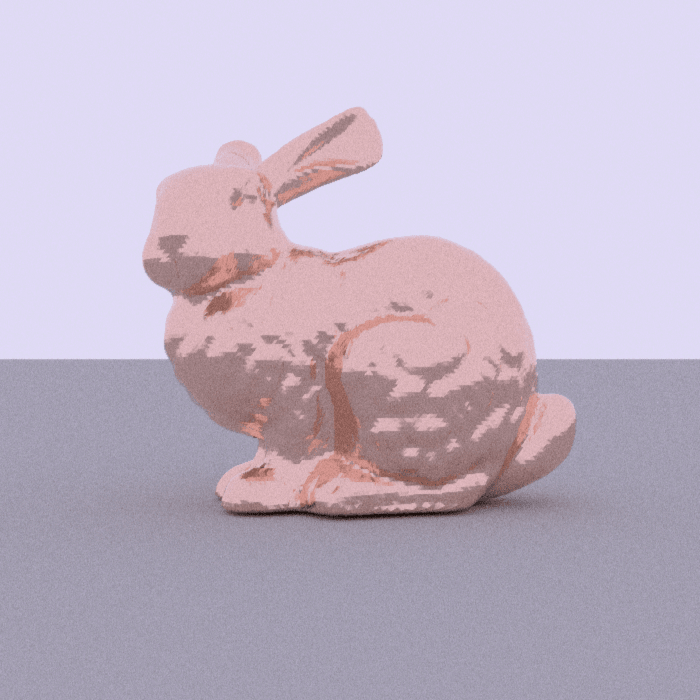
\includegraphics[width=.4\textwidth]{img/3 approach/bunnyNormal.png}} 
	\hfil
	\subfloat[Scene rendered with the approach outlined in Section \ref{sec:embree_raycasting}]{
\includegraphics[width=.4\textwidth]{img/3 approach/bunnyError.png} \label{fig:no_bunny_close}}
	\caption{Rendered images of a scene containing a non-user-defined triangle mesh and quadrangle, and a user-defined user-defined infinite sphere, illuminating the rest of the sphere.}
	\label{fig:no_bunny}
\end{figure}


The problem, which arises here, is that the values of the \texttt{RTCRayHit} struct, e.g., the \texttt{tfar} value of the \texttt{RTCRay}, are updated with information corresponding to the intersection with the triangle mesh first. Afterward, the user-defined infinite sphere is intersected, and the intersection calculation is performed by our custom \texttt{embree\_intersect\_geometry} function. In this function, we overwrite the values of the \texttt{RTCRayHit} struct that has been previously calculated while the triangle mesh was intersected. Therefore, the information regarding the intersections between the \texttt{RTCRay} and the triangle mesh is lost, and only the \texttt{ArIntersectionList} storing the intersections with the infinite sphere is present in the linked list. A result of this behavior can be seen in Figure \ref{fig:no_bunny_close}.

To resolve this issue, we make use of a slight modification: In the \todo{use algorithm} \texttt{embree\_intersect\_geometry} callback function, before performing the actual intersection calculation between a ray and a user-defined geometry, we check whether the value of the geometry ID of the \texttt{RTCHit} struct remains being set to \texttt{RTC\_INVALID\_GEOMETRY\_ID}. If this is not the case, and if the head of the linked list storing the collected intersections is not \texttt{NULL}, we conclude that an intersection with a non-user-defined geometry must have already been calculated. We assume that is intersection already contains the closest distance to the ray origin. With the help of the geometry ID, we retrieve the associated \texttt{GeometryData} struct for the geometry in question from the linked list storing all the \texttt{GeometryData} structs linked to the scene geometry. With the information stored in this \texttt{GeometryData} struct, we initialize a \texttt{ArIntersectionList} "from scratch" and add it to the linked list storing the collected intersections.

With this approach, all the scenes on which our implementation was tested (which will be introduced in Chapter \ref{chap:results}) could be rendered without further problems.


\section{Rendering CSG with Embree}
\label{sec:embree_csg}

Unfortunately, Embree does not support rendering of constructive solid geometry direct. However, this does not mean that ray tracing CSG with Embree is completely impossible. The following section outlines three different approaches for ray tracing virtual scenes containing constructive solid geometry in ART with the help of Embree.

Since Embree is an open-source framework, one could consider rigging Embree itself for suitable CSG rendering. Nevertheless, we refrained from such an undertaking because of two reasons: On one hand, it is possible that the altering of the Embree framework would exceed the scope of this thesis. On the other hand, we want our integration to be compatible with the original Embree framework in its current and future versions.

We, therefore, consider Embree as a "black box" for which we provide information such as a ray origin and direction and receive in turn information concerning intersections with the scene geometry such as the hit distance and the surface normal at the hit point.


\subsection{Evaluation of collected intersections according to the scene graph}
\label{subsec:apprach1}

In the past, an attempt for the implementation of CSG rendering with Embree was conducted by Markéta Karaffová and described in her master thesis \cite{karaffova2016}. Her approach consists of the collection of intersections between the scene geometry and a ray that Embree calculates and their subsequent evaluation according to a provided CSG tree as described in Subsection \ref{subsec:csg_into}.
With the approach outlined in this subsection, we adapt the approach described in \cite{karaffova2016} for ART. We were not intimidated by the increased rendering times that result from the implementation described in \cite{karaffova2016} since we believed we would be able to improve it for ART.

For our approach outlined in this subsection, we will only consider CSG that are composed of user-defined geometry.

The intersections between a ray and user-defined scene geometry can be collected via storing the corresponding \texttt{ArIntersectionLists} in a linked list as described in subsection \ref{subsec:instersect}. One advantage of maintaining such a "list of intersection lists" as opposed to the merging the individual \texttt{ArIntersectionList}s into a single larger \texttt{ArIntersectionList}, is having the \texttt{ArIntersectionList} separated according to the shape associated with them. This is convenient since ART provides functions for evaluating two given \texttt{ArIntersectionList} structs according to the binary operators \texttt{OR}, \texttt{AND} and \texttt{SUB} as described in Subsection \ref{subsec:csg_into}. To avoid confusion, we will refer to the \texttt{ArIntersectionList} struct as \emph{intersection list} and to the linked list, which stores individual \texttt{ArIntersectionList} structs as \emph{intersection linked list}.

The ray tracing of the geometric primitives proceeds as outlined in Subsection \ref{subsec:instersect}
Once the intersection calculation with Embree has finished, we retrieve the associated \texttt{GeometryData} struct of the intersected geometry. We then evaluate the collected intersections stored in the intersection linked list according to the original scene graph.

During the evaluation, the subgraph rooted at the Bounding Box node that is a direct child of the BSP Tree node (compare Figure \ref{fig:scene_graph}) is traversed until the leaves representing the shape are reached. Due to the reason that intersections between the ray and some shapes have already been calculated previously by Embree, we first check whether an intersection list associated with the shape in question is already present in the intersection linked list. If this is the case, the corresponding intersection list is located in the intersection linked list by linear search, extracted from it, later evaluated according to the CSG tree, which is, in our case, the original scene graph.

Since ART supports instancing of geometry, meaning that multiple instances of the shape with different associated Combined Attributes nodes exist in the scene, we use the Combined Attributes node as a unique identifier to retrieve the right intersection list from the intersection linked list.
Therefore, we add a reference to the \texttt{Combined Attributes} object of a shape to the \texttt{ArIntersectionList}. This \texttt{Combined Attributes} object is associated with the shape whose intersections with a ray are stored in the \texttt{ArIntersectionList} struct.


After the evaluation, the intersection list, whose head intersection has the minimal distance to the ray origin, is extracted from the intersection linked list, and the ray tracing procedure precedes as usual.

\subsubsection{Limitations of this approach}

Although it is possible to render CSG with the approach outlined in this subsection, we are aware that it is still far from being optimal. We have not implemented this functionality for non-user-defined geometry. When Embree calculates the intersections between a ray and a non-user-defined geometry, it returns only one intersection, either the closest or an arbitrary one \footnote{However, \cite{karaffova2016} describes a method of how all encountered intersections can be retrieved from Embree.}.

The whole original scene graph is traversed to evaluate the intersections between a ray and a CSG represented by only a subgraph. Theoretically, only this subgraph would need traversing. However, even those subgraphs representing a particular CSG in the scene graph can be large and complex. To give an example, Figure \ref{fig:rotonda_intro} shows a rendered image of the "Villa Rotonda". The entire villa comprises only two CSG, which are constructed from a total number of 1,255 primitives.

\begin{figure}
	\centering
	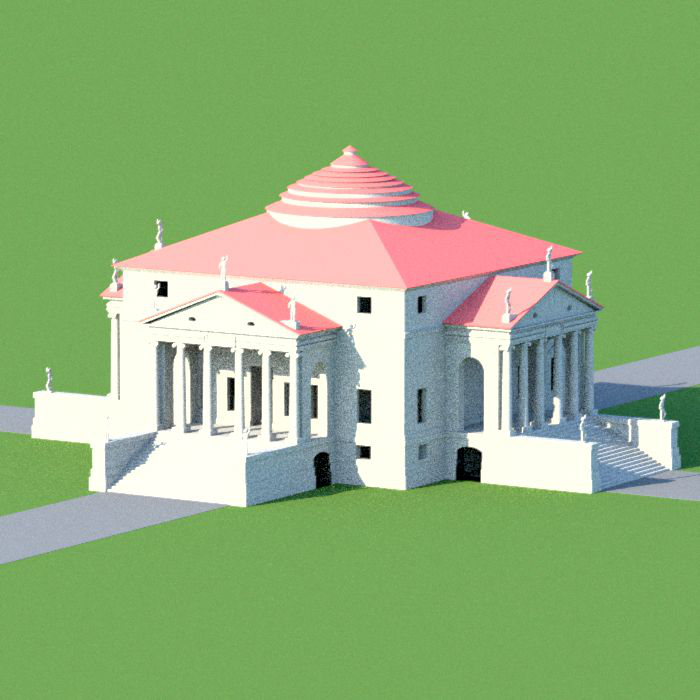
\includegraphics[width=.5\linewidth]{img/3 approach/villaRotondaNormal.png}
	\caption{Rendered image of the Villa Rotonda model.}
	\label{fig:rotonda_intro}
\end{figure}

Even evaluating the found intersections according to the subgraph associated with only one of the two CSG would be time-consuming. We realized the following: Even if we worked on optimizing the procedure outlined in this subsection, the lead we gained through Embree over Native ART would be compensated for by the subsequent scene graph traversal. It even could be that the performance of the overall ray tracing procedure of ART would be decreased for complex scenes, such as the Villa Rotonda scene in Figure \ref{fig:rotonda_intro}.

Since the motivation behind the goal of this thesis, namely the integration of Embree into the CSG rendering framework ART, was the acceleration of ART's ray tracing procedure, we decided that further optimizations of this approach would not be profitable.


\subsection{Initializing the complete CSG as user-defined geometry}
\label{subsec:apprach2}

The increased render times that resulted from the previous approach served as a motivation for developing different procedures for ray tracing CSG with Embree. We want to avoid a subsequent scene graph traversal and at the same time still treat Embree as a black box.

The idea of the approach described in this subsection lies in the initialization of the whole constructive solid geometry as a user-defined geometry instead of the geometric primitives it is composed of. The bounding box for such a CSG will be calculated with a function provided by ART and passed to Embree.
If this bounding box would be stored in Embree's internal BVHs, intersected by an \texttt{RTCRay} during the ray casting procedure, ART's internal structures would be used for the continuative traversal to calculate the intersections with the geometric primitives. This undertaking seems like a satisfactory compromise between ART and Embree.
 
For our new approach, we define the \emph{topmost CSG node} in the scene graph as the root node of the subgraph that represents the CSG. The geometric primitives represented by the leaf nodes of this subgraph are the geometric primitives of which the CSG is composed. For example, when considering the scene graph, assembled by ART to render the scene shown in Figure \ref{fig:csg_or}, which itself is shown in Figure \ref{fig:scene_graph}, the topmost CSG node of the CSG is the "\texttt{OR}-node". The single leaf of the subgraph rooted at that node is the shape node that represents a sphere object.

When during the initial assembly of ART's internal scene graph such a topmost CSG node is encountered, a class method of the \texttt{ArnEmbree} class, \texttt{initEmbreeCSGGeometry}, is called, which initializes  a CSG as a user-defined geometry for Embree according to procedures explained in Subsection \ref{sec:init_user}. 


\begin{listing} 
	\begin{lstlisting}[caption={Updated \texttt{GeometryData} struct for CSG rendering.}, label={lst:geometry_data_final}]
	// each geometry in the scene is associated with
	// this stuct, it is needed for embree to
	// perform user defined geometry intersection
	// calculations
	typedef struct GeometryData 
	{
		unsigned int _embreeGeomID; // geometry id of the shape
		ArNode * _shape; // ART's shape representation in memory
		ArTraversalState _traversalState; // state of the RayCaster
		
		ArNode<ArpRayCasting> * _combinedAttributes_or_csg_node; // node used for ray casting
		BOOL _isUserGeometry; // determines if geometry is user-defined or non-user-defined
	}
	GeometryData;
	\end{lstlisting}
\end{listing}

\texttt{GeometryData} structs are created for CSG, too. The struct itself was slightly adapted for CSG rendering. As can be seen in Listing \ref{lst:geometry_data_final}, we renamed the variable storing a reference to the \texttt{Combined Attribute} node to \texttt{\_combinedAttributes\_or\_csg\_node}. Both the Combined Attributes node object and the topmost CSG node derive from the \texttt{ArNode} base class, and through the implementation of the \texttt{ArpRayCasting} protocol, they provide functionality for calculating bounding boxes and performing intersection testing.
When a CSG is getting initialized as a user-defined geometry, a reference to the topmost CSG node is assigned to the
\texttt{\_combinedAttributes\_or\_csg\_node} variable instead of a reference to the \texttt{Combined Attributes} object.

A flag gets activated after a successful initialization of a CSG for Embree during the scene graph assembly. When the traversal of the scene graph continues to the leaf nodes representing the geometric primitives of the CSG, they do not get initialized as user-defined geometry if this flag is activated.

During the intersection calculation by the \texttt{embree\_intersect} callback function, the \texttt{getIntersectionList} function associated with the \texttt{\_combinedAttributes\_or\_csg\_node} object is called. Depending on this node being a \texttt{Combined Attributes} node or a topmost CSG node, the rendering procedure diverges: For a \texttt{Combined Attributes} node, the intersections are calculated directly on the shape, taking transformation information into account. For a topmost CSG node, the intersections with the underlying primitives are calculated by traversing the sub scene graph rooted at that node, as outlined in Section \ref{sec:art_raytracing}, only with the difference that with this approach, only a subgraph of the original scene graph is traversed.

During the scene graph assembly for scenes with environment lighting, ART connects the infinite sphere with the rest of the geometries in the scene with a union operator. This is undesirable since our implementation would treat the entire geometries contained in the scene as one CSG. We can compensate for this by checking if a given topmost CSG node that is about to be initialized for Embree has an infinite sphere as a direct child. If so, we are not initializing this topmost CSG node for Embree.

With this approach, scenes containing constructive solid geometries can be successfully rendered, and the performance of the ray tracing process increased noticeably compared to the previous approach. Furthermore, the artifacts that result from rendering a scene ART by traversing of the original scene graph, as described in Subsection \ref{sec:art_raytracing}, such as the visible noise, are not present in images rendered with this approach. We cannot give a definite answer on why these artifacts are disappearing when rendering scenes with this approach. However, we believe this resolution must be related to the only partial traversal of the original scene graph.

\subsubsection{Limitations of this approach}

An inconvenience of this approach is that the fact that Embree treats the entire CSG as a single geometry must be taken into account by a user when modeling a scene for ART. For example, Figure \ref{fig:cb} shows rendered images of the Cornell Box. For rendering the scene with Native ART, one could apply a union operator to the geometry of the box itself and the geometry describing the area light source (which is depicted as a box itself). Our approach, however, would interpret these two geometries as a single CSG and traverse the original scene graph to find intersections between them and a given ray. It would be better to describe the box of the Cornell Box and the area light as two disjoint geometrical entities.


An issue was encountered when rendering a specific CSG scene: The Villa Rotonda scene, shown in Figure \ref{fig:rotonda_intro}. Figure \ref{fig:rotonda_embree} shows the final image, rendered by the described approach. The figure shows the villa with its roof missing (compare Figure \ref{fig:rotonda_intro}). We have to admit that we were not able to resolve this issue yet. However, rendering the scene with Native ART by traversal of the original scene graph results in the same artifact (besides the visible noise). Due to this and the fact that we did not encounter this issue with other scene files containing CSG (compare Chapter \ref{chap:results}), we assume that this is the issue is due to a bug occurring during the scene graph assembly for this scene in ART.

\begin{figure}
	\centering
	\subfloat[Villa Rotonda scene rendered with the implementation outlined in this subsection.]{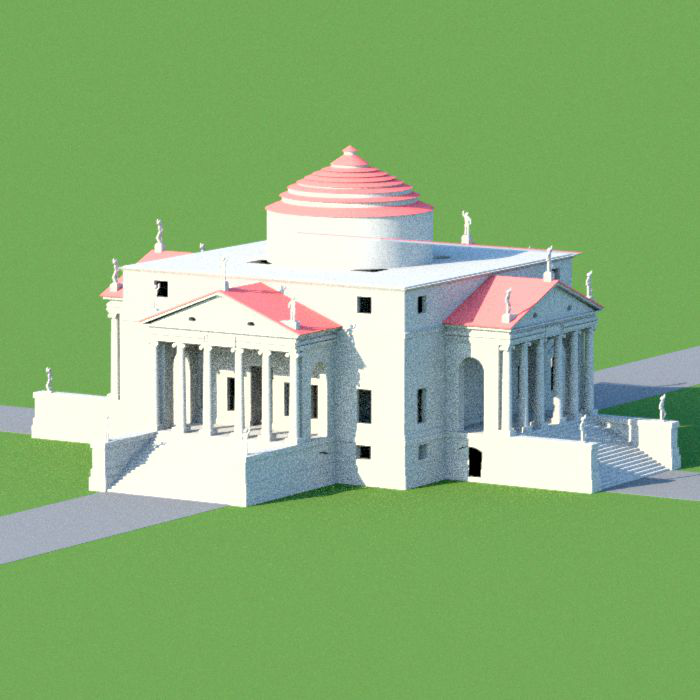
\includegraphics[width=.4\textwidth]{img/3 approach/villaRotondaEmbree.png}\label{fig:rotonda_embree}}
	\hfil
	\subfloat[Villa Rotonda scene rendered with Native ART by traversing the original scene graph.]{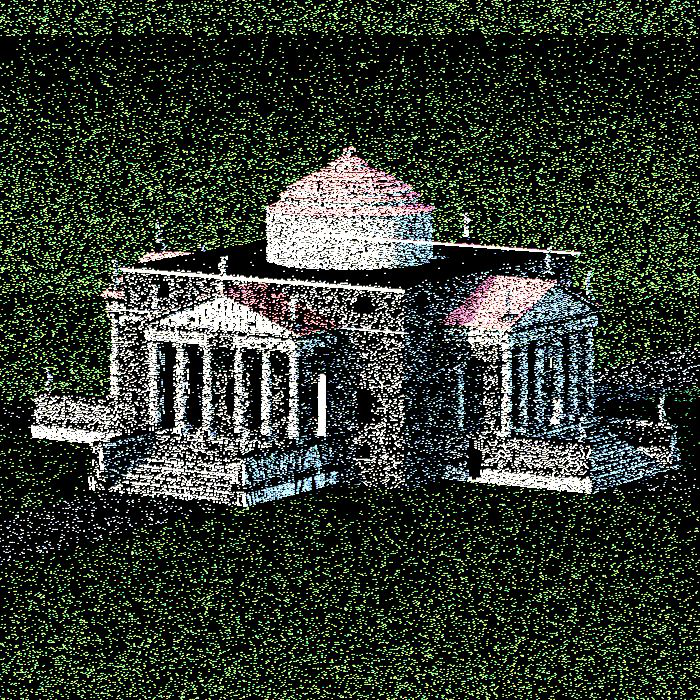
\includegraphics[width=.4\textwidth]{img/3 approach/villaRotondaOrgScenegraph.png}\label{fig:rotonda_orgscenegraph}}
	\caption{Artifact in the Villa Rotonda scene: The villa is missing its roof.}
	\label{fig:rotonda}
\end{figure}


\begin{figure}
	\centering
	\subfloat[Scene rendered with native ART by traversing the internal KD tree.]{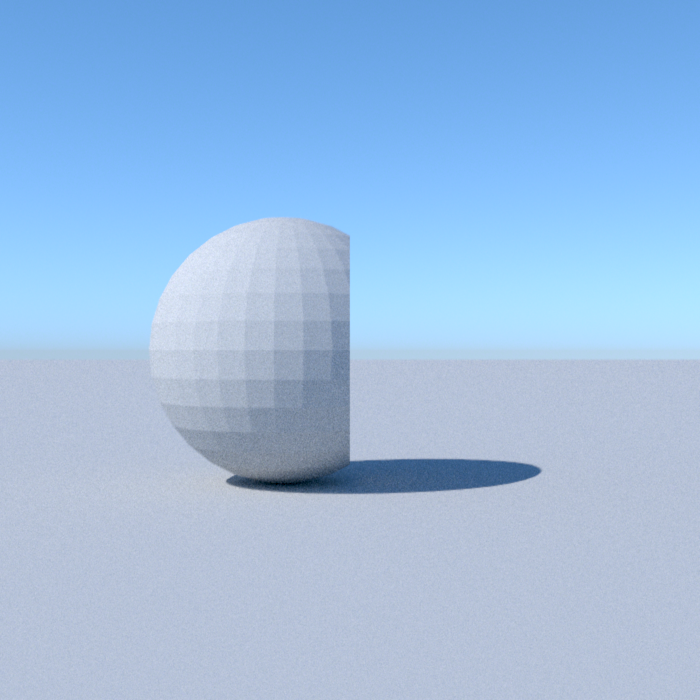
\includegraphics[width=.4\textwidth]{img/3 approach/spheresEmbree.png}\label{fig:csg_mesh_intro_normal}}
	\hfil
	\subfloat[Artifact in the scene rendered with the approach outlined in this section.]{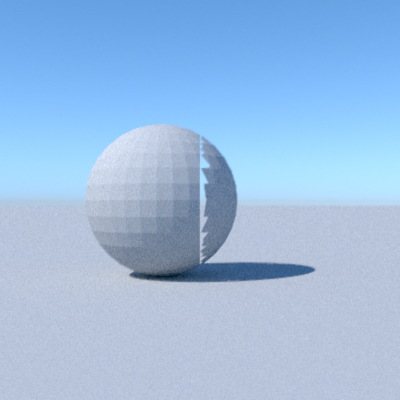
\includegraphics[width=.4\textwidth]{img/3 approach/EmbreeOrgScenegraph.png}\label{fig:csg_mesh_intro_embree}}
	\caption{CSG composed of triangle meshes. The figures show a scene with two spheres described as triangle meshes. The right sphere is "subtracted" from the left sphere via the Boolean set operation \texttt{OR}. The scene can be regarded as the counterpart of the scene shown in Figure \ref{fig:csg_sub} for triangle mesh primitives.}
	\label{fig:csg_mesh_intro}
\end{figure}

Furthermore, the rendering of CSG that is composed of at least one triangle mesh leads to artifacts. As mentioned, triangle meshes are associated in ART with individual KD trees that accelerate the intersection calculations solely between a ray the particular triangle mesh. When we initialize a triangle mesh for Embree, we omit the construction of individual mesh KD trees because they are not needed when ray tracing triangle meshes in general. However, when treating a CSG constructed from triangle meshes as a user-defined geometry and thus using ART's internal structures to calculate the intersections with the primitives, we depend on these individual KD trees for triangle meshes. Resurrecting these individual KD trees alone is not enough to resolve the artifact since the transmission from the original scene graph to the individual KD Tree at the Shape node representing the triangle mesh is not seamless.


\subsection{Creation of KD trees for CSG}
\label{subsec:apprach3}

The artifact shown in the rendered image of the Villa Rotonda scene, which is visible in Figure \ref{fig:rotonda_embree}, as well as the artifacts that arise when rendering CSG that is composed of triangle meshes, as shown in Figure \ref{fig:csg_mesh_intro}, motivated us to develop further our approach outlined in the previous section. The initial idea for resolving these artifacts was to build ART's internal KD tree over the entire scene and, when a bounding box of a CSG is intersected by Embree, to continue the traversal to the CSG primitives in the subtree of the KD tree describing the spatial area in which the CSG is located.
However, associating a Shape node in the scene graph to the area subdivided by the split planes of the KD trees, in which the shape is located, is not obvious since multiple geometries can be located in such an area.

The approach outlined in this subsection, which can be reagrded as an extension for the approach described in the previous subsection, was inspired by the individual KD trees for the triangle meshes and the work of Petr Zaji\v{c}ek, documented in his master thesis \cite{zajicek2012}. In this thesis, Zaji\v{c}ek describes the application of KD trees to scenes containing CSG.

For the scenes containing CSG, instead of constructing one KD tree that subdivides the bounding box of the entire scene, we construct multiple smaller KD trees for subdividing the bounding box of the CSG present in the scene.
Therefore, we add a Boolean variable to the \texttt{GeometryData} struct shown in Listing \ref{lst:geometry_data_final}, indicating whether the associated geometry is a CSG or not. Before committing the \texttt{RTCScene} that will trigger the construction of Embree's internal BVH, we iterate through the linked list storing all \texttt{GeometryData} structs that are associated with the scene geometry. With the help of the \texttt{GeometryData} struct, we check whether the associated geometry is a CSG. If so, we calculate the bounding box that encloses the CSG and construct a KD tree that further subdivides the bounding volume. To calculate the bounding box and the KD tree, we use functions provided by ART. Furthermore, we add a reference to the root of the constructed KD tree to the \texttt{GeometryData} associated with the CSG.

During ray tracing with Embree, we retrieve the \texttt{GeometryData} corresponding to the intersected shape and verify if that shape is a CSG or not. If not, the ray tracing procedure continues as outlined in Subsection \ref{subsec:instersect}. Otherwise, we traverse the associated KD tree beginning at the root node, calculating the intersections with the CSG primitives and storing the resulting intersection list in the intersection linked list.

By traversing the individual KD trees to calculate intersections with CSG primitives, the issue regarding the Villa Rotonda scene described in the previous section is resolved \footnote{Figure \ref{fig:csg_rotonda} shows the scene rendered with the additional KD trees}. Furthermore, we are able to render CSG that is composed of triangle meshes.

\subsubsection{Limitations of this approach}

A disadvantage of this approach is that it depends on the internal KD trees associated with triangle meshes by ART. Their construction was originally omitted when initializing triangle meshes for Embree. However, by constructing those mesh KD trees for this approach, the decrease of the time needed to prepare the scene for ray tracing is compensated.
\chapter{Results and discussion}
\label{chap:results}

Our approach to integrating Embree into ART, as outlined in the previous chapter, was tested on a variety of scene files. This chapter provides an overview and analysis of the performance of our implementation. It is divided into three subsections. Subsection \ref{sec:results_csg} discusses the execution time of ART when rendering scenes CSG. A comparison is drawn between our two approaches for realizing CSG operations with Embree, the initialization of an entire CSG as a user-defined geometry and the traversal through the original scene graph or a dedicated KD tree. We will exclude the provision of results concerning the rendering of CSG through the collection of intersection points and their subsequent evaluation, outlined in Subsection \ref{subsec:apprach1}. This exclusion is due to the immense rendering time resulting from this approach, making it impractical.

Furthermore, we decided to test our implementation on virtual scenes, not necessarily containing CSG, to analyze the overall performance of rendering non-user-defined and user-defined geometries. Section \ref{sec:result_normal} provides the results on various scenes rendered by an hybrid implementation combining the approaches outlined in Subsections \ref{subsec:apprach2} and \ref{subsec:apprach3}. 

Finally, our implementation was tested on scenes, each containing triangle meshes of increasing triangle sizes. The outcome of these experiments is provided and evaluated in Section \ref{sec:result_meshes}.

The following experiments were conducted on an Asus N551JX laptop, which exhibits a quad-core Intel Core i7–4720HQ processor with a frequency of 2.6 GHz and 8 GB of RAM. The images shown in this chapter were rendered in ART with Embree support at a resolution of 700x700, a path length of 20, and a sample size of 128. The image synthesis of these scenes was performed by using the eight available cores of the machine.

\section{Evaluation of our integration for scenes containing CSG}
\label{sec:results_csg}

We tested the functionality of our implementation concerning CSG rendering with Embree on six scenes, which were made publicly available by the developers of ART \footnote{Most of the scenes shown in this chapter can be found in the \texttt{Gallery} folder of the ART repository, which is submitted together with this thesis as an electronic attachment. Scenes or 3D models that are not taken from this folder will be cited.}. All the scenes mentioned in this section contain an infinite sphere, serving as a skydome for illuminating the other scene geometry. 
\\

\noindent For this evaluation, our implementation was tested on the following scenes:
\begin{itemize}
	\setlength\itemsep{0.05em}
	
	\item The scene shown in Figure \ref{fig:csg_shell} consists of a single CSG, a procedurally modeled shell, and multiple cubes aligned to form a checkerboard pattern. The CSG, namely the shell, is composed of a total amount of 2,144 sphere primitives. The shell is modeled by arranging the spheres in spiral form and decreasing order according to their sizes. The largest sphere at the beginning of this sequence of spheres is "subtracted" by the \texttt{SUB} operator from the rest of the spheres. Then, the next largest sphere is "unified" by the \texttt{OR} operator with its preceding sphere in the sequence. This procedure is repeated for the remaining spheres in the sequence.
	
	\item  Figure \ref{fig:csg_orennayar} shows the rendered image of a scene composed of a cylinder serving as the ground on which three so-called \emph{grooved spheres} are placed. The grooves on the sphere result from applying a \texttt{SUB} operator to a group of six tori and the sphere in question.
	The purpose of this scene is to showcase ART's implementation of the Oren–Nayar reflectance model \cite{oren1994generalization} with different roughness grades.
	
	\item We have already encountered the \textbf{Villa Rotonda} scene in Subsection \ref{subsec:apprach1}. As mentioned there, the model of the Villa Rotonda is composed of two CSG with a total number of 1,255 primitives.
		
	\item The scene displayed in Figure \ref{fig:csg_torrancesparrow} is composed of twelve grooved spheres that are placed on three deformed cubes with different heights that together form a staircase. Furthermore, a cylinder serves as the ground. The initial purpose of this particular scene was the demonstration of the implementation of the Torrance–Sparrow reflectance model \cite{torrance1967theory} with varying roughness grades.
	
	\item Figure \ref{fig:csg_plane} shows a rendered image of a scene composed of a cylinder acting as the ground, and a biplane, composed of multiple CSG. The total number of topmost CSG nodes in the scene graph assembled by ART for this particular scene amounts to 28. The total number of geometric primitives of the 28 CSG is 336.
	
	\item Lastly, the rendered scene shown in Figure \ref{fig:csg_locomotive} shows a model of an Austrian steam locomotive. The single model is composed of multiple CSG, a total amount of 354 topmost CSG nodes are present in the scene graph associated with this scene The amount of geometric primitives present in the scene is 3,594.
	
	
\end{itemize}

\begin{figure}
	\centering
	\subfloat[Shell]{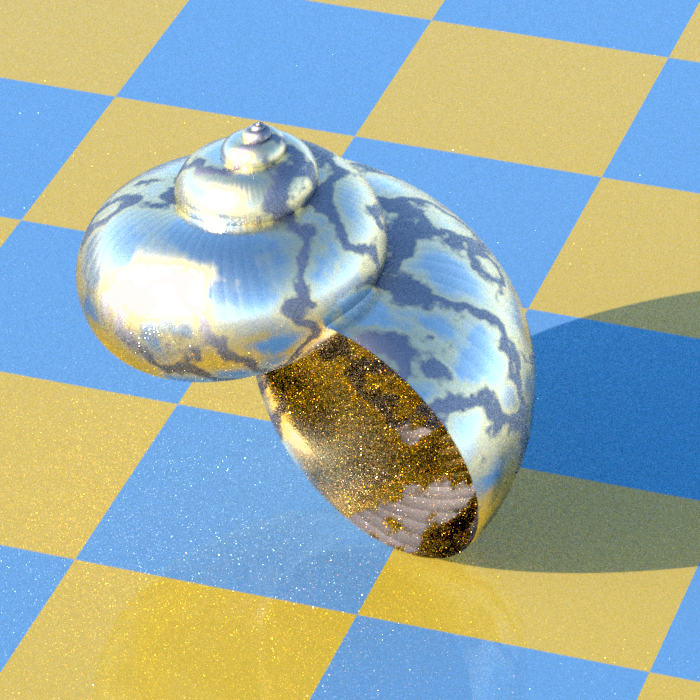
\includegraphics[width=.3\textwidth]{img/4 results/csg/snailEmbree.png}\label{fig:csg_shell}}
	\hfill
	\subfloat[Oren-Nayar Sphreres]{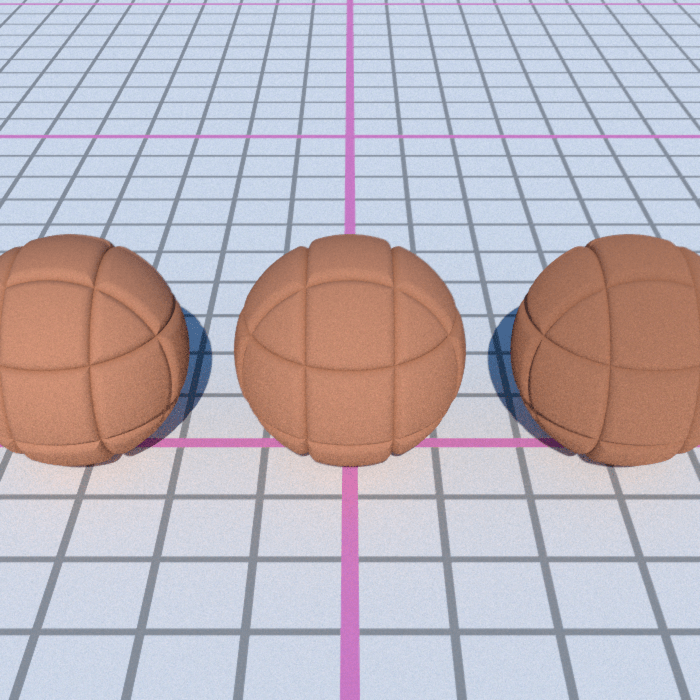
\includegraphics[width=.3\textwidth]{img/4 results/csg/orennayarEmbree.png}\label{fig:csg_orennayar}}
	\hfill
	\subfloat[Villa Rotonda]{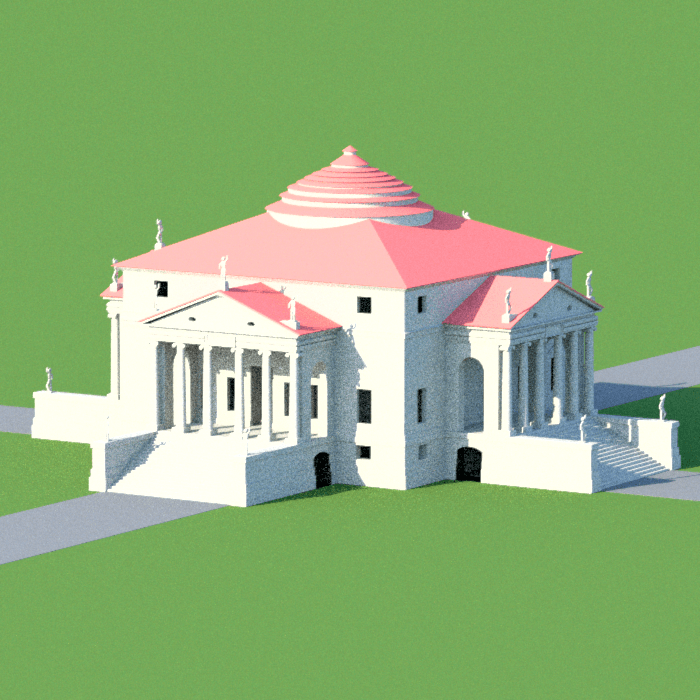
\includegraphics[width=.3\textwidth]{img/4 results/csg/rotondaEmbree.png}\label{fig:csg_rotonda}}
	\\
	\subfloat[Torrance-Sparrow Spheres]{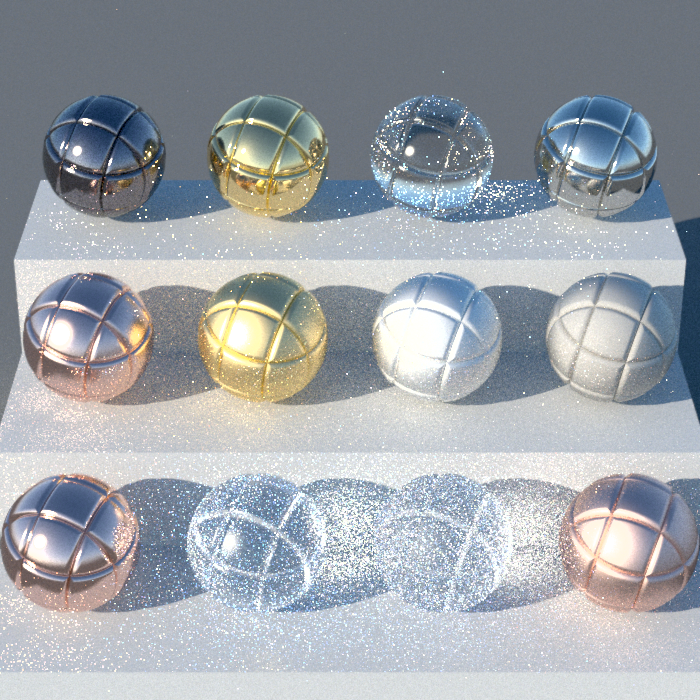
\includegraphics[width=.3\textwidth]{img/4 results/csg/torrancesparrowEmbree.png}\label{fig:csg_torrancesparrow}}
	\hfill
	\subfloat[Parked Biplane]{\includegraphics[width=.3\textwidth]{img/4 results/csg/planeEmbree.png}\label{fig:csg_plane}}
	\hfill
	\subfloat[Locomotive]{\includegraphics[width=.3\textwidth]{img/4 results/csg/locomotiveEmbree.png}\label{fig:csg_locomotive}}
	
	\caption{Scenes containing CSG, rendered with our implementation. The image of the Villa Rotonda shown in Figure \ref{fig:csg_rotonda} was rendered by traversing KD trees associated with the CSG in this scene. Unfortunately, the issue described in Subsection \ref{subsec:apprach2} remains when rendering the scene by traversing the original scene graph.}
	\label{fig:csg_figures}
\end{figure}

\begin{table}[h]
	\centering
	{\footnotesize\sf
		\begin{tabular}{lrrrrrr}
			\toprule
			Scene & \thead{\texttt{\#}Topmost \\ CSG \\ nodes} & Native ART & \thead{Org scene \\ graph} &  KD tree & \thead{Org scene \\ graph \\ speedup} & \thead{KD tree \\ speedup} \\ 
			\midrule
			Figure \ref{fig:csg_shell} & 1 & 2,611.75 sec & 2,437.81 sec & 4,151.01 sec & 6.66 \% & \textcolor{red}{-58.94 \%}  \\
			Figure \ref{fig:csg_orennayar} & 3 & 791.71 sec & 522.97 sec & 528.77 sec & 33.94 \% & 33.21 \% \\
			Figure \ref{fig:csg_rotonda} & 2 & 738.25 sec & 629.03 sec &  765.44 sec & 14.79 \%  & \textcolor{red}{-3.68 \%}  \\
			\addlinespace % a nice non-intrusive separator of data groups (or final table sums)
			Figure \ref{fig:csg_torrancesparrow} & 12 & 910.56 sec & 896.97 sec & 902.61 sec & 1.49 \%  & 0.87 \% \\
			Figure \ref{fig:csg_plane} & 28 & 522.58 sec & 498.25 sec & 546.79 sec & 4.66 \% & \textcolor{red}{-4.63} \% \\
			Figure \ref{fig:csg_locomotive} & 354 & 312.94 sec & 272.08 sec & 280.83 sec & 13.06 \%  & 10.26 \% \\
			\bottomrule
	\end{tabular}}
	\caption{Comparison between the performances of Native ART and ART with Embree support. The performance of both methods of traversing the original scene graph and traversing the dedicated KD tree is compared to the performance of Native ART.}
	\label{tab:csg}
\end{table}

As can be seen in Table \ref{tab:csg}, the \todo{do}

\subsubsection{Special case: Rendering CSG composed of triangle meshes}

\begin{figure}[h]
	\centering
	\subfloat[Scene rendered with native ART by traversing the internal KD tree.]{\includegraphics[width=.4\textwidth]{img/3 approach/spheresEmbree.png}\label{fig:csg_mesh_spheres}}
	\hfil
	\subfloat[Artifact in the scene rendered with the approach outlined in this section.]{\includegraphics[width=.4\textwidth]{img/4 results/csg/meshCSGEmbree.png}\label{fig:csg_mesh_bunny_buddha}}
	\caption{CSG composed of triangle meshes. The figures show a scene with two spheres described as triangle meshes. The right sphere is "subtracted" from the left sphere via the Boolean set operation \texttt{OR}. The scene can be regarded as the counterpart of the scene shown in Figure \ref{fig:csg_sub} for triangle mesh primitives.}
	\label{fig:csg_mesh_results}
\end{figure}

\begin{table}[h]
	\centering
	{\footnotesize\sf
		\begin{tabular}{lrrrrr}
			\toprule
			Scene  & \thead{Native ART \\ Preparation} & \thead{Native ART \\ Ray \\ Tracing} & \thead{Embree \\ Preparation} & \thead{Embree \\ Ray Tracing} & \thead{Ray Tracing \\ Speedup} \\ 
			\midrule
			Figure \ref{fig:csg_mesh_spheres} & 0.09 sec & 237.25 sec & 0.09 sec & 284.86 sec & \textcolor{red}{-20.07 \%} \\
			Figure \ref{fig:csg_mesh_bunny_buddha} & 4.58 sec & 376.20 sec & 61.82 sec & 709.77 sec  & \textcolor{red}{-88.67 \%} \\
			\bottomrule
	\end{tabular}}
	\caption{Comparison between the performances of Native ART and ART with Embree support. The time needed for preparing the ray tracing process by constructing the internal acceleration data structures and the time needed for the ray tracing process itself.}
	\label{tab:csg_mesh}
\end{table}

For testing our implementation on scenes that contain CSG, which are composed of triangle meshes, we modeled two scenes. Figure \ref{fig:csg_mesh_spheres} shows the rendered image of a scene, composed of a quadrangle and two spheres that are described by triangle meshes. The right sphere is "subtracted" from the left sphere by applying the difference set operation. Figure \ref{fig:csg_mesh_bunny_buddha} shows the rendered image of a scene that contains again of a quadrangle, and two triangle meshes provided by the Stanford 3D Scanning Repository \cite{plyRepo}, namely the Stanford Bunny, composed of 69,451 triangles and the Happy Buddha, composed of 1,087,716 triangles. The results are shown in Table \ref{tab:csg_mesh}.
As described in Subsection \ref{subsec:apprach2}, ray tracing these types of CSG is not possible with our approach of traversing the original scene graph. Therefore, the results shown refer to the approach of traversing individual KD trees associated with the CSG.

The results in the table indicate a significant decrease in ray tracing performance when rendering CSG composed from triangle meshes. This drop-off can be explained the following way: Embree was originally developed for rendering scenes containing complex geometry, being described by a high number of primitives. Therefore, it does not perform well with scenes containing a small number of geometries. In our scenes, only two geometries are present, a plane and the entire CSG. Furthermore, the combining of Embree's BVHs and ART's internal KD trees for such simple scenes does not accelerate the intersection calculation process. It, in fact, complicates it.

We do not recommend using our approach to render CSG composed of triangle meshes at the current stage. 


\section{Hybrid implementation and evaluation}
\label{sec:result_normal}

After examining the results of our tests concerning the rendering of CSG described in the previous section, we decided to abandon our approach of calculating the intersection points by traversing a KD tree associated with the CSG in question. This is because the traversal of the original scene subgraph rooted at the topmost CSG node is faster. For now, we accept the drawback concerning the Villa Rotonda scene missing its roof as a known issue (as outlined in Subsection \ref{subsec:apprach2}), since we strongly believe that this issue is rather connected to the scene graph traversal than to the functionality concerning Embree. Finding an adequate solution to resolve this issue will be a part of our future work.

However, we cannot completely abandon the approach of building and traversing individual KD trees for CSG since scenes with CSG that are composed of at least one triangle mesh strictly depend on the KD trees.

Therefore, our final implementation of the facilitation of CSG rendering with Embree consists of a hybrid combination between Approach 2 and Approach 3: Before the actual image synthesis procedure in ART, the scene graph is assembled. When, during this step, a topmost CSG node corresponding to a CSG that is constructed by at least one triangle mesh, a flag associated with the CSG is activated. Whenever such a flag is activated for a CSG in question, the internal KD tree for the triangle mesh primitive is built and the KD tree for the CSG according to Approach 3. If such a CSG, being constructed of at least one triangle mesh, is intersected by a ray during the ray tracing procedure, the intersections between ray and CSG are calculated by the traversal of the associated KD tree.

The intersection calculations between rays and CSG that are not constructed of at least one triangle mesh, are calculated by traversal of the scene subgraph rooted at the topmost CSG node corresponding to the particular CSG, according to Approach 2.

This section provides results of tests conducted with this final implementation.
\\

\noindent In the following, we provide an overview of the scenes used for testing the overall performance of ART with Embree support:
\begin{itemize}
	\setlength\itemsep{0.05em}
	
	\item MacBeth ColorChecker - 26 geom
	
	\item Cornell Box with image - 20 geom
	
	\item glowing spheres - 13 geom
	
	\item Figure \ref{fig:skydome} shows an image that was originally published in the research article \citetitle{wilkie2013predicting} \cite{wilkie2013predicting}.
	
	- 10 x 13 for grooved spheres, 1 mirror sphere, colorchecker, traingle mesh, cylinder
	
	
\end{itemize}


\begin{figure}
	\centering
	\subfloat[Macbeth ColorChecker]{\includegraphics[width=.3\textwidth]{img/4 results/normal/chartEmbree.png}\label{fig:chart}}
	\hfill
	\subfloat[Cornell box with texture mapping]{\includegraphics[width=.3\textwidth]{img/4 results/normal/imagemapEmbree.png}\label{fig:gandalf}}
	\hfill
	\subfloat[Glowing spheres]{\includegraphics[width=.3\textwidth]{img/4 results/normal/glowEmbree.png}\label{fig:glow}}
	\\
	\subfloat[Exoplanet scene]{\includegraphics[width=.7\textwidth]{img/4 results/normal/skydomeEmbreeFinal.png}\label{fig:skydome}}

	
	\caption{Scenes from the gallery of the ART repository.}
	\label{fig:scenes}
\end{figure}


\begin{table}
	\centering
	{\footnotesize\sf
		\begin{tabular}{lrrrr}
			\toprule
			Scene & \Verb!#!Geometries & Native ART & Embree & Speedup \\ 
			\midrule
			Figure \ref{fig:chart} & 26 & 196.34 sec & 213.15 sec & \textcolor{red}{-8.56 \%} \\
			Figure \ref{fig:gandalf} & 20 & 454.60 sec & 229.73 sec & 49.47 \% \\
			Figure \ref{fig:glow} & 13 & 401.27 sec & 225.29 sec & 43.86 \%  \\
			Figure \ref{fig:skydome} & 38 & 761.25 sec & 621.96 sec & 18.30 \% \\
			\bottomrule
	\end{tabular}}
	\caption{An example table. Table caption should clearly explain how to interpret the data in the table. Use some visual guide, such as boldface or color coding, to highlight the most important results (e.g., comparison winners).}
	\label{tab:scenes}
\end{table}



\begin{figure}
	\centering
	\subfloat[Macbeth ColorChecker]{\includegraphics[width=.45\textwidth]{img/4 results/normal/imagemapEmbreeDetail.png}\label{fig:gandalf_embree}}
	\hfill
	\subfloat[Cornell box with texture mapping]{\includegraphics[width=.45\textwidth]{img/4 results/normal/differenceEmbreeNormal.png}\label{fig:difference_embree}}
	\\
	\subfloat[Glowing spheres]{\includegraphics[width=.45\textwidth]{img/4 results/normal/imagemapEmbreeUserDetail.png}\label{fig:gandalf_embree_user}}
	\hfill
	\subfloat[Exoplanet scene]{\includegraphics[width=.45\textwidth]{img/4 results/normal/differenceUserNormal.png}\label{fig:difference_embree_user}}
	
	
	\caption{Scenes from the gallery of the ART repository.}
	\label{fig:res_gandalf_issue}
\end{figure}


\section{Evaluation of our implementation for scenes containing triangle meshes}
\label{sec:result_meshes}

Since the rendering of large triangle meshes is the most crucial use case for Embree, we tested our implementation on various triangle meshes.

Each scene shown in Figure \ref{fig:mesh_scenes} is composed of a quadrangle serving as ground, an infinite sphere acting as a sky dome for illumination and a single triangle mesh, that are loaded from a PLY file and assigned with a material associated with the Torrance–Sparrow reflectance model.
\\

\noindent The following models were used for our tests:
\begin{itemize}
	\setlength\itemsep{0.05em}
	
	\item The \textbf{Utah Teapot} (4,032 triangles), provided by Ben Houston \cite{teapot}, shown in Figure \ref{fig:mesh_teapot}
	\item The \textbf{Stanford Bunny} (69,451 triangles), provided by the Stanford PLY repository, shown in Figure \ref{fig:mesh_bunny}
	\item \textbf{Michelangelo's David} (366,011 triangles), provided by Jerry Fisher \cite{david}, shown in Figure \ref{fig:mesh_mike}
	\item The \textbf{Happy Buddha} (1,087,716 triangles), provided by the Stanford PLY repository, shown in Figure \ref{fig:mesh_buddha}
	\item The \textbf{Asian Dragon} (7,219,045 triangles), provided by the Stanford PLY repository, shown in Figure \ref{fig:mesh_dragon}
	\item \textbf{Lucy} (28,055,742 triangles), provided by the Stanford PLY repository, shown in Figure \ref{fig:mesh_lucy}
\end{itemize}


\begin{figure}
	\centering
	\subfloat[Utha Teapot]{\includegraphics[width=.3\textwidth]{img/4 results/ply/teapotEmbree.png}\label{fig:mesh_teapot}}
	\hfill
	\subfloat[Stanford Bunny]{\includegraphics[width=.3\textwidth]{img/4 results/ply/bunnyEmbree.png}\label{fig:mesh_bunny}}
	\hfill
	\subfloat[Michelangel's David]{\includegraphics[width=.3\textwidth]{img/4 results/ply/michelangeloEmbree.png}\label{fig:mesh_mike}}
	\\
	\subfloat[Happy Buddha]{\includegraphics[width=.3\textwidth]{img/4 results/ply/bhuddaEmbree.png}\label{fig:mesh_buddha}}
	\hfill
	\subfloat[Asian Dragon]{\includegraphics[width=.3\textwidth]{img/4 results/ply/dragonEmbree.png}\label{fig:mesh_dragon}}
	\hfill
	\subfloat[Lucy]{\includegraphics[width=.3\textwidth]{img/4 results/ply/lucyEmbree.png}\label{fig:mesh_lucy}}
	
	\caption{Scenes for triangle meshes}
	\label{fig:mesh_scenes}
\end{figure}


\begin{table}
	\centering
	{\footnotesize\sf
		\begin{tabular}{lrrrrr}
			\toprule
			Scene  & \thead{Native ART \\ Preparation} & \thead{Embree \\ Preparation}  & \thead{Native ART \\ Ray Tracing} & \thead{Embree \\ Ray Tracing} &  \thead{Ray Tracing \\ Speedup}\\ 
			\midrule
			Figure \ref{fig:mesh_teapot} & 0.29 sec & 0.04 sec & 353.83 sec & 304.26 sec &  14.01 \% \\
			Figure \ref{fig:mesh_bunny}  & 4.28 sec & 0.25 sec & 379.02 sec & 305.00 sec &  19.53 \% \\
			Figure \ref{fig:mesh_mike} & 18.40 sec & 1.85 sec &  302.52 sec & 254.03 sec &  16.03 \%  \\
			\addlinespace % a nice non-intrusive separator of data groups (or final table sums)
			Figure \ref{fig:mesh_buddha}  & 57.28 sec & 6.48 sec & 351.92 sec & 276.00 sec &  21.57 \% \\
			Figure \ref{fig:mesh_dragon} & (no data)  & 64.43 sec & (no data) & 304.29 sec & (no data)  \\
			Figure \ref{fig:mesh_lucy}  & (no data) & 302.19 sec & (no data) & 327.59 sec & (no data)  \\
			\bottomrule
	\end{tabular}}
	\caption{An example table. Table caption should clearly explain how to interpret the data in the table. Use some visual guide, such as boldface or color coding, to highlight the most important results (e.g., comparison winners).}
	\label{tab:mesh}
\end{table}

The results in Table \ref{tab:mesh} show a general increase of the performance of ART when supported by Embree. Another advantage of our implementation compared to Native ART is that the time needed to prepare the scene for ray tracing decreased since we omit the construction of KD trees for triangle meshes.

However, we could not render the Asian Dragon and Lucy meshes with Native ART on our local machine. This is because these meshes are large, and so is ART's internal KD tree for grouping the individual triangles into spaces bound by split planes. For triangle meshes composed of a number of triangles higher than a certain threshold, the required memory needed for the construction of the mesh KD tree exceeds the available system memory, which, in our case, results in a termination of the program by the Linux kernel.

At this point, we would like to emphasize that through our implementation, the rendering of such large triangle meshes is possible on machines comparable to the one we used for our tests.


\chapwithtoc{Conclusion}

In the conclusion, you should summarize what was achieved by the thesis. In a few paragraphs, try to answer the following:
\begin{itemize}
\item Was the problem stated in the introduction solved? (Ideally include a list of successfully achieved goals.)
\item What is the quality of the result? Is the problem solved for good and the mankind does not need to ever think about it again, or just partially improved upon? (Is the incompleteness caused by overwhelming problem complexity that would be out of thesis scope\todo{This is quite common.}, or any theoretical reasons, such as computational hardness?)
\item Does the result have any practical applications that improve upon something realistic?
\item Is there any good future development or research direction that could further improve the results of this thesis? (This is often summarized in a separate subsection called `Future work'.)
\end{itemize}


\ifEN
\chapwithtoc{Bibliography}
\else
\chapwithtoc{Seznam použité literatury}
\fi

\printbibliography[heading=none]


\appendix
\chapter{Electronic attachments} \label{chap:attachments}

Attached to this thesis in electronic form, one can find the ART repository, the ART handbook, and the ARM scene file reference manual.

The following directory tree shows the files of the attachment that are the most interesting to novel users:

\medspace

\dirtree{%
	.1 /.
	.2 \textbf{ART} (Repository folder).
	.3 [...] .
	.3 \textbf{Gallery} (Folder containing example scene files).
	.3 [...] .
	.2 \textbf{ARM\_Interface.pdf} (The ARM file reference manual).
	.2 \textbf{ART\_Handbook.pdf} (The ART handbook).
}

\chapter{User guide for software installation}

In this appendix, a user guide for both compiling and running ART with Embree support is provided. 

\section{Installing Embree}
\label{sec:embree_app}
The first thing one has to consider is the installation of Embree. Embree can be obtained via its \href{https://www.embree.org/}{homepage \emph{https://www.embree.org/}}, which provides a link to the dedicated \href{https://github.com/embree/embree}{Github repository}. It can either be built from source or installed from pre-compiled binaries. A detailed description of the installation procedure for Windows (32-bit and 64-bit), Linux (64-bit), and macOS (64-bit) can be found in the \texttt{README.md} file in the repository or the included user documentation \cite{embree2021Doc}.

\section{Compiling ART with Embree support}
\label{art}
After a successful installation of Embree, ART is ready to be used. A limitation of ART is the fact that it does only support macOS and Linux systems. However, by installing a Linux subsystem, making ART work on Windows 10 is possible. The next chapter is dedicated to this.
The installation procedure of ART with Embree support is almost identical to the one described in the ART handbook \cite{arthandbook}. Since, at the time of writing this thesis, the source code of ART is hosted on a private GitLab server, a zipped folder of the ART source code is provided as an attachment to this thesis. It furthermore contains the ART Handbook as a PDF file. For building ART on Windows 10, jump to the next section. Otherwise, execute the following steps:

\begin{enumerate}
	
	\item Extract the provided zipped folder of the ART source code to a convenient location on your system.
	
	\item Open the PDF file containing the ART handbook and follow the instructions of Chapter 1. Ignore the section \emph{1.2 Getting the Source}, since the provided GitHub URL is obsolete and the source code in question is already included in the extracted folder.
	
	\item Follow the instructions of Chapter 2 until section \emph{2.2.1 Run CMake}. Here lies the crucial difference:
	To directly quote from this section:
	\begin{quote}
		"The  only  decisions  you  have  to  make  at  this  point  is  whether  you  want  to  install  the  finished  ART binaries globally for all users [...] . To make a choice, go to the source directory and type either
\begin{Verbatim}
$ cmake .
\end{Verbatim}
		or
\begin{Verbatim}
$ cmake . -DCMAKE_INSTALL_PREFIX=~
\end{Verbatim}
	\end{quote}
	
	The decision to build ART with Embree support is left to the user. Therefore, to build ART with Embree support, one has to additionally set a Boolean CMake variable \texttt{ENABLE\_EMBREE\_SUPPORT}, which is set to \texttt{OFF} by default. This can be done by typing
\begin{Verbatim}
$ cmake . -DENABLE_EMBREE_SUPPORT=1
\end{Verbatim}
	or
\begin{Verbatim}
$ cmake . -DCMAKE_INSTALL_PREFIX=~ -DENABLE_EMBREE_SUPPORT=1
\end{Verbatim}
	Alternatively, \emph{CCMake} can be used. CCMake offers a GUI-like interface in which different CMake variables can be edited. All one has to do is to install CCMake, e.g., on Ubuntu by the commands
\begin{Verbatim}
$ sudo apt update
$ sudo apt-get install cmake-curses-gui
\end{Verbatim}
	and then, while being in the source directory, type
\begin{Verbatim}
$ ccmake .
\end{Verbatim}
	When typing this for the first time, a menu-like screen should appear with the message \texttt{EMPTY CACHE}. Configure the project by pressing \texttt{c} on the ke.
	Some helpful feedback messages are printed, exit this screen by typing \texttt{e}. Now a table of CMake variables and their values like in Figure \ref{fig:ccmake} should appear.
	\begin{figure}[h]
		\centering
		\includegraphics[width=.8\linewidth]{img/appendix/ccmake.png}
		\caption{Setting the \texttt{ENABLE\_EMBREE\_SUPPORT} in CCmake.}
		\label{fig:ccmake}
	\end{figure}
	One can navigate through the table with the arrow keys. Locate the variable \texttt{ENABLE\_EMBREE\_SUPPORT} and press \texttt{ENTER} in order to set this variable from \texttt{OFF} to \texttt{ON}. Press \texttt{c} once again to re-configure the project and exit the "feedback screen" with \texttt{e}. Now, in the list of options at the bottom, an option \texttt{Press [g] to generate and exit} should be visible. Press \texttt{g} to generate the project and exit CCMake.
	
	
	\item Continue following the steps in Chapter 2.
	
	\item The functionality and usage of ART is the central topic of Chapter 3.
	\texttt{Arm} scene files are rendered by invoking the \emph{artist} command line tool. For an overview of the features and command line options, type
\begin{Verbatim}
$ artist -h
\end{Verbatim}
	
	A scene file, say \texttt{foo.arm}, with native ART can be rendered by typing
\begin{Verbatim}
$ artist foo.arm
\end{Verbatim}
	If Embree support is desired, artist has to be executed with an additional \texttt{-e} flag:
\begin{Verbatim}
$ artist foo.arm -e
\end{Verbatim}
	
	
\end{enumerate} 



\section{Installation of ART on Windows 10}
As briefly mentioned earlier, ART naturally does not support Windows platforms. However, with the help of a so-called Linux Subsystem for Windows, running ART on Windows 10 is possible. This section guides the process of setting up such a subsystem and additional tools for displaying rendered images. In this section, the subsystem of choice is "Ubuntu 20.04 LTS".

\begin{enumerate}
	
	\item Begin by opening the Microsoft Store and type "Ubuntu" in the search bar on the top right. This should result in a display of multiple apps. Select the "Ubuntu 20.04 LTS" app like shown in Figure \ref{fig:ubuntu} and install it.
	\begin{figure}[h]
		\centering
		\includegraphics[width=.8\linewidth]{img/appendix/ubuntu.png}
		\caption{The Ubuntu subsystem we are using in the Microsoft Store.}
		\label{fig:ubuntu}
	\end{figure}
	
	\item After the installation, click the \texttt{Launch} button in the Microsoft Store. A terminal will open. Wait a few minutes until the setup is complete, and provide a user name and password.
	After that, the subsystem is up and ready.
	
	\item While being in the \emph{home/<username>} directory, type
\begin{Verbatim}
$ explorer.exe .
\end{Verbatim}
	to open the Windows file explorer. Extract the zipped folder containing the ART source code here, or create a suitable location for it in the directory and extract it there.
	
	\item The Linux subsystem does not natively support graphical user interface applications, although these are crucial for viewing rendered images. However, displaying GUI applications, in general, can be done by running an X server on Windows 10, which communicates to the Linux subsystem. The following procedure is taken from the guide \citetitle{windowsSubsystem} \cite{windowsSubsystem}. There is a variety of such X servers. Like the author of the guide, we decided to use \emph{Xming}. It can be downloaded via
	\emph{\href{https://sourceforge.net/projects/xming/}{https://sourceforge.net/projects/xming/}}.
	Download the executable and follow the installation wizzard, leave the settings as default. Start the application. An \texttt{XLaunch} should be visible in the Windows toolbar.
	\begin{figure}[h]
		\centering
		\includegraphics[width=.5\linewidth]{img/appendix/xlaunch.png}
		\caption{XLaunch running in the background.}
		\label{fig:xlaunch}
	\end{figure}  
	
	In the Ubuntu terminal, type
\begin{Verbatim}
$ export DISPLAY=:0
\end{Verbatim}
	This will enable the display of graphical user interfaces from the Linux subsystem in Windows.
	
	
	\item Follow the instructions in Section \ref{sec:embree_app} and \ref{art} to setup Embree and ART.
	
	\begin{figure}[h]
		\centering
		\includegraphics[width=1\linewidth]{img/appendix/final.png}
		\caption{Rendering with ART on Windows 10.}
		\label{fig:final}
	\end{figure}
	
	
\end{enumerate}


% if your attachments are complicated, describe them in a separate appendix
%\include{attachments}

\openright
\end{document}
